%% This is the ctufit-thesis example file. It is used to produce theses
%% for submission to Czech Technical University, Faculty of Information Technology.
%%
%% This is version 1.3.8, built 29. 10. 2024.
%% 
%% Get the newest version from
%% https://gitlab.fit.cvut.cz/theses-templates/FITthesis-LaTeX
%%
%%
%% Copyright 2024, Tomas Novacek
%% Copyright 2021, Eliska Sestakova and Ondrej Guth
%%
%% This work may be distributed and/or modified under the
%% conditions of the LaTeX Project Public License, either version 1.3
%% of this license or (at your option) any later version.
%% The latest version of this license is in
%%  https://www.latex-project.org/lppl.txt
%% and version 1.3 or later is part of all distributions of LaTeX
%% version 2005/12/01 or later.
%%
%% This work has the LPPL maintenance status `maintained'.
%%
%% The current maintainer of this work is Tomas Novacek.
%% Alternatively, submit bug reports to the tracker at
%% https://gitlab.fit.cvut.cz/theses-templates/FITthesis-LaTeX/issues
%%
%%

% arara: xelatex
% arara: biber
% arara: xelatex
% arara: xelatex

%%%%%%%%%%%%%%%%%%%%%%%%%%%%%%%%%%%%%%%%%
% CLASS OPTIONS
% language: czech/english/slovak
% thesis type: bachelor/master/dissertation
% colour: bw for black&white OR no option for default colour scheme
% electronic (oneside) or printed (twoside), twoside is default
% paragraph - if passed, this optional argument sets paragraphs as the deepest level of headers, styles it, numbers it and adds it to Table of Content. Use with care! Normally, it is considered unwise to use it, since its too deep.
%%%%%%%%%%%%%%%%%%%%%%%%%%%%%%%%%%%%%%%%%
\documentclass[czech,bachelor,oneside]{ctufit-thesis}

%%%%%%%%%%%%%%%%%%%%%%%%%%%%%%%%%%
% FILL IN THIS INFORMATION
%%%%%%%%%%%%%%%%%%%%%%%%%%%%%%%%%%
\ctufittitle{Analýza textu s využitím aspektové analýzy sentimentu a pokročilých metod NLP} % replace with the title of your thesis
\ctufitauthorfull{Vilém Fiala} % replace with your full name (first name(s) and then family name(s) / surname(s)) including academic degrees
\ctufitauthorsurnames{Fiala} % replace with your surname(s) / family name(s)
\ctufitauthorgivennames{Vilém} % replace with your first name(s) / given name(s)
\ctufitsupervisor{Ing.\,Lukáš Klein} % replace with name of your supervisor/advisor (include academic degrees)
\ctufitdepartment{Katedra aplikované matematiky} % replace with the department of your defence
\ctufityear{2025} % replace with the year of your defence
\ctufitdeclarationplace{Praze} % replace with the place where you sign the declaration
\ctufitdeclarationdate{\today} % replace with the date of signature of the declaration
\ctufitabstractCZE{Tato bakalářská práce se zaměřuje na problematiku aspektové analýzy sentimentu (ABSA) v různých jazycích a tematických oblastech. Nejprve představuje klíčové poznatky ze zpracování přirozeného jazyka (NLP) a analýzy sentimentu včetně vybraných přístupů a modelů. Následně porovnává jejich výkonnost v češtině i angličtině a zkoumá, jak se modely chovají při aplikaci na odlišné domény. Výsledkem je ucelený přehled o efektivitě různých modelů a doporučení nejvhodnějších postupů pro práci s českými texty, zejména v oblasti mediálních analýz.}
\ctufitabstractENG{This bachelor's thesis focuses on the problem of aspect-based sentiment analysis (ABSA) across different languages and thematic domains. It first presents the key concepts of natural language processing (NLP) and sentiment analysis, including a discussion of selected approaches and models. Subsequently, it compares their performance in both Czech and English, examining how the models behave when applied to different domains. The thesis concludes with a comprehensive overview of the effectiveness of various models and recommendations for the most suitable methods when working with Czech texts, particularly in the context of media analysis.}
\ctufitkeywordsCZE{zpracování přirozeného jazyka, jazykové modely, předtrénované jazykové modely, aspektová analýza sentimentu, Python, BERT, Hugging Face}
\ctufitkeywordsENG{natural language processing, language models, pretrained language models, aspect-based sentiment analysis, Python, BERT, Hugging Face}
%%%%%%%%%%%%%%%%%%%%%%%%%%%%%%%%%%
% END FILL IN
%%%%%%%%%%%%%%%%%%%%%%%%%%%%%%%%%%

%%%%%%%%%%%%%%%%%%%%%%%%%%%%%%%%%%
% CUSTOMIZATION of this template
% Skip this part or alter it if you know what you are doing.
%%%%%%%%%%%%%%%%%%%%%%%%%%%%%%%%%%

\RequirePackage{iftex}[2020/03/06]
\iftutex % XeLaTeX and LuaLaTeX
    \RequirePackage{ellipsis}[2020/05/22] %ellipsis workaround for XeLaTeX
\else
    \errmessage{Only compilation with XeLaTeX or LuaLaTeX is allowed}
    \stop
\fi

% hyperlinks
\hypersetup{
    pdfpagelayout=TwoPageRight,
    colorlinks=false,
    allcolors=decoration,
    pdfborder={0 0 0.1}
}

% uncomment the following to hide all hyperlinks
%\hypersetup{hidelinks}

% uncomment the following to change the colour of all hyperlinks to CTU blue
%\hypersetup{allbordercolors=decoration}

\RequirePackage{pdfpages}[2020/01/28]

%%%%%%%%%%%%%%%%%%%%%%%%%%%%%%%%%%
% CUSTOMIZATION of this template END
%%%%%%%%%%%%%%%%%%%%%%%%%%%%%%%%%%


%%%%%%%%%%%%%%%%%%%%%%
% DEMO CONTENTS SETTINGS
% You may choose to modify this part.
%%%%%%%%%%%%%%%%%%%%%%
\usepackage{dirtree}
\usepackage{lipsum,tikz}
\usepackage{xurl}
\Urlmuskip=0mu plus 1mu
\usepackage[style=iso-numeric]{biblatex}
\addbibresource{text/bib-database.bib}
\usepackage{listings} % typesetting of sources
\usepackage{minted}
\usepackage{csquotes}
\usepackage{xevlna}
\usepackage{pdflscape}
\usepackage{longtable}
\usepackage{pifont}% http://ctan.org/pkg/pifont
\newcommand{\cmark}{\ding{51}}%
\newcommand{\xmark}{\ding{55}}%
\usepackage{soul,xcolor}
\newcommand{\bestscore}[1]{\setul{0.4ex}{0.8pt}\textbf{\ul{#1}}}


%%%%%%%%%%%%%%%%%%%%%%
% DEMO CONTENTS SETTINGS END
%%%%%%%%%%%%%%%%%%%%%%

\begin{document} 
\frontmatter\frontmatterinit % do not remove these two commands

\thispagestyle{empty}\maketitle\thispagestyle{empty}\cleardoublepage % do not remove these four commands

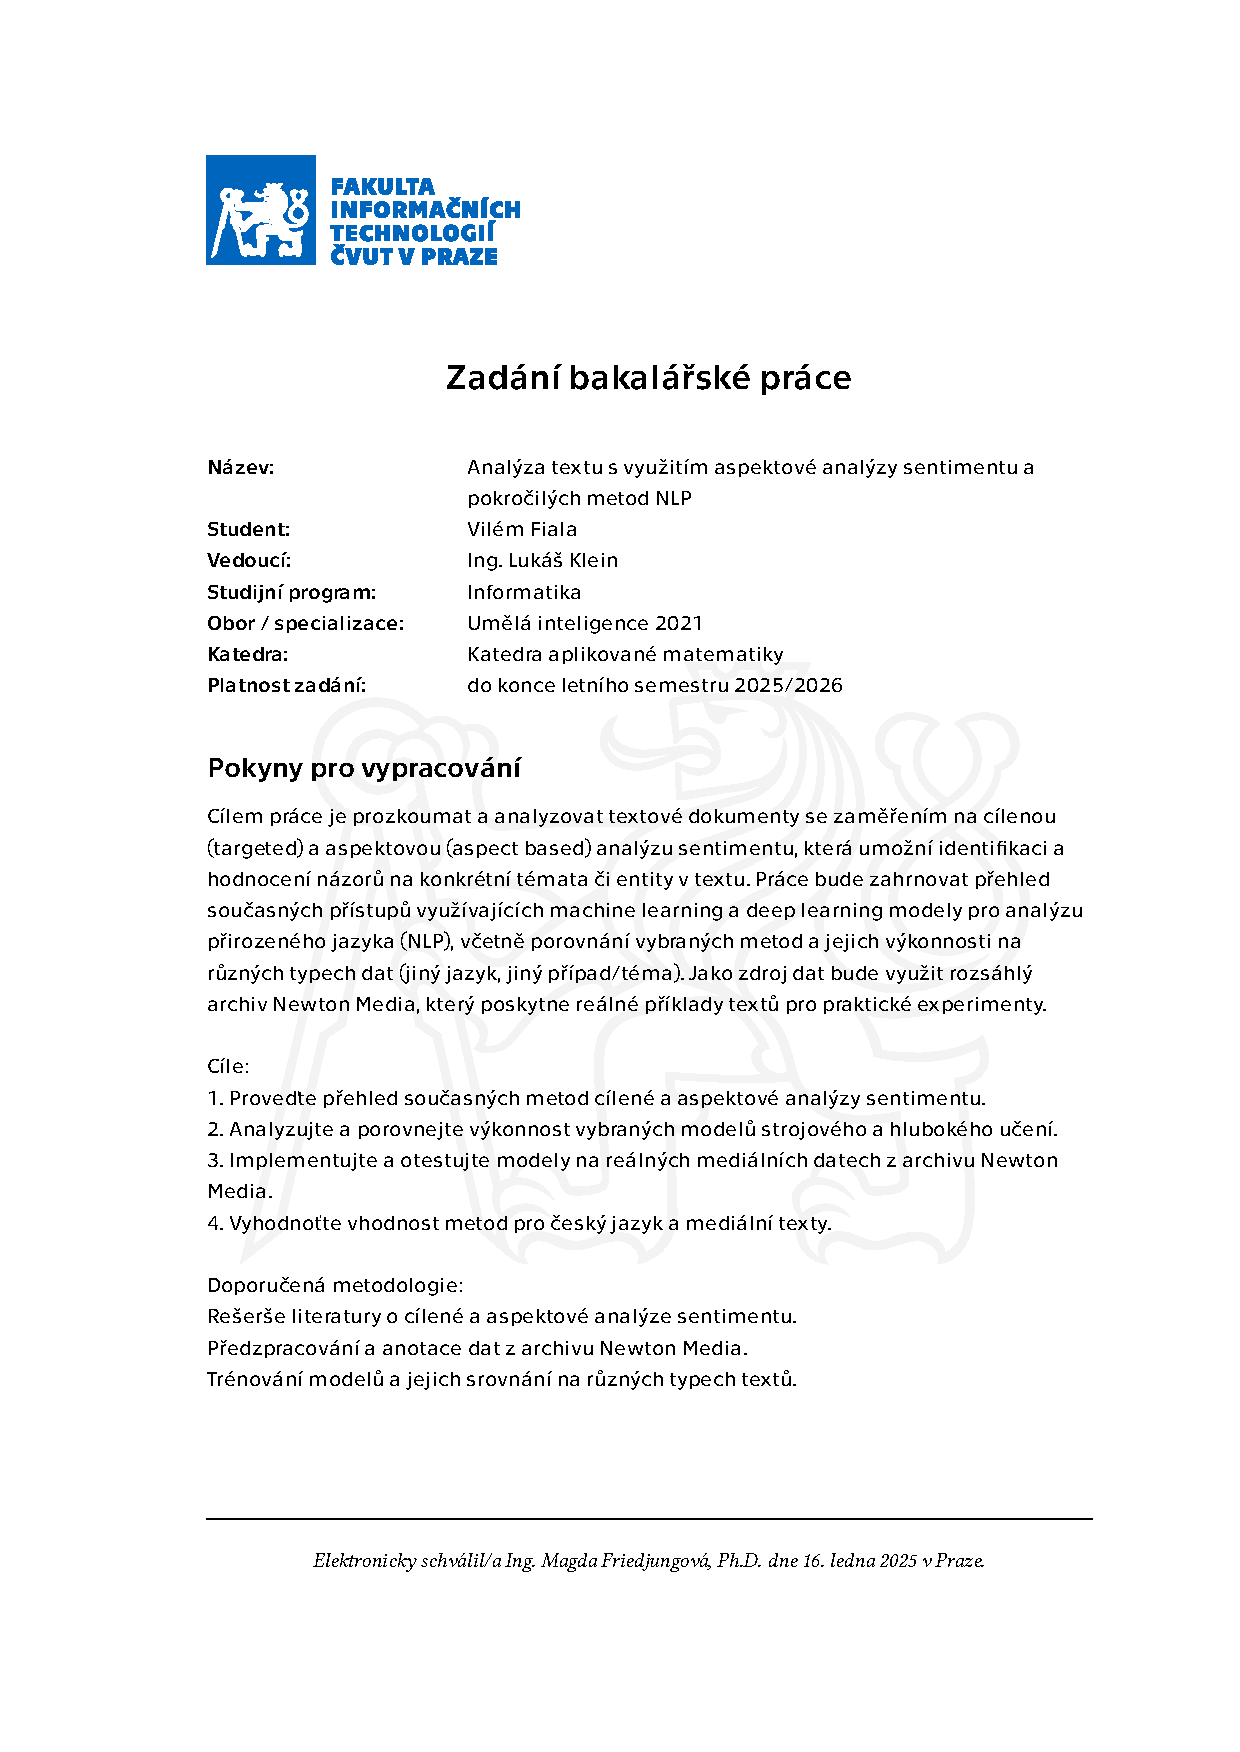
\includepdf[pages={1-}]{fialavi2-assignment.pdf} % replace this file with your thesis assignment generated from ProjectsFIT

\imprintpage % do not remove this command
\stopTOCentries
%%%%%%%%%%%%%%%%%%%%%%
% list of other contents END
%%%%%%%%%%%%%%%%%%%%%%

%%%%%%%%%%%%%%%%%%%
% ACKNOWLEDGMENT
% FILL IN / MODIFY
% This is a place to thank people for helping you. It is common to thank your supervisor.
%%%%%%%%%%%%%%%%%%%
\begin{acknowledgmentpage}
    Velmi rád bych poděkoval vedoucímu mé bakalářské práce, Ing. Lukáši Kleinovi, za cenné rady, podnětnou zpětnou vazbu a kontinuální podporu během celého procesu psaní. Mé poděkování rovněž patří společnosti Newton Media za poskytnutí prostoru k vypracování bakalářské práce v rámci mého pracovního zařazení. Dále děkuji Ing. Petře Pavlíčkové, Ph.D., za cenné konzultace a ochotu zodpovídat všechny mé dotazy, jež mi zásadně pomohly při samotném psaní.
\end{acknowledgmentpage} 
%%%%%%%%%%%%%%%%%%%
% ACKNOWLEDGMENT END
%%%%%%%%%%%%%%%%%%%


%%%%%%%%%%%%%%%%%%%
% DECLARATION
% FILL IN / MODIFY
%%%%%%%%%%%%%%%%%%%
% INSTRUCTIONS
% ENG: choose one of approved texts of the declaration. DO NOT CREATE YOUR OWN. Find the approved texts at https://courses.fit.cvut.cz/SFE/download/index.html#_documents (document Declaration for FT in English)
% CZE/SLO: Vyberte jedno z fakultou schvalenych prohlaseni. NEVKLADEJTE VLASTNI TEXT. Schvalena prohlaseni najdete zde: https://courses.fit.cvut.cz/SZZ/dokumenty/index.html#_dokumenty (prohlášení do ZP)
\begin{declarationpage}
Prohlašuji, že jsem předloženou práci vypracoval samostatně a že jsem uvedl veškeré použité informační zdroje v souladu s Metodickým pokynem o dodržování etických principů při přípravě vysokoškolských závěrečných prací.

Beru na vědomí, že se na moji práci vztahují práva a povinnosti vyplývající ze zákona č. 121/2000 Sb., autorského zákona, ve znění pozdějších předpisů. V souladu s ust. § 2373 odst. 2 zákona č. 89/2012 Sb., občanský zákoník, ve znění pozdějších předpisů, tímto uděluji nevýhradní oprávnění (licenci) k užití této mojí práce, a to včetně všech počítačových programů, jež jsou její součástí či přílohou a veškeré jejich dokumentace (dále souhrnně jen „Dílo“), a to všem osobám, které si přejí Dílo užít. Tyto osoby jsou oprávněny Dílo užít jakýmkoli způsobem, který nesnižuje hodnotu Díla a za jakýmkoli účelem (včetně užití k výdělečným účelům). Toto oprávnění je časově, teritoriálně i množstevně neomezené.

Prohlašuji, že jsem v průběhu příprav a psaní závěrečné práce použil nástroje umělé
inteligence. Vygenerovaný obsah jsem ověřil. Stvrzuji, že jsem si vědom, že za obsah
závěrečné práce plně zodpovídám.
\end{declarationpage}
%%%%%%%%%%%%%%%%%%%
% DECLARATION END
%%%%%%%%%%%%%%%%%%%

\printabstractpage % do not remove this command

%%%%%%%%%%%%%%%%%%%
% SUMMARY
% FILL IN / MODIFY
% OR REMOVE ENTIRELY (upon agreement with your supervisor)
% (appropriate to remove in most theses)
%%%%%%%%%%%%%%%%%%%
% \begin{summarypage}
% \section*{Summary section}
% 
% \lipsum[1][1-8]
% 
% \section*{Summary section}
% 
% \lipsum[2][1-6]
% 
% \section*{Summary section}
% 
% \lipsum[3]
% 
% \section*{Summary section}
% 
% \lipsum[2]
% 
% \section*{Summary section}
% 
% \lipsum[1][1-8] Lorem lorem lorem.
% \end{summarypage}
%%%%%%%%%%%%%%%%%%%
% SUMMARY END
%%%%%%%%%%%%%%%%%%%

\tableofcontents % do not remove this command
%%%%%%%%%%%%%%%%%%%%%%
% list of other contents: figures, tables, code listings, algorithms, etc.
% add/remove commands accordingly
%%%%%%%%%%%%%%%%%%%%%%
\listoffigures % list of figures
\listoftables % list of tables
\thectufitlistingscommand

%%%%%%%%%%%%%%%%%%%
% ABBREVIATIONS
% FILL IN / MODIFY
% OR REMOVE ENTIRELY
% List the abbreviations in lexicography order.
%%%%%%%%%%%%%%%%%%%
\chapter{\thectufitabbreviationlabel}
\begin{longtable}{rl}
ABSA & Aspect-based sentiment analysis \\
ACD & Aspect category detection \\
ACOS & Aspect-Category-Opinion-Sentiment Quadruple Extraction \\
ACSA & Aspect Category Sentiment Analysis \\
ALBERT & A Lite BERT \\
AOPE & Aspect-Opinion Pair Extraction \\
ASC & Aspect sentiment classification \\
ASTE & Aspect Sentiment Triplet Extraction \\
ATE & Aspect term extraction \\
BERT & Bidirectional Encoder Representations from Transformers \\
BPE & Byte-pair encoding \\
CLM & Conventional language models \\
CNN & Convolutional neural networks \\
DeBERTa & Decoding-enhanced BERT with Disentangled Attention \\
E2E-ABSA & End-to-End ABSA \\
FERNET & Flexible Embedding Representation NETwork \\
GPT & Generative Pre-training Transformer \\
LLM & Large language model \\
LM & Language model \\
LSTM & Long Short Term Memory \\
MAMS & Multi-Aspect Multi-Sentiment \\
mBERT & Multilingual BERT \\
MemN2N & End-to-End Memory Network \\
MemNN & Memory networks \\
NER & Named entity recognition \\
NB & Naive Bayes \\
NLG & Natural language generation \\
NLP & Natural language processing \\
NLU & Natural language understanding \\
OATS & Opinion Aspect Target Sentiment \\
OPE & Opinion term extraction \\
PLM & Pre-trained language models \\
RNN & Recurrent neural networks \\
RoBERTa & Robustly Optimized BERT Pretraining Approach \\
SRL & Semantic Role Labeling \\
SVM & Support vector machines \\
TASD & Target Aspect Sentiment Detection \\
UABSA & Unified ABSA \\
XLM & Cross-lingual language models \\
\end{longtable}
%%%%%%%%%%%%%%%%%%%
% ABBREVIATIONS END
%%%%%%%%%%%%%%%%%%%
\resumeTOCentries
\mainmatter\mainmatterinit % do not remove these two commands
%%%%%%%%%%%%%%%%%%%
% THE THESIS
% MODIFY ANYTHING BELOW THIS LINE
%%%%%%%%%%%%%%%%%%%

\chapter*{Úvod}\addcontentsline{toc}{chapter}{Úvod}\markboth{Úvod}{Úvod}


Analýza médií a textů je díky rychlému rozvoji umělé inteligence podstatně jednodušší než dříve. Firmy již nemusí zaměstnávat početné týmy pracovníků, kteří by osobně četli každý článek a na základě subjektivních pocitů jej hodnotili. Takové řešení navíc často přináší nekonzistentní výsledky, jelikož každý člověk může k hodnocení přistupovat odlišně. Proto se v současnosti stále více organizací obrací k umělé inteligenci, která -- po svém natrénování -- poskytuje konzistentní hodnocení.

Ne vždy je přitom nutné provádět detailní rozbor každého textu, mnohdy postačí obecná informace o celkovém sentimentu článku či recenze. Pro firmy nabízející široké portfolio produktů bývá důležité zejména to, jaký podíl recenzí je pozitivních a jaký negativních, což jim poskytuje rychlý přehled o vnímání jejich zboží ze strany zákazníků.

Problém však nastává, pokud jedna recenze či článek obsahuje kladné i záporné hodnocení. Například u notebooku si může autor recenze pochvalovat kvalitní obrazovku a dlouhou výdrž baterie, ale současně kritizovat nedostatečnou odolnost klávesnice. V takové situaci je vhodnější zaměřit se na konkrétní aspekty či témata a zjišťovat, jaký postoj k nim text zaujímá.

Cílený sentiment proto představuje užitečnou alternativu, kdy se text analyzuje s ohledem na zvolený aspekt a výsledkem je hodnocení vztahující se k tomuto aspektu. Tento postup umožňuje rychle identifikovat názor na vybrané aspekty a efektivně tak třídit či porovnávat texty podle konkrétních kritérií.

Zároveň však dnes neustále vznikají nové modely a metody, což klade nároky na uživatele, kteří musejí testovat různé přístupy a hledat nejvhodnější řešení pro svůj konkrétní problém. Analýza sentimentu v českém jazyce je navíc v porovnání s angličtinou stále poměrně málo rozšířená, což komplikuje výběr vhodného modelu a metod pro české texty a recenze.

\section*{Cíle}
\phantomsection
\addcontentsline{toc}{section}{Cíle}

Cílem této bakalářské práce je prozkoumat současné metody aspektové analýzy sentimentu v textu a otestovat vybrané postupy na různých typech dat v různých jazycích. Teoretická část bude zaměřena na vymezení problematiky zpracování přirozeného jazyka, analýzy sentimentu a popis vybraných metod i postupů. V praktické části budou vybrané metody aplikovány na data v češtině a v angličtině, vzájemně porovnány a vyhodnoceny z hlediska vhodnosti pro daný jazyk a konkrétní téma. Smyslem je najít či doporučit nejvhodnější metody pro práci s českými texty v kontextu mediálních textů.

\chapter{Zpracování jazyka pomocí umělé inteligence}\label{kapitola1}

Umělá inteligence pronikla do téměř všech oblastí lidské činnosti -- od generování a úprav multimediálního obsahu až po sofistikované predikční úlohy. Jednou z nejviditelnějších aplikací je v posledních letech zpracování textu, tedy schopnost strojově analyzovat a vytvářet přirozený jazyk. Významný rozvoj výpočetních kapacit a metod strojového učení umožnil vznik rozsáhlých modelů, které v řadě lingvistických úloh dosahují až lidské úrovně.

Tato kapitola nejprve představí základní principy zpracování přirozeného jazyka (NLP) a vymezí jeho roli v rámci širšího pole umělé inteligence. Následně se zaměří na jazykové modely jako klíčový nástroj praktického využití NLP. Popisuje jejich architektury i mechanismy učení, přičemž zvláštní pozornost je věnována modelům využitým v dalších částech této práce.

\section{Zpracování přirozeného jazyka -- NLP}\label{NLP}

\emph{Natural language processing} (NLP), v češtině zpracování přirozeného jazyka, spojuje poznatky z lingvistiky a umělé inteligence s cílem umožnit počítačům porozumět slovům a výrazům, jež lidé používají v běžném jazyce.~\cite{Khurana2023} Programovací jazyky (např.~C, C++ či Python) byly navrženy, aby programátoři mohli počítačům předávat přesné pokyny. Pro takovou komunikaci však musí člověk nejprve detailně zvládnout syntaxi a pravidla jazyka -- a i pak může drobná syntaktická či pravopisná chyba zabránit správnému provedení příkazu.

S přirozeným jazykem je to ale složitější. Když se v běžné komunikaci udělá menší chyba, často si druhá strana s pomocí kontextu domyslí, co bylo myšleno. Pro počítač je takové \uv{domýšlení} mnohem obtížnější. Právě to je jeden z úkolů, jimiž se NLP zabývá: vyvinout modely či algoritmy, které dokážou porozumět lidské řeči (byť s chybami) a provést zadané pokyny.

\subsection{Dvě základní složky NLP}
NLP se obvykle dělí na dvě hlavní části:
\begin{enumerate}
  \item \emph{Natural Language Understanding} (NLU) -- pochopení přirozeného jazyka.
  \item \emph{Natural Language Generation} (NLG)-- generování přirozeného jazyka.
\end{enumerate}

NLU umožňuje počítačům porozumět významu vět a slov, zachytit klíčové informace (např. emoce, zmíněné entity, hlavní témata) a rozpoznat, co je podstatou sdělení. NLG se naopak soustředí na tvorbu gramaticky a významově správných vět či textů.~\cite{Khurana2023} Tato práce se zaměřuje především na NLU, protože při analýze sentimentu -- tedy při zjišťování, jaký postoj daný text vyjadřuje -- se primárně texty zpracovávají a vyhodnocují,
aniž by musely být generovány.

\subsubsection{Pochopení přirozeného jazyka -- NLU}\label{NLU}

Jak již bylo zmíněno, cílem NLU je naučit počítač porozumět psanému textu v přirozeném jazyce. K tomu se využívají poznatky z lingvistiky, která se dále dělí na několik rovin; každá zachycuje odlišný aspekt jazyka a společně popisují informace v něm obsažené. Níže je uveden jejich stručný přehled převzatý z díla~\cite{Khurana2023}:

\paragraph{Fonologická rovina}
Zabývá se zvukovou stránkou jazyka. Zkoumá, jak jsou zvuky uspořádány a jak ovlivňují význam v komunikaci. V praxi se tak sleduje, jak se hlásky v jazyce kombinují a jak rozdílné zvukové podoby mohou měnit či vyjadřovat význam.

\paragraph{Morfologická rovina}
Zkoumá vnitřní strukturu slov a jejich nejmenší významové jednotky, tzv. morfémy. Každé slovo může být rozloženo na různé morfémy (např. předpony, kořen, přípony), které společně nesou určitý význam. Morfémy mají také různé funkce, např. předpony mohou být slovotvorné nebo tvarotvorné.~\cite{ujc-prirucka} Tímto způsobem lze pochopit a analyzovat význam, který se skrývá už v samotné struktuře slova.

\paragraph{Lexikální rovina}
Zaměřuje se na význam jednotlivých slov a jejich přiřazení k odpovídajícím slovním druhům (\emph{part-of-speech} tag). Pokud se jedno slovo může v různých kontextech chovat například jako podstatné jméno i sloveso, je na základě okolního textu určeno, který slovní druh v dané situaci plní. Součástí analýzy je také dělení textu na věty a slova, odstranění stop slov (např. \uv{a}, \uv{ale}, \uv{že}), a využití technik \emph{stemming} a \emph{lemmatizace}.
\begin{itemize}
  \item \textbf{Stemming} odstraňuje koncové části slov a redukuje je na jejich základní kořen. Například slova \uv{vařený} nebo \uv{vařit} by se mohla stáhnout ke tvaru \uv{vař}.
  \item \textbf{Lemmatizace} pracuje s jazykovými slovníky, aby identifikovala správný tvar slova včetně ohýbání či změn rodů a pádů (u slova \uv{vařil} či \uv{vařením} se hledá výchozí tvar \uv{vařit}).
\end{itemize}

\paragraph{Syntaktická rovina}
Zkoumá gramatickou strukturu vět a určuje vztahy mezi slovy. Po přiřazení slovních druhů na lexikální úrovni se slova seskupují do frází, které pak tvoří věty (\emph{parsing}). Tento postup sleduje správné pořadí slov a vazby mezi nimi. Na rozdíl od předchozí úrovně neodstraňuje stop slova ani neužívá lemmatizaci či stemming, protože by tím mohl pozměnit gramatický význam.

\paragraph{Sémantická rovina}
Soustředí se na odhalení skutečného významu věty a na rozlišení možných interpretací. Zohledňuje nejen slovní zásobu, ale také kontext a vztahy mezi slovy. Díky tomu lze poznat, že text pojednává například o filmu, i když výslovně neobsahuje slovo \uv{film} (stačí pojmy jako \uv{herec}, \uv{režisér} nebo \uv{scénář}). Součástí této úrovně je i řešení slov s více významy.

\paragraph{Diskurzní rovina}
Zabývá se významovými souvislostmi napříč vícero větami a zajišťuje tak celkovou návaznost textu. Zaměřuje se především na vztahy mezi výrazy, aby bylo zřejmé, že určitý zájmeno či jiný jazykový prvek odkazuje na předchozí jméno nebo entitu. Tato analýza je důležitá pro pokročilé úlohy, jako je automatická sumarizace či extrakce informací, protože pomáhá správně určit, kdo nebo co je v textu zmíněno.

\paragraph{Pragmatická rovina}
Zkoumá, jaký vliv na porozumění má kontext a reálné znalosti o světě, jež nejsou přímo obsaženy v textu. Soustředí se na to, co mluvčí skutečně zamýšlí říct a jak posluchač dané sdělení interpretuje na základě širších souvislostí. Díky pragmatické analýze lze rozlišit například, zda otázka \uv{Víte, kolik je hodin?} slouží k zjištění času, nebo spíše vyjadřuje nespokojenost se zpožděním. Tato rovina tak doplňuje čistě jazykové rozbory o význam, který se odvozuje i z mimojazykových faktorů.~\cite{Khurana2023}\\[0.3em]

Cílem zpracování přirozeného jazyka (NLP) je často sladit několik různých rovin tak, aby algoritmus či systém dokázal efektivně porozumět textu. Velkou výzvou přitom často bývá nejen kombinace více rovin, ale i řešení nejednoznačností, které se nejčastěji objevují v syntaktické, sémantické či lexikální rovině.~\cite{Khurana2023}

\subsection{Problematika vícejazyčného zpracování}\label{NLPjazyky}

Při zpracování přirozeného jazyka vychází každá lingvistická rovina z odlišných pravidel a charakteristik konkrétního jazyka. Rozdíly se týkají například abeced, směru psaní, výslovnosti, gramatiky, tvorby slov či struktury vět. Neexistuje proto jediné univerzální řešení, které by fungovalo stejně dobře pro všechny jazyky.

Tato práce se zaměřuje zejména na češtinu a angličtinu. Vzhledem k obrovskému rozšíření angličtiny -- podle statistik W3Techs přes 49\,\% webových stránek používá angličtinu jako základní jazyk (oproti 1\,\% v češtině)~\cite{w3techs-stats} -- je pro ni dostupné výrazně větší množství dat a zdrojů k trénování modelů. V českém prostředí je naopak často obtížnější získat dostatečně rozsáhlé a kvalitní datasety, což může omezovat přesnost metod vyvíjených pro češtinu.

\subsection{Využití NLP v praxi}

V předchozích částech byly popsány vlastnosti NLP a principy jeho jazykové analýzy. Metody NLP nacházejí široké uplatnění a dokážou zefektivnit celou řadu úkolů. Níže jsou uvedeny některé příklady, které tato práce dále podrobněji nerozebírá. Analýza sentimentu, na niž je tato práce soustředěna, bude předmětem kapitoly~\ref{sentiment}. Jednotlivé typy využití byly též zmíněny v díle~\cite{Khurana2023}:

\paragraph{Strojový překlad}
Umožňuje automatické převádění textů z jednoho jazyka do druhého. Kromě samotného překladu slov se klade důraz na zachování významu, gramatických vazeb i kontextu, aby byl výsledný text srozumitelný a co nejbližší originálu.

\paragraph{Kategorizace textu}
Slouží k automatickému třídění rozsáhlých množství dokumentů (např. zprávy, oficiální spisy, tržní data) do předem definovaných kategorií. Urychluje vyhledávání a usnadňuje následné zpracování velkých datových souborů.

\paragraph{Extrakce informací}
Cílem je rozpoznat a vytáhnout důležité prvky z textu, například jména osob, místa či události. Tato informace se dále využívá pro sumarizaci, budování databází nebo jako vstup pro další analýzy.

\paragraph{Sumarizace}
Z textu se automaticky vytváří kratší přehled, který vystihuje klíčové informace. Umožňuje rychlé seznámení s obsahem rozsáhlých dokumentů či vícero zdrojů najednou.

\paragraph{Dialogové systémy}
Zahrnují chatovací asistenty nebo hlasové pomocníky. Na základě jazykové analýzy rozumějí dotazům uživatele a generují odpovědi nebo vykonávají zadané úkoly (například vyhledání informací či nastavení budíku).~\cite{Khurana2023}

\section{Jazykové modely -- LM}\label{LM}
V předchozí sekci~\ref{NLP} bylo naznačeno, jakým způsobem může být poskytnuta možnost pro běžného uživatele komunikovat se systémem v přirozeném jazyce, a jak se počítač pokouší porozumět zadaným pokynům. Nastává však otázka, jakým způsobem takovou komunikaci reálně implementovat a jak naprogramovat modely, které dokážou zpracovávat a analyzovat text prostřednictvím NLP. Tato problematika je řešena pomocí LM (\emph{Language models}, česky jazykové modely).

Pojem \emph{jazykové modely} je velmi obecný a zahrnuje řadu přístupů s různou hloubkou i rozsahem. Starší definice často zmiňují nástroj, který na základě rozsáhlé databáze textů přiřazuje větám či slovům určitou pravděpodobnost. Jde tedy o systém, jenž vychází z trénovacího korpusu a následně posuzuje, jak „pravděpodobná“ je daná sekvence slov. Lze si jej představit jako komplexní vyhledávací databázi, která na základě podobností generuje možné textové výstupy.~\cite{Hiemstra2009}

Moderní přístupy staví zejména na neuronových sítích. Ty se po zpracování velkého množství dat naučí strukturu a generování textu efektivněji než tradiční statistické metody.~\cite{Wei_2024} Přesto zůstává základní myšlenka stejná: cílem je naučit se pravděpodobnostní rozdělení jazykových jednotek (například slov a vět), a to tak, aby model dokázal předvídat či tvořit text na základě naučeného kontextu.

Tyto dvě definice společně ukazují dva hlavní přístupy, jak k tvorbě jazykových modelů lze přistupovat:~\cite{Wei_2024, zhou2023comprehensivesurveypretrainedfoundation}

\begin{itemize}
    \item \textbf{Statistický (klasický) přístup} -- založený na myšlence, že pravděpodobnost určitého slova závisí na jeho předchozím kontextu. Cílem je sestavit pravděpodobnostní rozdělení nad posloupnostmi slov pomocí četností v trénovacím korpusu. Mezi známé statistické přístupy patří např. N-gram modely~\cite{brown-etal-1992-class}.
    \item \textbf{Neuronový (data-driven) přístup} -- vychází z trénování neuronové sítě. Model se učí přímo z velkých objemů neupravených dat, čímž si buduje bohatou představu o slovech, frázích i kontextu. Mezi známe patří GPT~\cite{radford2018improving} a BERT~\cite{devlin2019bert}.
\end{itemize}

Toto rozdělení nás přivádí k rozlišení CLMs (\emph{Conventional Language Models}, česky konvenční či klasické jazykové modely) a PLMs (\emph{Pre-trained Language Models}, česky předtrénované jazykové modely)~\cite{Wei_2024}. Tato práce se zaměří na PLMs, jelikož klasické statistické metody (CLMs) se dnes téměř nepoužívají a zároveň je velmi snadné PLMs implementovat či dotrénovat pomocí dostupných nástrojů, například prostřednictvím webového portálu Hugging Face~\cite{huggingface}.

Než budou představeny PLMs, je nejprve nutné text vhodně předzpracovat. Počítače totiž dokážou efektivněji ukládat slova, než aby si pamatovaly každý jednotlivý znak. K tomuto účelu slouží tokenizace.

\subsection{Tokenizace}
Než model začne zpracovávat text a učit se jeho strukturu, je třeba rozhodnout, v jaké formě bude tento text zpracovávat. Měl by text chápat jako lidé, tedy rozdělovat ho na slova, nebo i na víceslovné výrazy? A nebo jej rozdělit kompletně na jednotlivá písmena? To jsou otázky, kterými se vědci a programátoři zabývají již dlouho (viz studie z roku 1992~\cite{webster-kit-1992-tokenization}).

Donedávna většina modelů pro NLP používala slova jako hlavní jednotku textu, ale s příchodem byte-pair encoding (BPE) se přešlo na části slov, tedy na \emph{tokeny}. Díky tokenům se daly zmenšit slovníky modelů, aniž by došlo ke ztrátě důležitých informací. Tokeny mají více definic, ale obecně lze říci, že se jedná o tzv. \emph{typografickou jednotku}, která je pro model nejlogičtější pro zpracování~\cite{mielke2021wordscharactersbriefhistory}.

\subsubsection{Tokeny v různých jazycích}\label{TokenJaz}
Jak již bylo naznačeno v podsekci~\ref{NLPjazyky}, každý jazyk má odlišnou gramatiku a pravidla, což se odráží i na způsobu tokenizace. Některé jazyky je možné snadněji převést na tokeny, zatímco u jiných bude potřeba více tokenů pro zachování významu jednoho slova.

Například záleží, zda jazyk obsahuje pády, či nikoli. V jazycích s pády, jako je čeština, jedno slovo může být reprezentováno více tokeny v závislosti na kontextu. Jednoduchým příkladem je slovo \uv{ty} v češtině a \uv{you} v angličtině. V angličtině zůstává \uv{you} vždy stejné, zatímco v češtině bude záviset na pádu -- může to být například ve 2. pádu \uv{tebe}, ve 3. pádu \uv{tobě} a tak dále. Tento faktor způsobuje, že slovník tokenů pro češtinu bude mnohem větší než pro angličtinu.

V článku~\cite{tokenizacemultilingual} autorka zkoumá, jak funguje tokenizace v různých jazycích. Jako příklad je uvedena věta: \uv{Jaké bude počasí příští týden}, která byla analyzována v pěti různých jazycích. V angličtině a španělštině měla tato věta 7, respektive 8 tokenů, zatímco v barmštině (jazyk v Myanmaru) a amharštině (jazyk v Etiopii) měla 61, respektive 69 tokenů, což je téměř desetkrát více. Podrobnější popis této problematiky je uveden v již zmíněném článku~\cite{tokenizacemultilingual}.

\subsection{Předtrénované jazykové modely -- PLMs}\label{PLMs}
Předtrénované jazykové modely patří v současné době mezi nejvyužívanější nástroje v oblasti NLP. Jedná se o rozsáhlé neuronové sítě založené na transformátorové architektuře, které lze nasadit na širokou škálu úloh. Velká část jejich schopností vychází z faktu, že jsou nejprve natrénovány na rozsáhlých a různorodých korpusech, kde si osvojují znalost syntaxe, sémantiky a dalších jazykových jevů (viz též \ref{NLU}). Poté lze modely jemně doladit (tzv. \emph{fine-tuning}) pro specifické použití.~\cite{Wei_2024, zhou2023comprehensivesurveypretrainedfoundation, min2021recentadvancesnaturallanguage, Elazar2021}

V této práci bude takový typ modelů využit pro úlohu rozpoznávání sentimentu. Díky již nabyté znalosti struktury textu v češtině i angličtině postačí model následně specializovaně dotrénovat tak, aby přesně klasifikoval náladu či postoj vyjádřený v daném textu, a to na základě vybraného trénovacího datasetu.

V následujících podsekcích jsou popsány stěžejní vlastnosti předtrénovaných jazykových modelů (PLM). Nejprve je představena jejich architektura, poté je přiblížen postup samotného předtrénování a nakonec je ukázáno, jak lze tyto modely doladit (\emph{fine-tuning}) pro konkrétní úlohy.

\subsubsection{Transformátorová architektura}\label{Transformator}
Transformátor~\cite{vaswani2023attentionneed} představuje vylepšenou architekturu oproti rekurentním a konvolučním neuronovým sítím a postupně je nahradil v mnoha úlohách. Místo rekurence pracuje pouze s \emph{mechanismem pozornosti} (attention mechanism), který dokáže zachytit globální závislosti mezi vstupem a výstupem. Díky tomu je velmi flexibilní (tzv. vysoce parametrizovatelná) a umožňuje vznik pokročilých modelů, jako jsou například GPT~\cite{radford2018improving} nebo BERT~\cite{devlin2019bert}.

Funkci pozornosti lze popsat jako mapování dotazu a sady klíč--hodnota na výstup, který je váženým součtem hodnot, váhy se odvozují z porovnání dotazu s příslušným klíčem. Namísto jedné takovéto pozornosti používá transformátor tzv. \emph{multi-head attention}, jež poskytuje bohatší pohled na reprezentaci dat. Detailní popis \emph{multi-head attention} i celé transformátorové architektury lze nalézt v původní práci~\cite{vaswani2023attentionneed}.

\subsubsection{Předtrénování}\label{predtrenovani}
Předtrénování je klíčovou součástí moderní přípravy modelů. Dnes už není nutné trénovat každý model od začátku; místo toho stačí využít předtrénovaný model, který si lze stáhnout z dostupných portálů (například již zmíněného Hugging Face~\cite{huggingface}), a následně ho dotrénovat na specifický úkol pomocí menšího datasetu. Díky tomu, že byly modely natrénovány na rozsáhlých a různorodých datech, dokážou zachytit nuance v různých jazycích a efektivně reagovat na úkoly.

Existuje mnoho metod předtrénování, které závisí na konkrétní úloze, pro kterou je model připravován. Nejznámější a nejčastěji používanou metodou je \emph{missing token prediction} (predikce chybějícího tokenu). Kromě této metody existuje i řada dalších přístupů, jako např. \emph{next-sentence prediction} (predikce následující věty) nebo \emph{replaced token prediction} (predikce vyměněného tokenu).~\cite{Wei_2024, zhou2023comprehensivesurveypretrainedfoundation}

\paragraph{Missing token prediction}
Tento typ trénování využívají jak autoregresní jazykové modely (např. GPT~\cite{radford2018improving}), tak i maskované jazykové modely (např. BERT~\cite{devlin2019bert}). Cílem je pomocí určitých tokenů (slov) predikovat okolní nebo následující tokeny. Maskované jazykové modely jsou trénovány tak, že se přibližně 15\% tokenů zamaskuje a pomocí zbytku se model snaží tyto maskované tokeny predikovat. U autoregresivních jazykových modelů se na základě dané sekvence tokenů predikuje následující token v řadě. Hlavní rozdíl spočívá v tom, že první typ modelu predikuje tokeny v závislosti na všech dostupných, což zlepšuje celkový přehled o struktuře textu. Druhý přístup je vhodnější pro generaci slov, protože na základě určitých tokenů dokáže model vygenerovat zbytek textu.~\cite{Wei_2024, min2021recentadvancesnaturallanguage}

\paragraph{Další metody předtrénování}
Jak již bylo zmíněno, existuje řada dalších metod předtrénování. \emph{Next-sentence prediction} vybírá dvě věty a predikuje, zda druhá věta skutečně následuje po té první, čímž ověřuje správnost jejich pořadí. \emph{Replaced token prediction} se zaměřuje na kontrolu, zda byly některé tokeny v textu vyměněny. Podrobnější popis těchto metod a dalších je k nalezení v těchto studiích~\cite{Wei_2024, zhou2023comprehensivesurveypretrainedfoundation}.

\subsubsection{Fine-tuning}
V předchozí podsekci~\ref{predtrenovani} bylo popsáno, proč je předtrénování klíčové a jak model získává základní znalost jazyka. Fine-tuning (dotrénování) tento již existující model přizpůsobuje konkrétnímu úkolu, například klasifikaci sentimentu nebo rozpoznávání pojmenovaných entit.  

Nejběžnější přístup spočívá v tom, že se celý model znovu trénuje (resp. aktualizují se všechny jeho vrstvy) na menším datasetu určeném pro danou úlohu. Nevýhodou takového postupu ale je, že i při malé změně úkolu je nutné trénovat model od začátku, což je výpočetně náročné.~\cite{Wei_2024, min2021recentadvancesnaturallanguage}

Proto se často používá tzv. \emph{Adapter tuning}~\cite{pfeiffer-etal-2021-adapterfusion, houlsby2019parameterefficienttransferlearningnlp}, při němž se do modelu přidají speciální vrstvy (adapters) s relativně malým počtem parametrů. Během trénování se upravují pouze tyto adaptéry, zatímco původní parametry modelu zůstávají beze změny. Díky tomu lze jeden předtrénovaný model efektivně použít pro více odlišných úkolů, neboť stačí vyměnit jen konkrétní adaptéry místo kompletního přeučování celého modelu.~\cite{Wei_2024, min2021recentadvancesnaturallanguage} Pro rozsáhlé modely jako GPT-3, který má 175 miliard parametrů~\cite{brown2020languagemodelsfewshotlearners}, je tento přístup časově i výpočetně výrazně úspornější.

\subsection{Decoder vs Encoder}\label{DECENC}

V podsekci~\ref{predtrenovani} byly představeny dva rozdílné přístupy k trénování jazykových modelů. Modely trénované prvním přístupem jsou označovány jako \emph{autoregresivní jazykové modely}, zatímco druhým jako \emph{maskované jazykové modely}. Toto rozdělení vede k modelům \emph{Decoder-only} a \emph{Encoder-only}, které se liší nejen v přístupu k trénování, ale i v architektuře transformátoru. Architektura transformátoru obsahuje strukturu \emph{encoder-decoder}, kterou lze rozdělit na dvě samostatné komponenty~\cite{vaswani2023attentionneed}. Tato možnost vedla k vytvoření modelů jako je GPT~\cite{radford2018improving}, které využívají pouze decoder, a BERT~\cite{devlin2019bert}, který využívá pouze encoder.

\subsubsection{Decoder-only modely}
Díky velkému nárůstu zájmu o LLMs~\cite{minaee2025largelanguagemodelssurvey, naveed2024comprehensiveoverviewlargelanguage} (\emph{Large language models}, česky velké jazykové modely) se v současnosti věnuje většina pozornosti decoder-only neboli \emph{generativním modelům}. Ty dokážou generovat texty působící jako lidské a zvládají interaktivní konverzaci. Na encoder-only modely se přitom často zapomíná.~\cite{modernbertreplacment}

Současné generativní modely jsou však obvykle velmi rozsáhlé, pomalé a nákladné pro většinu úkolů. Přestože zvládnou všechno, co encoder-only modely a ještě více, existují situace, kdy je potřeba zpracovávat úlohy rychle a ve velkém množství. V takových případech je vhodnější menší model s nižšími nároky na výpočetní zdroje. Proto mají encoder-only modely stále své místo a praktické využití.~\cite{modernbertreplacment}

\subsubsection{Encoder-only modely}

Výstup encoder-only modelů není text (jako u decoder-only modelů), nýbrž seznam hodnot (tzv. \emph{embedding vector}). Místo generování slov tedy model svou odpověď \uv{zakóduje} do vektorové reprezentace, jež lze následně interpretovat nebo použít v jiné nadstavbové úloze. Proto se encoder-only modely někdy označují jako \emph{reprezentační modely}~\cite{modernbertreplacment}.

Jak již bylo zmíněno, decoder-only modely mohou v principu plnit stejnou funkci jako encoder-only modely, avšak při čistě analytických úkolech může být jejich autoregresivní charakter nevýhodou. Encoder-only modely, díky jejich architektuře, jsou vhodnější pro rychlé a rozsáhlé analýzy textu, ať už jde o klasifikaci, detekci entit nebo jiné úlohy. Další přednosti encoder-only modelů jsou podrobně rozebrány například v blogu o modelu ModernBERT~\cite{modernbertreplacment}.

\subsubsection{Jaký model pro sentiment?}
Jelikož je v této práci hlavním cílem analyzovat sentiment textu, není nutná jeho generace. Stačí tedy číselná reprezentace, která vyjádří, jaký sentiment daný text má. Z tohoto důvodu jsou v této práci využity \emph{encoder-only} modely, konkrétně BERT~\cite{devlin2019bert} a jeho následné varianty, jako např. RoBERTa~\cite{liu2019robertarobustlyoptimizedbert} či ModernBERT~\cite{warner2024smarterbetterfasterlonger}.

\chapter{Analýza sentimentu}\label{sentiment}

V předchozí kapitole~\ref{kapitola1} bylo ukázáno, jak počítače zpracovávají lidský jazyk, a také byly představeny moderní jazykové modely založené na transformátorové architektuře. Tato kapitola bude zamířena na jedno z důležitých využití NLP a jazykových modelů -- \emph{analýzu sentimentu}, jež představuje hlavní téma této práce.

S rozvojem internetu získali lidé z nejrůznějších prostředí prostor pro veřejné komentáře a sdílení názorů -- ať už jde o recenze produktů, diskuze o politice nebo komentáře ke známým osobnostem. Každý den tak vzniká obrovské množství textových dat, která sama o sobě nenabízejí přímou hodnotu. Již kolem roku 2003 proto začaly vznikat první výzkumy~\cite{NasukawaSA}, jejichž cílem bylo najít způsoby, jak tuto textovou \uv{zpětnou vazbu} analyzovat a využívat v praxi. Firmy tak mohou pomocí analýzy sentimentu odhalit postoje svých zákazníků, lépe řídit vývoj nových produktů a cíleněji směřovat své služby.~\cite{Aqlanstudyofsentiment}

Analýza sentimentu, někdy nazývaná také \emph{opinion mining}, slouží k zjišťování názorů, pocitů a reakcí uživatelů na internetu, zejména na sociálních sítích či obchodních portálech. Typicky se využívá ke klasifikaci textů (např. recenzí či komentářů) do kategorií \uv{pozitivní}, \uv{negativní} a \uv{neutrální}. S rozmachem sociálních sítí se oblasti, které chtějí pochopit názory uživatelů -- jako politici, výrobci, vědci či psychologové --, zaměřují právě na tuto formu textové analýzy. Analýza sentimentu stojí na kombinaci metod zpracování přirozeného jazyka (NLP), statistiky a strojového učení, a snaží se tak efektivně zachytit a definovat \uv{náladu} či postoj v textu.~\cite{Aqlanstudyofsentiment}

Analýza sentimentu se nemusí omezovat pouze na psaný text, protože emoce a postoje lze rozpoznávat i z dalších druhů obsahu. Například v řečovém projevu se vyhodnocuje tón hlasu, rytmus, intonace a způsoby vyjadřování, z nichž lze usuzovat zaujetí či emocionalitu mluvčího. U fotografií nebo videí se pak zkoumají neverbální signály, jako jsou mimika, gesta a celková kompozice, které mohou vypovídat o náladě či názoru zobrazovaných osob. Dalším příkladem jsou tzv. memy, podle kterých se dá sledovat nálada uživatele, který tento meme zveřejnil. Pokud se propojí více druhů médií (audio, video a text), hovoříme o tzv. \emph{multimodální analýze sentimentu}.~\cite{kumar2023comprehensivereviewsentimentanalysis} V této práci se však pozornost soustředí výhradně na analýzu sentimentu v textu.

\section{Techniky analýzy sentimentu}\label{TechAnaSen}
K analýze sentimentu lze přistupovat různými způsoby, které se liší technickým zázemím i mírou využití jazykových modelů, představených v sekci~\ref{LM}. Zpravidla se rozlišují metody slovníkové (lexicon-based), tradiční přístupy strojového učení, hluboké učení (neuronové sítě) a hybridní řešení. K modernějším technikám pak patří postupy založené na transformátorové architektuře (viz podsekce~\ref{Transformator}). Podrobný přehled výhod a nevýhod těchto metod i jejich konkrétních možností nasazení lze nalézt v díle~\cite{MAO2024102048}.

V této práci je pro analýzu sentimentu zvolen přístup využívající transformátorové modely, jak bylo podrobněji popsáno v sekci~\ref{PLMs}. Díky mechanismu pozornosti (attention) tyto modely lépe zachycují kontext a jemné jazykové nuance, a proto mnohdy překonávají klasické techniky analýzy sentimentu v přesnosti i rozsahu využití.

\subsection{Slovníková metoda}
Slovníkový přístup vychází z předpokladu, že některá slova bývají tradičně vnímána jako \uv{pozitivní} a jiná jako \uv{negativní}. Tato slova se shromažďují v tzv. slovnících (lexikonech), podle nichž se následně určuje sentiment textu. Rozlišují se přitom dva základní postupy, korpusový a slovníkový, přičemž každý z nich má své specifické výhody i nevýhody. Detailnější přehled této metody lze nalézt v pracích~\cite{Aqlanstudyofsentiment, MAO2024102048}.

\subsection{Tradiční přístupy strojového učení}
Tradiční metody strojového učení vycházejí z rozdělení dat na trénovací a testovací sadu. Model se na trénovací sadě naučí rozlišovat sentiment (případně jiné charakteristiky) a poté se ověří na dosud neviděných datech z testovací sady. Příkladem takových postupů jsou Naivní Bayes (NB), Metoda podpůrných vektorů (SVM) nebo rozhodovací stromy~\cite{MAO2024102048}. Různé studie zkoumající nasazení těchto tradičních metod v analýze sentimentu jsou přehledně popsány v~\cite{SuryawanshiSA}.

\subsection{Hluboké učení}
Kvůli nedostatečnému výpočetnímu výkonu nebylo možné hluboké učení (neuronové sítě) důkladně zkoumat. Avšak díky výraznému technologickému pokroku, zejména v oblasti grafických procesorů (GPU), získaly neuronové sítě na výkonnosti a možnosti využití. Hluboké učení využívá kaskádu více vrstev nelineárních zpracovatelských jednotek pro extrakci a transformaci příznaků. Nižší vrstvy, které jsou blízko vstupním datům, se učí jednoduché rysy, zatímco vyšší vrstvy zachycují složitější vlastnosti, jež jsou odvozeny z příznaků získaných v nižších vrstvách.~\cite{zhang2018deeplearningsentimentanalysis}

V této sekci budou představeny nejpoužívanější typy neuronových sítí v oblasti NLP, a to zejména konvoluční neuronové sítě (\emph{Convolutional Neural Networks, CNN}), rekurentní neuronové sítě (\emph{Recurrent Neural Networks, RNN}) a sítě s dlouhou krátkodobou pamětí (\emph{Long Short Term Memory networks, LSTM}). Jednotlivé typy neuronových sítí jsou zde popsány pouze stručně, zatímco podrobnější informace lze nalézt v díle~\cite{zhang2018deeplearningsentimentanalysis}. Přehled studií zkoumajících využití těchto metod v praxi je uveden v~\cite{SuryawanshiSA}.

\subsubsection{Konvoluční neuronové sítě}
Konvoluční neuronová síť (CNN) je druh dopředné neuronové sítě, který byl původně vyvíjen pro úlohy spojené s počítačovým viděním. Její architektura čerpá inspiraci z lidské zrakové kůry (vizuální mechanismus přítomný v mozku živočichů). Tato zraková kůra obsahuje početné skupiny buněk citlivých na světlo v malých, vzájemně se překrývajících oblastech zorného pole, jež se označují jako receptivní pole. Tyto buňky fungují jako lokální filtry, které přenášejí informace o vstupních signálech dále. CNN se proto skládá z několika konvolučních vrstev, přičemž každá vrstva napodobuje funkci zmíněných buněk v zrakovém centru.~\cite{zhang2018deeplearningsentimentanalysis}

\subsubsection{Rekurentní neuronové sítě}
Rekurentní neuronová síť (RNN)~\cite{RNNbib} je typ neuronové sítě, ve které jsou spojení mezi neurony uspořádána do směrovaného cyklu. Na rozdíl od dopředných neuronových sítí dokáže díky své vnitřní  \uv{paměti} zpracovávat i sekvenční data. Tato  \uv{paměť} znamená, že pro každý prvek vstupní sekvence používá RNN stejné operace, přičemž výstup v každém kroku závisí na všech dosavadních výpočtech. Tímto způsobem si RNN  \uv{pamatuje} kontext již zpracovaných prvků a uplatňuje jej při dalším výpočtu.~\cite{zhang2018deeplearningsentimentanalysis}

\subsubsection{Sítě s dlouhou krátkodobou pamětí}
Síť s dlouhou krátkodobou pamětí (LSTM)~\cite{LSTMbib} představuje speciální druh RNN schopný pracovat s dlouhodobými závislostmi. Všechny RNN lze popsat jako řetězec opakujících se modulů, avšak u klasické RNN je tento modul zpravidla jednoduchý, zatímco LSTM využívá složitější vnitřní strukturu. Namísto jedné vrstvy neuronů obsahuje čtyři, které spolu vzájemně specifickým způsobem komunikují.~\cite{zhang2018deeplearningsentimentanalysis}

\subsubsection{Další metody hlubokého učení v NLP}
Neuronové sítě a hluboké učení nejsou omezeny pouze na výše popsané tři typy. Existuje řada dalších přístupů a využití, která zde budou zmíněna jen stručně, podrobnější informace lze nalézt v díle~\cite{zhang2018deeplearningsentimentanalysis}.

\paragraph{Mechanismus pozornosti s RNN}
Aby bylo možné lépe zachytit dlouhodobé závislosti, s nimiž měly RNN a LSTM obtíže, začal se využívat mechanismus pozornosti, inspirovaný vizuální pozorností u člověka. Prvně byl aplikován u strojového překladu v NLP~\cite{bahdanau2016neuralmachinetranslationjointly}. Tyto sítě využívaly strukturu \emph{encoder-decoder}, která byla již letmo představena v sekci~\ref{DECENC} a později se stala hlavním stavebním kamenem transformátorové architektury.~\cite{zhang2018deeplearningsentimentanalysis}

\paragraph{Paměťové sítě}
Paměťové sítě (\emph{Memory networks, MemNN}) byly původně představeny v souvislosti s úlohou odpovídání na otázky~\cite{weston2015memorynetworks}. Využívají několik inferenčních komponent v kombinaci s velkou dlouhodobou pamětí, přičemž tyto komponenty mohou být tvořeny neuronovými sítěmi. Na jejich základě vznikla vylepšená verze End-to-End paměťová síť (\emph{End-to-End Memory network, MemN2N})~\cite{sukhbaatar2015endtoendmemorynetworks}, která kombinuje mechanismus pozornosti a práci s dlouhodobou pamětí.~\cite{zhang2018deeplearningsentimentanalysis}

\paragraph{Rekurzivní neuronové sítě}
Rekurzivní neuronové sítě (\emph{Recursive neural networks, RecNN}) představují typ neuronových sítí, které se obvykle používají k práci s řízenými acyklickými grafy (typicky stromovými strukturami). Jedná se o obecnější variantu rekurentních neuronových sítí (RNN).~\cite{zhang2018deeplearningsentimentanalysis}


\subsection{Hybridní metoda}
Jak název napovídá, hybridní metoda propojuje více přístupů -- například kombinuje charakteristiky slovníkových metod a strojového učení, aby využila silné stránky jednotlivých modelů a kompenzovala jejich slabiny~\cite{Aqlanstudyofsentiment}.

\section{Úrovně analýzy sentimentu}

Výzkumníci obvykle zkoumají sentiment na třech základních úrovních podrobnosti: \emph{dokumentové}, \emph{větné} a \emph{aspektové}.~\cite{MAO2024102048, zhang2018deeplearningsentimentanalysis}

\subsection{Dokumentová úroveň}
Klasifikace na dokumentové úrovni posuzuje celý text (např. recenzi produktu) jako jeden celek a určuje, jaký vyjadřuje postoj. Dokument se typicky zaměřuje na jednu entitu (např. \uv{telefon}) a snaží se posoudit její celkový sentiment.~\cite{zhang2018deeplearningsentimentanalysis}

Z pohledu analýzy sentimentu se v rámci této úrovně často pracuje jako s klasifikací dokumentu do tří tříd (pozitivní, negativní a neutrální). Tradičně se využíval přístup \emph{Bag of Words}, který s textem zachází jako s množinou slov bez ohledu na pořadí. O výsledném sentimentu rozhodovala frekvence nebo přítomnost určitých výrazů. Později se začaly prosazovat neuronové sítě, které využívají kódování slov do tzv. \emph{dense vectors}, které dokáží zakódovat informace o sémantických a syntaktických vlastnostech. Podrobnější informace o těchto přístupech a přehled výzkumů zaměřených na dokumentovou úroveň sentimentu lze nalézt v~\cite{zhang2018deeplearningsentimentanalysis}.

\subsection{Větná úroveň}
Na této úrovni se sentiment klasifikuje pro jednotlivé věty v textu. Obvykle se nejprve rozhoduje, zda věta vůbec vyjadřuje názor či nikoliv (tzv. \emph{subjectivity classification}), a teprve následně se stanovuje, jestli je vyjádřený sentiment pozitivní, negativní, nebo neutrální (tzv. \emph{polarity classification})~\cite{zhang2018deeplearningsentimentanalysis}.

Samotná predikce sentimentu pak probíhá podobně jako u dokumentové úrovně, ale vzhledem ke kratšímu rozsahu vět lze efektivněji využít i detailnější syntaktické a sémantické informace. Podrobnější informace o analýze sentimentu na větné úrovni a přehled souvisejících výzkumů jsou uvedeny v~\cite{zhang2018deeplearningsentimentanalysis}.

\subsection{Aspektová úroveň}
Aspektová úroveň představuje nejdetailnější formu analýzy sentimentu, protože nezkoumá pouze celkový sentiment textu, ale soustředí se na jednotlivé vlastnosti (\emph{aspekty} nebo \emph{cíle}) konkrétní entity.~\cite{zhang2018deeplearningsentimentanalysis} Tato úroveň představuje hlavní zaměření této práce, neboť umožňuje nejpřesněji interpretovat recenze či analyzovat mediální texty, například s cílem zjistit, jak jsou v novinových článcích hodnoceny různé firmy nebo osobnosti. Podrobnější popis celé problematiky aspektové analýzy sentimentu bude v následující sekci~\ref{absa}.

\begin{figure}[!htbp]
    \centering
    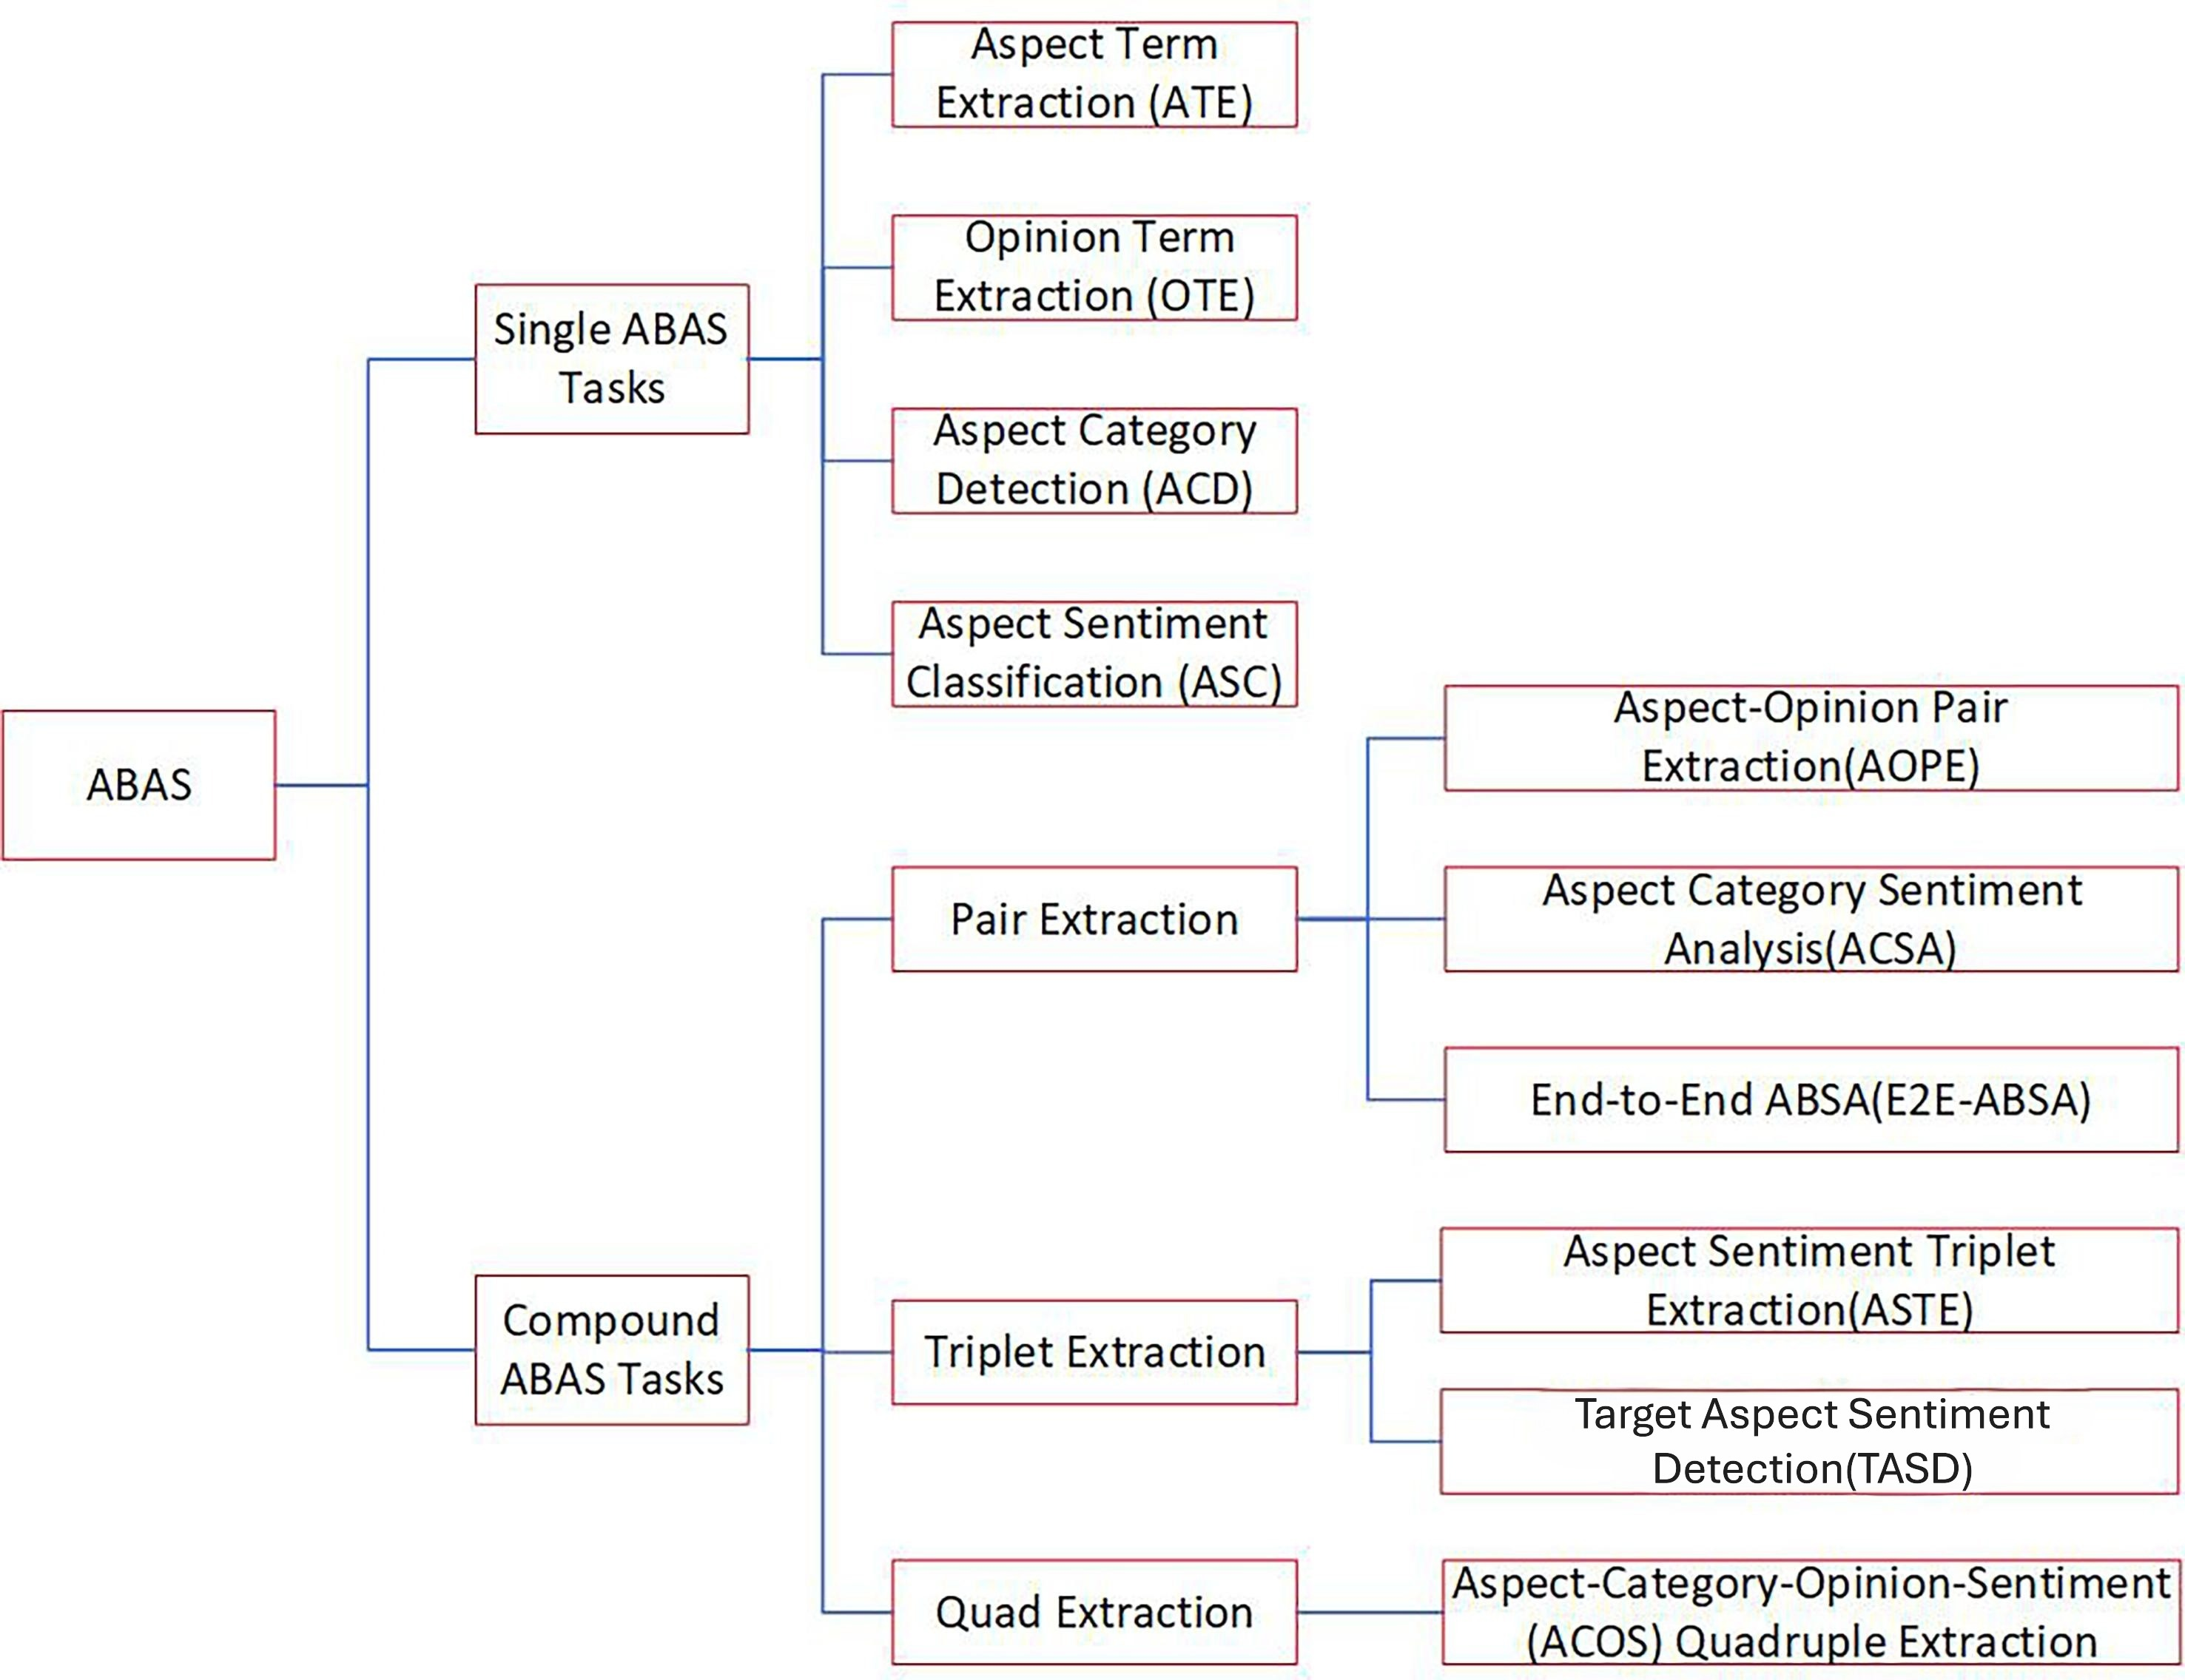
\includegraphics[width=0.9\textwidth]{images/absa}
    \caption[Jednotlivé dílčí úlohy aspektové analýzy sentimentu]%
    {Jednotlivé dílčí úlohy aspektové analýzy sentimentu, upravený obrázek z~\cite{MAO2024102048}}
    \label{fig:ABSA}
\end{figure}
\section{Aspektová analýza sentimentu}\label{absa}
Aspektová analýza sentimentu (ABSA, \emph{Aspect-based sentiment analysis}) je detailní forma analýzy sentimentu, která v poslední době získává významnou pozornost ve výzkumu. Hlavní myšlenkou ABSA je, že emoce nebo názory obsažené v textu se nevztahují pouze na jednu entitu jako celek, ale konkrétně na její určité aspekty či vlastnosti~\cite{TAN2020336}. Výzkum ABSA se obecně zaměřuje na identifikaci sentimentu z několika vzájemně propojených pohledů, zejména na úrovni aspektů, aspektových kategorií, názorových výrazů a polarity sentimentu~\cite{XU2020135}.~\cite{MAO2024102048}

Tato úroveň analýzy sentimentu představuje nejdetailnější stupeň, který lze dále rozčlenit do několika dílčích úloh, zaměřujících se na různé aspekty a jejich vlastnosti. V následujících podsekcích budou nejprve představeny jednotlivé dílčí úlohy aspektové analýzy sentimentu (\emph{Single ABSA Tasks}), a poté budou popsány složitější úlohy (\emph{Compound ABSA Tasks}), vznikající kombinací těchto dílčích úloh, které již poskytují komplexní informace o sentimentu vzhledem k jednotlivým aspektům (viz. Obrázek \ref{fig:ABSA}).

\subsection{Základní dílčí úlohy ABSA}
Aspektová analýza sentimentu zahrnuje čtyři základní dílčí úlohy (tzv. \emph{Single ABSA Tasks}). Konkrétně se jedná o extrakci aspektů (\emph{Aspect Term Extraction, ATE}), extrakci názorových výrazů (\emph{Opinion Term Extraction, OTE}), detekci aspektových kategorií (\emph{Aspect Category Detection, ACD}) a klasifikaci sentimentu aspektů (\emph{Aspect Sentiment Classification, ASC}).~\cite{MAO2024102048}

\begin{itemize}
    \item \textbf{Extrakce aspektů (ATE)} \\
    Cílem této úlohy je identifikace všech aspektů (neboli entit) zmíněných v textu, vůči kterým se následně provádí analýza sentimentu. Jedná se o klíčový krok většiny komplexnějších ABSA úloh, protože definuje hlavní objekty další analýzy.~\cite{zhang2022surveyaspectbasedsentimentanalysis}

    \item \textbf{Extrakce názorových výrazů (OTE)} \\
    Tato úloha spočívá ve vyhledávání slov či frází, které vyjadřují názory nebo postoje, aniž by nutně specifikovaly konkrétní aspekty. Úkolem je tedy získat ze samotného textu výrazy, které se následně přiřazují k relevantním aspektům.~\cite{zhang2022surveyaspectbasedsentimentanalysis}

    \item \textbf{Detekce aspektových kategorií (ACD)} \\
    Tato úloha se věnuje určování obecných kategorií aspektů. Existují zde dva přístupy. První spočívá v kategorizaci aspektů do širších skupin (např. ve větě \uv{Salát byl skvělý, ale náš číšník byl velmi nepříjemný} by výsledkem byly kategorie \uv{jídlo} a \uv{obsluha}~\cite{MAO2024102048}). Druhý přístup využívá kategorie k popisu vlastností jednotlivých aspektů (např. věta \uv{Pokoje jsou skvělé, jsou velmi levné} by vedla ke kategoriím \uv{obecná} a \uv{cena}~\cite{chebolu-etal-2024-oats}).

    \item \textbf{Klasifikace sentimentu aspektů (ASC)} \\
    Tato úloha je přímo zaměřena na určení sentimentu konkrétních aspektů zmíněných v textu. Jde tedy o samotnou analýzu sentimentu, kdy cílem je přiřadit specifikovaným aspektům správnou polaritu sentimentu (pozitivní, negativní či neutrální). Právě tato úloha představuje hlavní zaměření této bakalářské práce.~\cite{zhang2022surveyaspectbasedsentimentanalysis}
\end{itemize}

\subsection{Složené úlohy ABSA}
Jak již bylo zmíněno, složené úlohy ABSA (tzv. \emph{Compound ABSA Tasks}) spojují několik dílčích úloh dohromady, aby bylo možné lépe zachytit a popsat sentiment obsažený v textech. Hlavním cílem těchto úloh je extrahovat a predikovat více sentimentových prvků současně. Mezi typy složených úloh patří extrakce dvojic, trojic a čtveřic sentimentových prvků.~\cite{MAO2024102048}. Jelikož jsou tyto úlohy již nad rámec této práce, budou popsány pouze stručně, podrobnější popis je dostupný v citacích u jednotlivých úloh.

\subsubsection{Extrakce dvojic}
Mezi úlohy založené na extrakci dvojic patří extrakce aspekt-názor dvojic (\emph{Aspect-Opinion Pair Extraction, AOPE}), analýza sentimentu aspektových kategorií (\emph{Aspect Category Sentiment Analysis, ACSA}) a end-to-end aspektová analýza sentimentu (\emph{End-to-End ABSA, E2E-ABSA})~\cite{MAO2024102048}, někdy označovaná jako jednotná aspektová analýza sentimentu (\emph{Unified ABSA, UABSA})~\cite{zhang-etal-2021-towards-generative}. Tyto úlohy poskytují ucelenější pohled na sentiment tím, že spojují jednotlivé prvky analýzy (např. aspekt a odpovídající názor) nebo zároveň určují sentiment vůči daným aspektům.

\begin{itemize}
    \item \textbf{Extrakce aspekt-názor dvojic (AOPE)} \\
    Tato úloha spočívá v extrakci párů tvořených aspektem a k němu náležícím názorovým výrazem. Cílem je identifikovat vazbu mezi konkrétními aspekty a slovy, která je popisují. Například z věty: \uv{Salát byl skvělý a číšník byl také velmi nápomocný} se získají dvojice: \uv{[salát, skvělý]} a \uv{[číšník, nápomocný]}.~\cite{zhang-etal-2021-towards-generative}

    \item \textbf{Analýza sentimentu aspektových kategorií (ACSA)} \\
    Při této úloze se analyzuje sentiment v rámci předem definovaných aspektových kategorií, a tím se určuje celková polarita dané kategorie. Například z věty: \uv{Pití bylo skvělé a jídlo bylo velmi chutné} by se získaly dvojice: \uv{[občerstvení, pozitivní]} a \uv{[občerstvení, pozitivní]}, což dohromady vypovídá o pozitivním sentimentu pro kategorii \uv{občerstvení}.~\cite{li2020multiinstancemultilabellearningnetworks}

    \item \textbf{End-to-End aspektová analýza sentimentu (E2E-ABSA)} \\
    Tato úloha v jednom kroku spojuje extrakci aspektových termínů a jejich klasifikaci sentimentu, tedy zároveň identifikuje aspekty i jejich náladu (polaritu). Například z věty: \uv{Salát byl skvělý a číšník byl také velmi nápomocný} se získají dvojice: \uv{[salát, pozitivní]} a \uv{[číšník, pozitivní]}.~\cite{zhang-etal-2021-towards-generative}
\end{itemize}

\subsubsection{Extrakce trojic}
Mezi úlohy založené na extrakci trojic patří extrakce aspekt-názor-sentiment trojic (\emph{Aspect Sentiment Triplet Extraction, ASTE}) a detekce aspekt-kategorie-sentiment (\emph{Target Aspect Sentiment Detection, TASD}).~\cite{MAO2024102048} Tyto úlohy přinášejí podrobnější popis sentimentu tím, že identifikují nejen aspekty, ale i jejich názory či vlastnosti a sentiment současně.

\begin{itemize}
    \item \textbf{Extrakce aspekt-názor-sentiment trojic (ASTE)} \\
    Cílem této úlohy je identifikovat trojici tvořenou aspektem, k němu příslušným názorovým výrazem a polaritou sentimentu. Poskytuje detailní a přesný vhled do hodnocení, protože zohledňuje, \emph{co} je hodnoceno (aspekt), \emph{jaký} je k němu sentiment a případně \emph{proč} (na základě čeho). Například z věty: \uv{Salát byl skvělý a číšník byl také velmi nápomocný} lze získat trojice: \uv{[salát, skvělý, pozitivní]} a \uv{[číšník, nápomocný, pozitivní]}.~\cite{MAO2024102048, Peng_Xu_Bing_Huang_Lu_Si_2020}

    \item \textbf{Cílená aspektová analýza sentimentu (TASD)} \\
    Tato úloha spočívá v detekci kategorií aspektů, konkrétních aspektů a jejich sentimentové polarity. Hlavním cílem je určit, do jaké kategorie daný aspekt spadá a jakou má polaritu. Například z věty \uv{I přesto, že pizza byla vážně skvělá, cena byla velmi vysoká} lze odvodit trojice: \uv{[pizza, jídlo\#kvalita, pozitivní]} a \uv{[pizza, jídlo\#cena, negativní]}, čímž se vyjádří, že pizza je sice kvalitní, avšak poměrně drahá.~\cite{Wan_Yang_Du_Liu_Qi_Pan_2020, Ke2023}
\end{itemize}

\subsubsection{Extrakce čtveřic}
Nejkomplexnější úlohou v ABSA je extrakce čtveřic, konkrétně jde o extrakci čtveřic aspekt-kategorie-názor-sentiment (\emph{Aspect-Category-Opinion-Sentiment Quadruple Extraction, ACOS})~\cite{MAO2024102048}. Tato úloha integruje všechny základní prvky aspektové analýzy sentimentu a umožňuje nejdetailnější pohled na postoje vyjádřené v textu.

\begin{itemize}
    \item \textbf{Extrakce čtveřic aspekt-kategorie-názor-sentiment (ACOS)} \\
    Tato úloha představuje nejkomplexnější formu extrakce, při které se získávají kompletní čtveřice obsahující konkrétní aspekt, jeho kategorii, odpovídající názor a sentiment. Jako příklad lze uvést větu: \uv{Vypadá pěkně a jeho konstrukce je velice bytelná.} Z této věty je možné získat čtveřice: \uv{[povrch, design, bytelná, pozitivní]} a \uv{[null, design, pěkně, pozitivní]}. V některých případech nemusí být všechny složky čtveřice ve větě explicitně vyjádřeny, což představuje další výzvu této úlohy.~\cite{MAO2024102048, cai-etal-2021-aspect}
\end{itemize}

\subsection{Využití transformátorových modelů v ABSA}
V sekci \ref{TechAnaSen} byly představeny různé metody analýzy sentimentu. Stále více studií se však v současné době zaměřuje na využití transformátorové architektury~\cite{vaswani2023attentionneed}, například modelu BERT~\cite{devlin2019bert} a jeho odvozených variant. Tato část proto popisuje práce, které aplikují BERT na jednotlivé metody ABSA, srovnávají jej s dalšími modely a zkoumají jeho vhodnost v různých doménách i jazycích. Také v této práci budou použity vybrané varianty modelů BERT, a to jak pro různé jazyky, tak pro různé okruhy dat.

\subsubsection{Datasety}
Kvalitní a dostatečně rozsáhlá trénovací data představují klíčový předpoklad úspěchu při trénování modelů. V kontextu analýzy sentimentu, a především u složitějších úloh ABSA, ovšem není dostupných datasetů mnoho. Proto některé studie usilují o tvorbu nových datových sad, jež obsahují větší množství domén, více sentimentů v jedné větě či rozsáhlejší objem dat. Na těchto nových korpusech následně testují výkonnost modelů typu BERT, aby ověřily jejich schopnost zachytit jemné nuance aspektové analýzy.

\begin{itemize}
    \item \textbf{Dataset OATS} \\
    V datové sadě OATS (\emph{Opinion Aspect Target Sentiment})~\cite{chebolu-etal-2024-oats} je cílem připravit objemnější datasety a rozšířit dosavadní spektrum domén (často omezené na recenze notebooků nebo restaurací~\cite{pontiki-etal-2014-semeval}) o další oblasti, jako jsou potraviny (Amazon Food Reviews), online kurzy (Coursera) a hotely (TripAdvisor). Tento dataset je připraven pro několik složených ABSA úloh (E2E-ABSA, ASTE, TASD a ACOS).

    \item \textbf{Dataset MAMS} \\
    Cílem datové sady MAMS (\emph{Multi-Aspect Multi-Sentiment})~\cite{jiang-etal-2019-challenge} je zajistit, aby každá věta obsahovala alespoň dva hodnocené aspekty. Data pocházejí z kolekce CitySearch New York a jsou uzpůsobena primárně pro úlohy E2E-ABSA a ACSA.
\end{itemize}

\subsubsection{Složené úlohy ABSA}
Pro jednotlivé složené úlohy ABSA existuje řada studií, které se zaměřují na hlubší pochopení daných problémů či na formulaci nových variant těchto úloh. V této sekci jsou stručně představeny vybrané práce, jež nabízejí nové pohledy a přístupy.

\begin{itemize}
    \item \textbf{ACSA}
    \begin{itemize}
        \item Jednou z hlavních výzev ACSA je skutečnost, že k jedné kategorii se v jedné větě může vztahovat více názorů. Tento problém řeší například autoři studie~\cite{li2020multiinstancemultilabellearningnetworks}, kteří nejprve vyhledají v textu konkrétní instance aspektových kategorií, přiřadí jim sentiment a následně určí výslednou polaritu pro danou kategorii. 
        
        \item V práci~\cite{LIU2023110339} autoři navrhují model KASA, který tuto úlohu pojímá jako klasifikaci dvojice vět (sentence-pair classification) namísto klasifikace jedné věty (single-sentence classification), čímž ji činí jednodušší k řešení.
    \end{itemize}

    \item \textbf{E2E-ABSA}
    \begin{itemize}
        \item V~\cite{li-etal-2019-exploiting} je popsáno využití modelu BERT a jeho upravených verzí pro End-to-End ABSA. Ve srovnání se staršími modely (např. LSTM) dosahoval BERT výrazně lepších výsledků. Navíc autoři sjednocují porovnání modelů tím, že důsledně využívají samostatný (hold-out) vývojový dataset pro ladění modelu, což dřívější studie často přehlížely. Díky tomu jejich řešení slouží jako BERT-based benchmark pro E2E-ABSA.
    
        \item Autoři studie~\cite{toledo-ronen-etal-2022-multi} se naopak soustředí na vývoj takového modelu pro analýzu sentimentu, který lépe obstojí v různých doménách, a snaží se tak vyřešit problém omezení modelů na konkrétní doménu, jež vyplývá z použití doménově specifických datasetů pro fine-tuning.
    \end{itemize}

    \item \textbf{ASTE}
    \begin{itemize}
        \item Práce~\cite{zhang-etal-2022-boundary} převádí reprezentaci trojic do \uv{relační oblasti} (relation region) v 2D tabulce a pojímá úlohu ASTE jako detekci a klasifikaci těchto oblastí.
        \item Ve studii~\cite{mukherjee-etal-2021-paste} je představen \uv{přístup bez značkování} (tagging-free), který lépe zachycuje vzájemnou závislost mezi komponentami trojice. Autoři využívají architekturu typu encoder-decoder v kombinaci s modelem BERT.
    \end{itemize}

    \item \textbf{TASD}
    \begin{itemize}
        \item Ve studii~\cite{wu2020contextguidedberttargetedaspectbased} autoři rozšiřují BERT o dodatečný kontext a sledují dopady této úpravy na výkonnost modelu. Zároveň poukazují na to, že rozšíření předtrénovaných modelů typu self-attention o kontextové závislosti dokáže významně zlepšit výsledky v kontextově orientovaných jazykových úlohách.
        \item V~\cite{sun-etal-2019-utilizing} se ověřuje, nakolik se zlepší přesnost predikce, pokud je \emph{TASD} pojato jako klasifikace dvojice vět (sentence-pair classification), například formou otázky a odpovědi. Tento přístup je použit i v této práci, kde bude porovnán s klasifikací jedné věty (single-sentence classification).
        \item Někdy aspekt (target) není ve větě explicitně zmíněn, nýbrž pouze naznačen. Příklad: \uv{Jídlo přišlo po 20 minutách a bylo studené.} -- je zde explicitní trojice s aspektem \uv{jídlo}, avšak lze rovněž odvodit negativní hodnocení \uv{obsluhy}, neboť jídlo dorazilo pozdě. Tím se zabývá studie~\cite{Wan_Yang_Du_Liu_Qi_Pan_2020}.
        \item V~\cite{Ke2023} se výzkumníci snaží řešit \emph{TASD} prostřednictvím \uv{systému využívajícího prompty} (prompt-based system), kde je generována otázka a k ní odpověď. Autoři rovněž navrhují vlastní řešení, jak tento přístup aplikovat v praxi.
    \end{itemize}

    \item \textbf{ACOS}
    \begin{itemize}
        \item Ve studii~\cite{cai-etal-2021-aspect} autoři popisují tuto komplexní úlohu, která propojuje všechny dílčí ABSA úlohy, a zároveň vytvářejí datasety Restaurant-ACOS a Laptop-ACOS. Své řešení testují na čtyřech různých systémech, jejichž podrobný popis je uveden v originálním díle.
        \item V~\cite{Li2023-wo} je navržena metoda pro extrakci čtveřic, jež zohledňuje vzdálenost mezi aspekty a názorovými výrazy. Autoři následně porovnávají své výsledky na datasetech Restaurant-ACOS a Laptop-ACOS s jinými přístupy, přičemž dosahují lepších výkonnostních ukazatelů.
    \end{itemize}

\end{itemize}

\section{Využití analýzy sentimentu}
Analýza sentimentu nachází uplatnění v celé řadě oblastí. Díky rozmachu internetu a snadné dostupnosti pro uživatele sdílet své názory a pocity se význam tohoto přístupu neustále zvyšuje. Firmy a organizace mohou na základě recenzí a komentářů efektivně upravovat své produkty a služby, a tím zvyšovat zisk. V oblasti zdravotnictví lze analýzu sentimentu využít například ke sledování potenciálních sebevražedných myšlenek prostřednictvím detekce negativních emocí ve veřejně publikovaných příspěvcích.~\cite{kumar2023comprehensivereviewsentimentanalysis} V následujících podsekcích jsou stručně představeny hlavní oblasti, kde se analýza sentimentu uplatňuje, a uvedeny studie, které se danou tématikou zabývají.

\subsection{Obchodní oblast}
Analýza sentimentu představuje v obchodní sféře jeden z nejvýznamnějších nástrojů pro zlepšování produktů a služeb. Díky schopnosti zpracovat velké množství recenzí lze účinně odhalovat nedostatky a identifikovat příležitosti ke zkvalitnění nabídky. Některé studie~\cite{Sreesurya2020, KUMAR201941} podrobně popisují proces extrakce sentimentu a jeho praktické využití v obchodním prostředí. Další práce se zaměřují na analýzu dat získaných z Amazonu~\cite{BoseSentiment}, z čínských online recenzí~\cite{Wang12022016}, z Facebooku~\cite{Baj-Rogowska} či ze služby Zomato~\cite{9574641}. Souhrnně se těmito tématy zabývají také publikace~\cite{kumar2023comprehensivereviewsentimentanalysis, MAO2024102048, BIRJALI2021107134}.

Analýza sentimentu nemusí sloužit pouze velkým firmám a organizacím, ale nabízí také přínos pro jednotlivce zajímající se o finanční trhy, akcie či kryptoměny. Řada studií~\cite{TadleFOMC, DohHowtoSay, Xing2018} se věnuje využití sentimentu při odhadech vývoje cen akcií a zkoumá, zda pozitivní či negativní nálada může signalizovat budoucí růst nebo pokles. Podobně existují i práce zaměřené na kryptoměny~\cite{ROGNONE2020101462, KRAAIJEVELD2020101188}, které zkoumají, do jaké míry lze sentiment využít pro predikci cenového vývoje. Přehledně se tímto tématem zabývají též díla~\cite{kumar2023comprehensivereviewsentimentanalysis, MAO2024102048, BIRJALI2021107134}.

Analýza sentimentu se nemusí zaměřovat pouze na recenze produktů a služeb, ale lze ji využít i k mapování obecných postojů k aktuálním událostem. Řada studií~\cite{ManguriCovid, NaseemCovid, CHAKRABORTY2020106754, ALAMOODI2021114155, Abd-Alrazaq} například zkoumá reakce uživatelů sociálních sítí (zejména X, původně Twitter) na pandemii COVID-19. Další výzkumy se věnují jiným tématům, jako je rusko-ukrajinská válka~\cite{baker2023prediction} či postoje k elektromobilům v kontextu rostoucích cen pohonných hmot~\cite{JihadEV}. Přehledný souhrn těchto výzkumů nabízejí také články~\cite{kumar2023comprehensivereviewsentimentanalysis, MAO2024102048}.

\subsection{Doporučující systémy}
Analýza sentimentu nachází uplatnění i v doporučujících systémech, ať už jde o hotely či filmy. Typickým přístupem je práce s recenzemi konkrétního uživatele, na jejichž základě lze určit, co by mu mohlo být doporučeno. Různé metody a postupy pro návrh doporučujících systémů popisují studie~\cite{SHEN2019249, LI2016164, SERRANOGUERRERO2020106768, RAY2021106935, FU2020106803}, jejichž souhrn je uveden v~\cite{BIRJALI2021107134}.

\subsection{Zdravotnická oblast}
V předchozích oblastech byla analýza sentimentu popsána především ve vztahu k ekonomickým přínosům, ať už pro firmy nebo pro jednotlivce. Tato metoda však nachází uplatnění i při zlepšování zdravotního stavu populace. Lze ji například využít ke sledování názorů veřejnosti na lékaře, léčiva a zdravotní péči~\cite{JIMENEZZAFRA201950, Ramírez-Tinoco2019, clark2018sentimentanalysisbreastcancer}, nebo k monitorování ohrožených skupin, jako jsou senioři~\cite{Ayata2020}, případně k detekci sebevražedných myšlenek a depresí na základě příspěvků na sociálních sítích~\cite{Desmet2013, Wang2013, Jung2017}. Dokonce existují studie, které se zaměřují na predikci výskytu rakoviny tlustého střeva a konečníku~\cite{Baker2023}. Podrobnější popis uvedených aplikací nabízí např. díla~\cite{kumar2023comprehensivereviewsentimentanalysis, MAO2024102048, BIRJALI2021107134}.

Analýza sentimentu se přitom nemusí týkat pouze fyzického zdraví. Lze ji použít i pro prevenci vulgárních či nenávistných projevů na internetu a tím bránit psychické zdravý online uživatelů. Negativní a urážlivé výrazy mohou u uživatelů vyvolávat stres nebo přispívat k rozvoji depresí. Řada studií se proto zabývá detekcí nenávistných projevů (hate speech) například na X (Twitter)~\cite{Jiang2019, Badjatiya_2017}, Facebooku~\cite{8669073} či analýzou kyberšikany na Instagramu~\cite{Zidny2019}. Souhrnné informace o těchto využitích lze nalézt v~\cite{kumar2023comprehensivereviewsentimentanalysis}.

\section{Otevřené problémy analýzy sentimentu}
Ačkoli se koncept analýzy sentimentu může na první pohled zdát jednoduchý (určitý názor je buď pozitivní, negativní či neutrální), v praxi se často objevují situace, kdy tatáž slova mohou v různém kontextu nést kladný i záporný význam. Člověk tyto nuance rozeznává intuitivně, avšak pro počítačové zpracování představují značnou výzvu. Následující paragrafy nastíní některé z hlavních problémů a otevřených otázek v oblasti analýzy sentimentu. Podrobnější rozbor a další problémy lze nalézt v~\cite{kumar2023comprehensivereviewsentimentanalysis, MAO2024102048, BIRJALI2021107134}.

\paragraph{Sarkasmus}
Sarkasmus se v běžném životě vyskytuje poměrně často, někteří lidé ho používají prakticky denně. Pro klasickou analýzu textu však představuje problém, protože věta, která vypadá na první pohled pozitivně, může být ve skutečnosti míněna ironicky. Různé studie uvedené v~\cite{BIRJALI2021107134} se proto zaměřují na rozpoznávání a správnou interpretaci sarkasmu.

\paragraph{Vícejazyčná analýza sentimentu}
Většina současných výzkumů se soustředí převážně na angličtinu, jelikož pro ni existuje relativně velké množství dat a dalších jazykových zdrojů. U jazyků s nedostatečnou podporou (tzv. \emph{low-resource languages}) je však problematické získat dostatečné datasety pro předtrénování modelů, natož pro samotnou analýzu sentimentu~\cite{BIRJALI2021107134}. Komplikací bývají i texty, v nichž se mísí více jazyků (tzv. \emph{code-switching}), jelikož pro tuto oblast dosud chybějí rozsáhlejší zdroje dat. Podrobnější rozbor těchto obtíží je k dispozici v~\cite{kumar2023comprehensivereviewsentimentanalysis, MAO2024102048, BIRJALI2021107134}.

\paragraph{Problém domén}
Datasety pro trénování analýzy sentimentu obvykle pocházejí pouze z jedné oblasti, například z recenzí notebooků či restaurací~\cite{pontiki-etal-2014-semeval}. Modely se tak naučí rozpoznávat sentiment především v dané doméně, což je nevýhodou při nasazení do jiného kontextu. Některé výrazy, které mají v recenzích notebooků pozitivní význam, se totiž v jiných oblastech nemusí projevovat stejně.~\cite{kumar2023comprehensivereviewsentimentanalysis, MAO2024102048, BIRJALI2021107134}

\chapter{Český jazyk a analýza sentimentu}
Výzkum zpracování přirozeného jazyka se soustředí především na nejčastěji používané jazyky, zejména angličtinu a čínštinu. Tyto jazyky disponují rozsáhlými korpusy, dobře zdokumentovanými benchmarky a nové modely jsou na nich zpravidla validovány jako první (například \emph{ModernBERT}~\cite{warner2024smarterbetterfasterlonger}, který je v době psaní dostupný pouze pro angličtinu).  

U méně rozšířených jazyků, k nimž patří čeština, je situace odlišná. Omezená dostupnost dat, menší komunita a morfologická složitost vedou k nižší míře experimentálního ověřování i praktických aplikací. Tato kapitola proto shrnuje dosavadní práci v oblasti analýzy sentimentu pro český jazyk, popisuje přínos publikovaných studií a diskutuje jejich vliv na další rozvoj metod.

\section{Předešlé práce na analýzu sentimentu v češtině}
Tato sekce se zaměřuje na jednotlivé práce a studie, které se věnují různým aspektům analýzy sentimentu v češtině. Pokrývá témata jako definice sentimentu v českém jazyce, porovnání různých modelů na českých datasetech, představování nových datasetů, a dokonce i vývoj jazykových modelů specializovaných pro češtinu.

\subsection{Problematika analýzy sentimentu v češtině}
V knize~\cite{veselovska-2017} autorka detailně zkoumá problematiku sentimentu v českém jazyce. Popisuje různé jazykové roviny, které byly představeny v sekci~\ref{NLU}, a vysvětluje jejich chování v českém jazyce, přičemž uvádí množství konkrétních příkladů. Také se zaměřuje na emocionální struktury (Formální reprezentace emocionálních struktur), přičemž popisuje jejich analýzu a roli v rámci sentimentu.

Autorka se dále věnuje různým podúkolům. Nejprve zkoumá analýzu sentimentu na větné úrovni v českém jazyce. V této sekci jsou porovnány tři klasifikátory, které jsou testovány na různých datasetech z českých webových stránek.~\cite{veselovska-2017}

Následně se zaměřuje na aspektovou analýzu sentimentu, která využívá dataset SemEval-2014~\cite{pontiki-etal-2014-semeval}, stejně jako v této práci. Avšak \uv{targety} jsou hledány pomocí již známých targetů z trénovacích dat, což znamená, že tento model není dostatečně robustní a nebude fungovat v jiných doménách. Tuto vytvořenou pipeline pak adaptovala i pro češtinu.~\cite{veselovska-2017}

V poslední části autorka popisuje řešení problému TASD v rámci SemEval-2016 Task 5~\cite{pontiki-etal-2016-semeval}. Pro tento úkol byly použity metody hlubokého učení, konkrétně LSTM. Tento přístup vedl k vítězství ve dvou kategoriích (jazycích), ruštině a turečtině. Avšak výsledky nebyly tak uspokojivé v jiných jazycích.~\cite{veselovska-2017}

\subsection{Porovnání různých modelů}
V díle~\cite{_ano_2019} si autoři kladli za cíl provést přehled a porovnání různých tradičních přístupů strojového učení. Použili dva datasety, jeden z Facebooku a druhý z Mall.cz, přičemž se zaměřili pouze na analýzu sentimentu na větné úrovni. Testovali různé modely, jako jsou SVM, logistická regrese (Maximum Entropy) a Naivní Bayes. Dále vyzkoušeli i náhodné lesy a vícevrstvé neuronové sítě. Nejlepší výsledky dosáhl model SVM na datasetu Mall.cz a model logistické regrese na datasetu Facebook.

\subsection{Představení nových technik}
Zajímavý přístup k řešení ACSA předkládají autoři v díle~\cite{priban-prazak-2023-improving}. Spojují dvě úlohy z NLP: aspektovou analýzu sentimentu (ABSA) a sémantické značkování rolí (\emph{Semantic Role Labeling, SRL}). Využívají model ELECTRA~\cite{clark2020electrapretrainingtextencoders}, který je výpočetně méně náročný než modely založené na BERTu. Představují několik způsobů propojení ABSA encoderu a SRL encoderu. V češtině dosáhli zlepšení v obou podúlohách (extrakce kategorií a určení jejich sentimentu), zatímco v angličtině se výsledky nezvýšily -- tam nadále dominují rozsáhlejší modely typu BERT.

\subsection{Datasety v češtině}
Jedním z hlavních úskalí analýzy sentimentu v češtině je omezená dostupnost kvalitních datových sad. Na rozdíl od angličtiny, pro niž existuje rozsáhlé množství datasetů, zůstává čeština podstatně hůře pokryta. Řada studií se proto zaměřuje na tvorbu nových datasetů, jež mají sloužit jako základ pro další rozvoj a zlepšování modelů v českém jazyce. V této části jsou představeny datové sady určené jak pro sentiment na větné úrovni, tak pro aspektovou analýzu sentimentu.

\subsubsection{Analýza sentimentu na větné úrovni}
Tvorbou větně anotovaného datasetu se zabývají autoři v článku~\cite{habernal-etal-2013-sentiment}. Autoři shromáždili příspěvky z devíti českých facebookových stránek a manuálně je označili sentimentem, aby dataset posloužil pro trénink různých modelů. Porovnali výkon SVM a logistické regrese (v článku označované jako \emph{Maximum Entropy}) na vlastním korpusu i na filmových recenzích z ČSFD a produktových recenzích z Mall.cz. Pro každý model otestovali více sad vstupních příznaků a sledovali jejich vliv na přesnost. Výsledky se pohybovaly na podobné úrovni jako ve studii~\cite{_ano_2019}, která s tímto korpusem experimentovala s širším spektrem modelů.

\subsubsection{Aspektová analýza sentimentu}
Ve studii~\cite{steinberger-etal-2014-aspect} autoři představili první český dataset připravený pro ABSA. Korpus vychází z recenzí restaurací, podobně jako dataset SemEval-2014~\cite{pontiki-etal-2014-semeval}, a je anotován pro úlohy ACSA i E2E-ABSA. V této práci bude použit jako jeden z datasetů, na kterých budou natrénovány všechny vybrané modely a následně budou porovnány výsledky mezi češtinou a angličtinou.

Na tento korpus navázala práce~\cite{smid-etal-2024-czech}, jejímž cílem bylo vytvořit dataset pro náročnější úlohy ABSA, konkrétně TASD. Nový dataset byl otestován také na jednodušších úlohách, například ATE, ACD a E2E-ABSA. Autoři se inspirovali strukturou datasetu SemEval-2016~\cite{pontiki-etal-2016-semeval}, který je připraven ve stejném formátu pro více jazyků.

\subsection{České jazykové modely}
Většina nových architektur jazykových modelů je primárně validována na angličtině; vícejazyčné varianty sice později pokrývají až 100 jazyků, avšak jejich kapacita se mezi jazyky dělí nerovnoměrně. Specializované modely trénované čistě na českých datech proto často podávají stabilnější a přesnější výsledky. Následující studie se proto zaměřují na adaptaci vybraných architektur přímo pro češtinu. Všechny zde popsané modely (a další použité v experimentech) jsou podrobněji představené v sekci \ref{Modely}.

\subsubsection{Český BERT -- Czert}
Autoři studie~\cite{sido2021czertczechbertlike} ze Západočeské univerzity vytvořili jazykový model Czert, který je jako první jazykový model natrénovaný výhradně na českých datech. Czert vznikl ve dvou variantách: Czert-B založený na architektuře BERT~\cite{devlin2019bert} a Czert-A vycházející z modelu ALBERT~\cite{lan2020albertlitebertselfsupervised}. V této práci je použita varianta Czert-B, jejíž podrobnější popis lze nalézt v sekci~\ref{Czert}.

\subsubsection{Český RoBERTa -- RobeCzech}
Na Czert navázal model RobeCzech, který využívá architekturu RoBERTa a je rovněž předtrénován na českých datech. Autoři jej otestovali na pěti úlohách včetně analýzy sentimentu a ve všech případech překonal model Czert.~\cite{Straka_2021} Podrobnější popis tohoto modelu lze nalézt v sekci~\ref{RobeCzech}.

\subsubsection{FERNET -- BERT i RoBERTa}
Západočeská univerzita dále publikovala dvojici modelů FERNET (Flexible Embedding Representation NETwork) \cite{Lehe_ka_2021}. První varianta vychází z~BERT-u, druhá z~RoBERTa; obě rozšiřují dostupné české modely a umožňují širší srovnání na domácích datech. Podrobný popis přináší sekce \ref{FERNET}.

\section{Shrnutí dosavadního výzkumu}
Jak ukazuje tento přehled, existuje řada studií zaměřujících se na NLP a analýzu sentimentu v českém jazyce. Tato díla přinášejí užitečné poznatky, ať už v oblasti analýzy sentimentu na větné úrovni, nebo v analýze sentimentu na úrovni aspektů. Většina těchto studií, která porovnává různé modely na různých datasetech, využívá tradiční metody strojového učení, jako jsou SVM, Naivní Bayes nebo logistická regrese. Tyto metody však, ve srovnání s moderními metodami hlubokého učení, konkrétně s transformátorovými modely, vykazují omezenější výkonnost.

Na druhou stranu, novější výzkumy, které se soustředí na tvorbu datasetů a vývoj českých jazykových modelů, se snaží připravit českou komunitu na použití novějších přístupů. Tyto studie nejen že vytvářejí potřebné korpusy pro trénování a testování modelů, ale také otevírají cestu k využívání transformátorových modelů, které jsou schopny efektivněji pracovat s jazykovými nuancemi a hledat ideální řešení pro různé úlohy ABSA. Tento přístup znamená výrazný krok vpřed, protože umožňuje dosáhnout vyšší přesnosti a lepších výsledků na složitějších úlohách analýzy sentimentu.

Tato práce navazuje na poznatky těchto studií a vychází z dosud zpracovaných datasetů pro českou aspektovou analýzu sentimentu. Dále bude využívat český jazykové modely a porovnávat jejich výkon mezi sebou a i s jinými modely, čímž bude přispívat k rozvoji analýzy sentimentu v češtině a hledání ideálních metod pro konkrétní úkoly ABSA.
 
\chapter{Metodologie a postup trénování}
V předchozích kapitolách byly představeny klíčové poznatky z oblasti zpracování přirozeného jazyka, analýzy sentimentu a aspektové analýzy sentimentu. Tato kapitola se soustředí na všechny potřebné kroky nutné k trénování vybraných modelů, a proto zde budou popsány použité datasety, vybrané metody a modely. Dále je detailně vysvětlen postup trénování a představeny vyhodnocovací techniky spolu s praktickými testy modelů.

\section{Datasety}\label{datasety}
Správný výběr dat představuje klíčový faktor pro úspěšné trénování jakéhokoliv modelu, od lineární regrese až po komplexní jazykové modely. Z tohoto důvodu jsou v této práci použity datové sady, které již v angličtině zaznamenaly výraznou pozornost výzkumné komunity. Mezi ně patří dataset SemEval-2014~\cite{pontiki-etal-2014-semeval}, jenž patří k nejčastěji využívaným zdrojům pro ABSA. Pro české prostředí je analogicky použit obdobný dataset recenzí restaurací vytvořený na Západočeské univerzitě~\cite{steinberger-etal-2014-aspect}. Nakonec budou použita také data z archivu Newton Media, která umožní otestovat modely v oblasti mediálních textů.

Každá datová sada je dále popsána samostatně -- nejprve je představen její původ a způsob anotace, následně jsou shrnuty základní statistiky (počet záznamů, průměrná délka textu, distribuce polarit). Součástí popisu je rovněž srovnání různých tokenizátorů: u každého korpusu jsou uvedeny maximální délky tokenizovaných sekvencí, aby byl zřejmý rozdíl mezi tokenizátory trénovanými přímo na jazyku daného datasetu a těmi, které jsou optimalizovány pro jinou jazykovou rodinu. Podle maximální délky je pak vybrané omezení při trénování jednotlivých modelů. Tokenizátory a odpovídající jazykové modely jsou podrobně charakterizovány v sekci \ref{Modely}.

\subsection{Příprava datasetů}
Všechny datasety použité v této práci byly upraveny podle jednotného postupu. Nejprve byly vybrány pouze tři klíčové příznaky: \uv{text}, \uv{aspekt} a \uv{label}. Dataset byl následně očištěn od prázdných hodnot, čímž byla zajištěna kvalita dat pro následné zpracování. Tato práce se zaměřuje na tři hodnoty příznaku \uv{label}, konkrétně na \emph{pozitivní}, \emph{negativní} a \emph{neutrální}. Rozdělení jednotlivých datasetů podle \uv{label} je zobrazeno v grafu~\ref{fig:SentimentDistribution}, který ukazuje i procentuální podíl jednotlivých hodnot \uv{label} v každém z datasetů.

\begin{figure}[ht]\
    \centering
    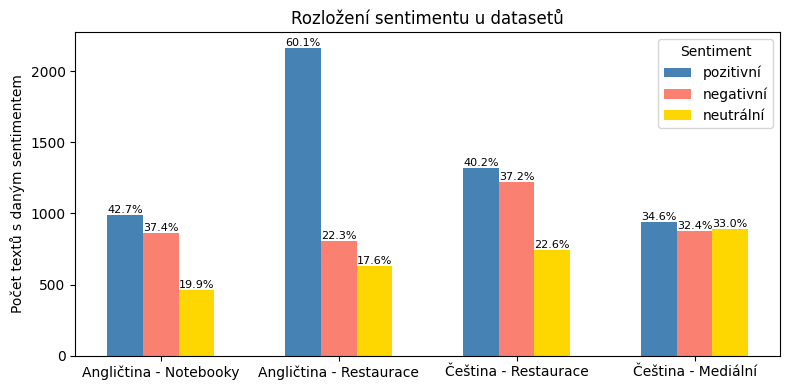
\includegraphics[width=0.9\textwidth]{images/sentiment-distribution}
    \caption[Rozdělení sentimentu v datasetech]%
    {Rozdělení sentimentu v datasetech, vlastní práce}
    \label{fig:SentimentDistribution}
\end{figure}

Pro správné použití datasetů při trénování modelů bylo nejprve nutné každý korpus rozdělit na tři části: \emph{trénovací}, \emph{validační} a \emph{testovací}. Ve všech případech byl zachován jednotný poměr -- 70~\% dat bylo použito pro trénování, 20~\% pro validaci a 10~\% pro závěrečné testování. Předběžné dělení dat zajistí, že všechna následná trénování modelů využijí stejnou strukturu korpusu, a tím umožní objektivně porovnávat dosažené výsledky, protože trénování i vyhodnocení každého modelu proběhne nad totožnými, předem definovanými množinami.

\subsection{Dataset SemEval-2014}
Tato datová sada patřila k prvním, jež se soustředily na aspektovou analýzu sentimentu (ABSA). Do té doby se většina dostupných souborů pro analýzu sentimentu zaměřovala spíše na celkovou náladu či postoj v úrovni celé věty nebo dokumentu. Proto se tým za tímto projektem rozhodl připravit dvě samostatné kolekce recenzí -- jednu zaměřenou na notebooky a druhou na restaurace.~\cite{pontiki-etal-2014-semeval}

Oba datasety byly anotovány dvěma anotátory: jeden byl studentem magisterského studia a druhý odborníkem na lingvistiku. V případě neshod mezi těmito anotátory zasáhl třetí, expertní anotátor. Nejčastější neshody spadaly do jednoho z následujících tří typů: \emph{Nejasnost polarity} (Polarity ambiguity), \emph{Hranice víceslovných aspektů} (Multi-word aspect term boundaries), a \emph{termín aspektu versus odkaz na cílovou entitu} (Aspect term vs. reference to target entity). Podrobnější popis těchto typů a vytváření celého datasetu je uveden v jejich práci~\cite{pontiki-etal-2014-semeval}.

\subsubsection{Recenze notebooků}
Jak již bylo zmíněno, tento dataset byl představen v díle~\cite{pontiki-etal-2014-semeval}. Samotná data však byla získána z portálu Hugging Face, kde je připravil Tom Aarsen a jsou dostupná z~\cite{TomLaptops}.

V datasetu recenzí notebooků je celkem 2313 vzorků, rozdělených na 1619 trénovacích, 462 validačních a 232 testovacích. Tento dataset obsahuje 1456 unikátních textů a 1031 unikátních aspektů. Rozdělení sentimentu v tomto datasetu je znázorněno v grafu~\ref{fig:SentimentDistribution}. Průměrná délka textu činí 104,8 znaků, což odpovídá přibližně 19,3 slovům. Nejdelší text má 464 znaků (nebo 78 slov). Celkové rozložení délky textu je zobrazeno v grafu~\ref{fig:LaptopLenDistribution}.

\begin{figure}[ht]
    \centering
    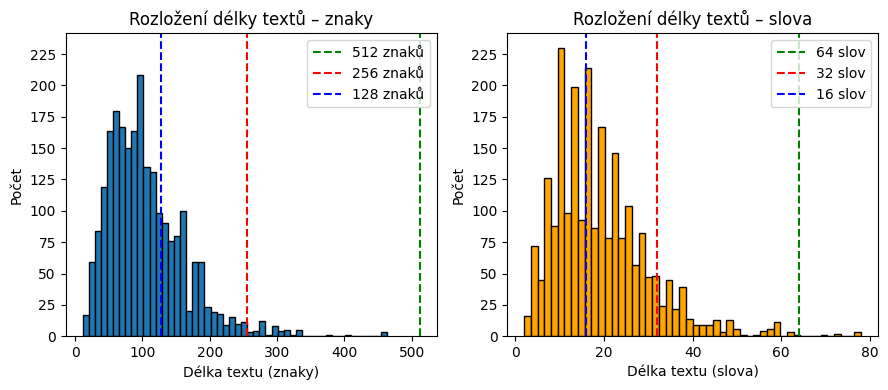
\includegraphics[width=0.9\textwidth]{images/Laptops-distribution}
    \caption[Rozdělení délky textů v datasetu Recenze notebooků v angličtině]%
    {Rozdělení délky textů v datasetu Recenze notebooků v angličtině, vlastní práce}
    \label{fig:LaptopLenDistribution}
\end{figure}

Mezi nejčastější aspekty v tomto datasetu patří: \emph{screen} (obrazovka), \emph{use} (použití) a \emph{price} (cena). Pro tento dataset bylo testováno použití různých tokenizátorů, aby se zjistila ideální délka vstupních sekvencí pro modely. Maximální délky tokenizovaných sekvencí se pohybovaly v rozmezí 97 až 192 tokenů. Tento velký rozptyl je způsoben tím, že na anglický dataset byly použity i tokenizátory, které byly trénovány pouze na češtině, což vedlo k rozdílným výsledkům. Největší rozdíl v délkách tokenizovaných textů je zobrazen v grafu~\ref{fig:LaptopToken}. Podrobné srovnání tokenizátorů bude uvedeno v kapitole~\ref{Results}. Další grafy pro všechny použité tokenizátory a podrobné statistiky tohoto datasetu lze nalézt v souboru \uv{Laptop-English.ipynb}.

\begin{figure}[ht]
    \centering
    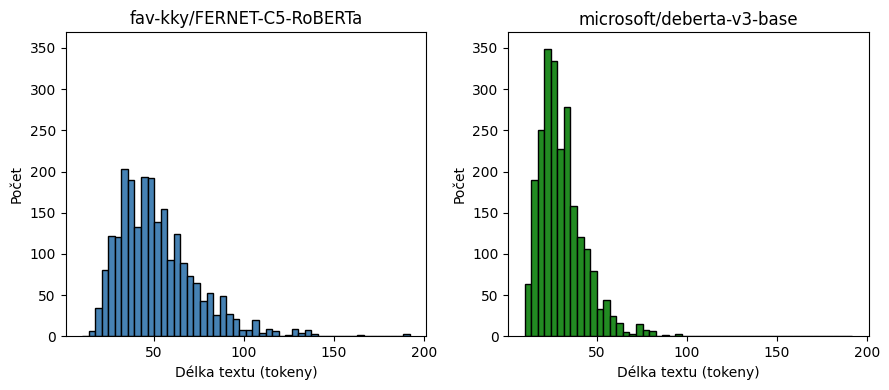
\includegraphics[width=0.9\textwidth]{images/LaptopToken}
    \caption[Porovnání dvou tokenizátorů na datasetu Recenze notebooků v angličtině]%
    {Porovnání dvou tokenizátorů na datasetu Recenze notebooků v angličtině, vlastní práce}
    \label{fig:LaptopToken}
\end{figure}

\subsubsection{Recenze restaurací}
Data pro dataset recenzí restaurací byla také získána z portálu Hugging Face, kde je opět připravil Tom Aarsen, a jsou dostupná z~\cite{TomRestaurants}. Díky tomu, že datasety byly připraveny jedním autorem, je mezi daty zachována konzistence.

Tento dataset obsahuje 3602 vzorků, což ho činí podstatně větším než dataset recenzí notebooků. Vzorky jsou rozděleny na 2521 trénovacích, 720 validačních a 361 testovacích. Tento dataset obsahuje 1976 unikátních textů a 1268 unikátních aspektů. Rozdělení sentimentu v tomto datasetu je zobrazeno v grafu~\ref{fig:SentimentDistribution}. Je zde patrné, že pozitivní data převyšují negativní téměř trojnásobně, což znamená, že modely trénované na těchto datech budou mít tendenci predikovat pozitivní sentiment. Proto se dá předpokládat, že celková přesnost bude výší než u modelů trénovaných na jiných datech. Průměrná délka textu v tomto datasetu je 96,5 znaku, což odpovídá přibližně 17,5 slovům. Nejdelší text má 357 znaků (69 slov). Celkové rozložení délky textu je znázorněno v grafu~\ref{fig:RestaurantLenDistribution}.

\begin{figure}[ht]
    \centering
    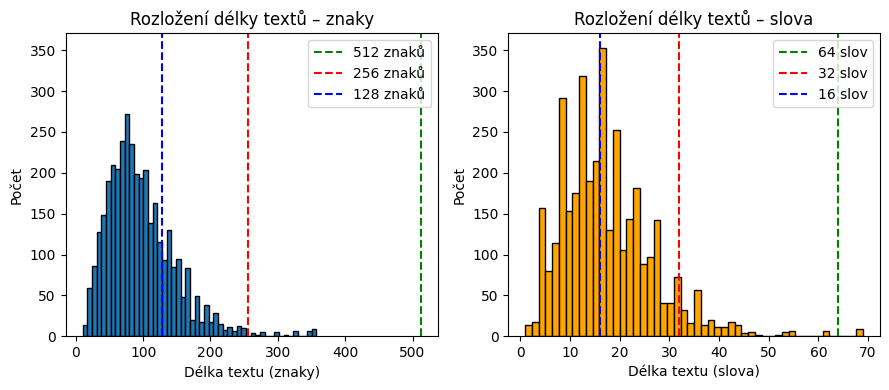
\includegraphics[width=0.9\textwidth]{images/restaurants-distribution}
    \caption[Rozdělení délky textů v datasetu Recenze restaurací v angličtině]%
    {Rozdělení délky textů v datasetu Recenze restaurací v angličtině, vlastní práce}
    \label{fig:RestaurantLenDistribution}
\end{figure}

Mezi nejčastější aspekty v tomto datasetu patří: \emph{food} (jídlo) a \emph{service} (obsluha), které se vyskytují mnohem častěji než ostatní aspekty. Pro zjištění ideální délky vstupů pro model bylo provedeno testování různých tokenizátorů. Maximální délky textů po tokenizaci pro jednotlivé tokenizátory se pohybovaly mezi 90 a 149 tokeny. Zde je opět vcelku velký rozsah maximálních délek, zobrazený v grafu~\ref{fig:RestaurantToken}. Další grafy pro všechny použité tokenizátory a další statistiky týkající se tohoto datasetu jsou k dispozici ve zdrojovém kódu v souboru: \uv{Restaurant-English.ipynb}.

\begin{figure}[ht]
    \centering
    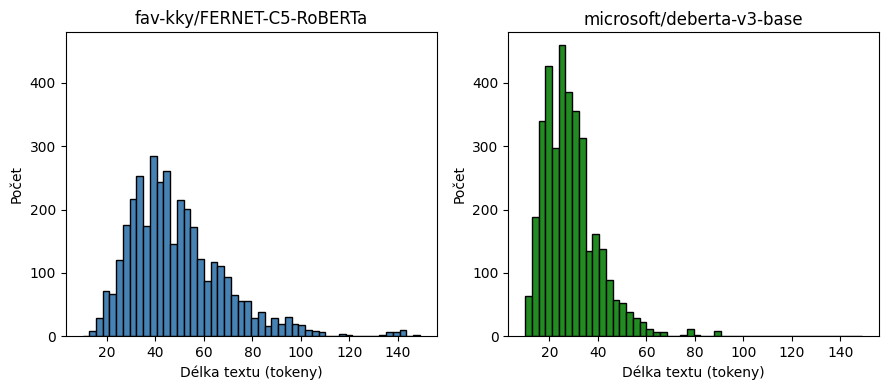
\includegraphics[width=0.9\textwidth]{images/restaurantsToken}
    \caption[Porovnání dvou tokenizátorů na datasetu Recenze restaurací v angličtině]%
    {Porovnání dvou tokenizátorů na datasetu Recenze restaurací v angličtině, vlastní práce}
    \label{fig:RestaurantToken}
\end{figure}

\subsection{Český dataset recenzí restaurací}

Tento dataset vznikl jako česká obdoba datasetu SemEval-2014. Autoři využili recenze restaurací z portálu \url{www.nejezto.cz}, kde vybrali deset podniků s nejvyšším počtem hodnocení. Anotaci provedli tři rodilí mluvčí; podrobnosti o postupu a pravidlech značení jsou popsány v práci~\cite{steinberger-etal-2014-aspect}. Samotná data jsou dostupná v repozitáři~\cite{CzechRestaurants}.

Dataset obsahuje 3281 záznamů, rozdělených na 2296 trénovací, 656 validační a 329 testovací. Z těchto záznamů je 1658 unikátních textů a 1150 unikátních aspektů. Rozdělení polarit sentimentu je zachyceno v grafu~\ref{fig:SentimentDistribution}. Průměrná délka textu činí 124 znaků (přibližně 20,4 slova), nejdelší recenze má 623 znaků (111 slov). Distribuci délek recenzí ukazuje graf~\ref{fig:CzechRestaurantLenDistribution}.

\begin{figure}[ht]
    \centering
    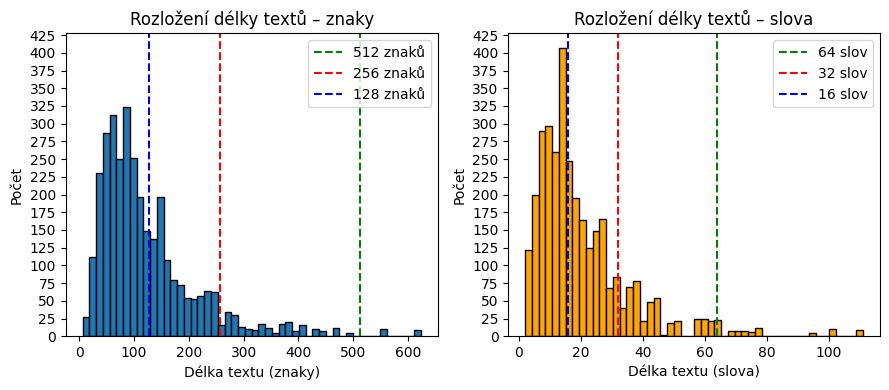
\includegraphics[width=0.9\textwidth]{images/Czechrestaurants-distribution}
    \caption[Rozdělení délky textů v datasetu Recenze restaurací v češtině]%
    {Rozdělení délky textů v datasetu Recenze restaurací v češtině, vlastní práce}
    \label{fig:CzechRestaurantLenDistribution}
\end{figure}

Nejčastěji se v anotacích vyskytují aspekty \emph{jídlo}, \emph{obsluha} a \emph{restaurace}. Mezi deset nejfrekventovanějších patří také tvary \emph{restauraci}, \emph{jídla} či \emph{Jídlo}. Různé pádové tvary ilustrují jednu z komplikací českého jazyka oproti angličtině. Do budoucna by bylo vhodné dataset normalizovat, případně při trénování využít lemmatizaci nebo stemming popsané v sekci~\ref{NLU}.

V tomto datasetu je patrný mnohem větší rozdíl mezi tokenizátory, než v předchozích případech. Maximální délky tokenizovaných sekvencí se pohybovaly v rozmezí od 176 do 358 tokenů. Tento výrazný rozdíl je způsoben tím, že čeština má více znaků, se kterými mají anglické tokenizátory problém. Anglické tokenizátory jsou trénovány primárně na anglických textech a proto mají problém s češtinou, která obsahuje více diakritických znamének a složitější morfologii (např. více pádů). V grafu~\ref{fig:CzechRestaurantToken} je zobrazen největší rozdíl mezi dvěma tokenizátory, který ukazuje tento problém. Grafy pro všechny použité tokenizátory a další statistiky tohoto datasetu jsou k dispozici ve zdrojovém kódu v souboru \uv{Restaurant-Czech.ipynb}.

\begin{figure}[ht]
    \centering
    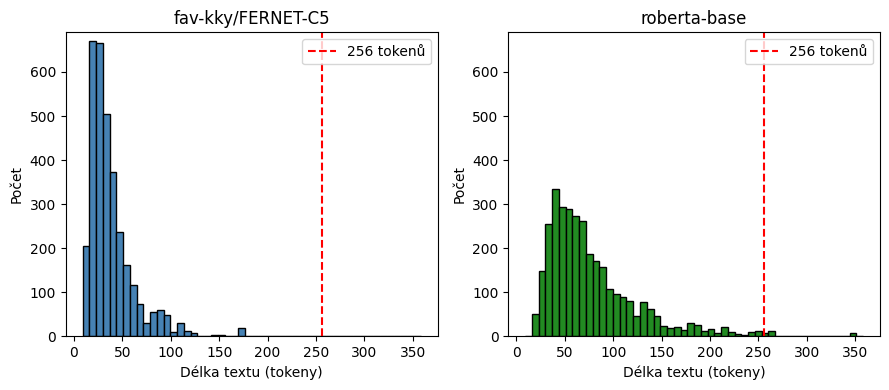
\includegraphics[width=0.9\textwidth]{images/CzechrestaurantsToken}
    \caption[Porovnání dvou tokenizátorů na datasetu Recenze restaurací v češtině]%
    {Porovnání dvou tokenizátorů na datasetu Recenze restaurací v češtině, vlastní práce}
    \label{fig:CzechRestaurantToken}
\end{figure}

\subsection{Data z mediální domény}\label{datasetmedia}
Původně měla být použita reálná data z archivu Newton Media. Analýza však ukázala, že dostupné korpusy jsou pro trénování jazykových modelů nevhodné -- anotace aspektů jsou nevyvážené a počet tříd výrazně kolísá. Proto byl vytvořen \emph{syntetický} dataset, který byl následně použit pro trénování modelů.

\subsubsection{Popis generování dat}
Data byla vygenerována pomocí modelu Gemini 2.0 Flash~\cite{Gemini}. Proces generování probíhal tak, že z reálných článků byly nejprve vybrány tři nejdůležitější aspekty. Každému z těchto aspektů byl následně přiřazen náhodný sentiment. Poté bylo vytvořeno shrnutí daného článku, přičemž byl kladen důraz na zachování přiřazeného sentimentu k daným aspektům. K extrakci aspektů byl použit prompt uvedený v~\ref{code:prompt}. Pro generování shrnutí s konkrétním sentimentem k těmto aspektům byl následně použit druhý prompt, uvedený v~\ref{code:prompt2}. Přesné použití těchto promptů a celý proces generování lze nalézt v příloze v souboru \uv{script.py}.

\begin{listing}[ht]
\begin{minted}{python3}
f"""Najdi {n} nejdůležitějších, vzájemně odlišných aspektů, 
které se týkají hlavního tématu následujícího textu. Aspekt je 
jednoduché podstatné jméno nebo fráze, která popisuje konkrétní 
vlastnost nebo aspekt daného tématu. Například: „kvalita 
produktu“, „cena“, „zákaznický servis“.
Napiš seznam aspektů, které jsou relevantní pro daný text. 
Nepoužívej žádné úvodní fráze ani vysvětlení, pouze seznam 
aspektů.""""
\end{minted}
\caption[Ukázka promptu pro extrakci nejdůležitějších aspektů]%
{Ukázka promptu pro extrakci nejdůležitějších aspektů, vlastní práce}
\label{code:prompt}
\end{listing}

\begin{listing}[ht]
\begin{minted}{python3}
f"""Následující text se týká několika aspektů: {aspects_repr}.
Napiš souvislé shrnutí (max 200 slov), kde každý aspekt je 
zmíněn a popsán tónem, který mu byl přiřazen (pozitivní/
negativní/neutrální). Snaž se o obecné shrnutí, kde jsou 
aspekty mimochodem zmíněny.
Nezapomeň na žádný aspekt a dbej, aby výsledný odstavec působil 
přirozeně. Pamatuj, že to má být shrnutí, ne analýza! I kdyby 
byl aspekt v textu zmíněň například s jiným tónem než zadáno, 
shrnutí by mělo být v souladu s tónem zadaným v úkolu a nikoli 
s tónem v textu.""""
\end{minted}
\caption[Ukázka promptu pro generaci shrnutí]%
{Ukázka promptu pro generaci shrnutí, kde se dbá na daný sentiment k daným aspektům, vlastní práce}
\label{code:prompt2}
\end{listing}

\subsubsection{Popis samotného datasetu}
Po finálních úpravách obsahuje dataset 2709 záznamů, rozdělených na 1896 trénovacích, 542 validačních a 271 testovacích instancí. Celkem zahrnuje 903 unikátních textů a 1681 aspektů. Polaritní rozložení je vyvážené (graf~\ref{fig:SentimentDistribution}), což eliminuje zkreslení při trénování modelů. Průměrná délka textu činí 529,2 znaku, přibližně 75,5 slova, nejdelší text dosahuje 862 znaků (125 slov). Distribuci délek ukazuje graf~\ref{fig:CzechMediaLenDistribution}. Oproti předchozím datasetům jsou texty podstatně delší, což odpovídá charakteru mediálních článků.

\begin{figure}[ht]
    \centering
    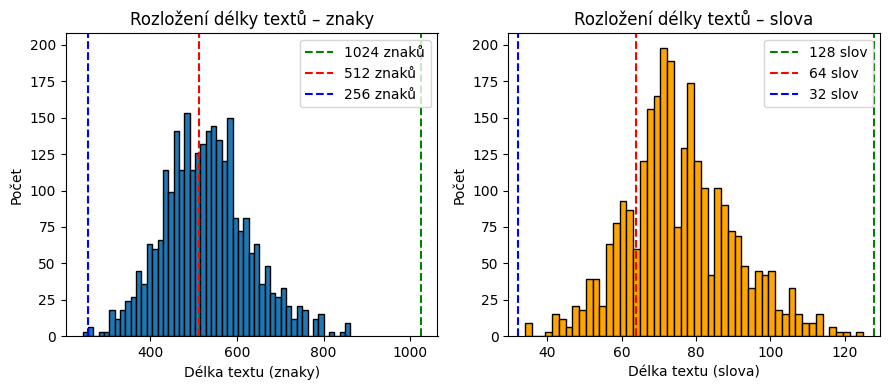
\includegraphics[width=0.9\textwidth]{images/Czechmedia-distribution}
    \caption[Rozdělení délky textů v datasetu Mediální texty v češtině]%
    {Rozdělení délky textů v datasetu Mediální texty v češtině, vlastní práce}
    \label{fig:CzechMediaLenDistribution}
\end{figure}

Nejfrekventovanějšími aspekty v celém korpusu jsou \emph{coming out}, \emph{dlouholetý vztah} a \emph{příčina výpadku}; žádný z nich však nevyčnívá svou absolutní četností natolik, aby převážil nad ostatními. V tomto datasetu je rozdíl mezi tokenizátory ještě výraznější než u dříve popsaných sad -- maximální délky tokenizovaných sekvencí se pohybovaly od 170 do 482 tokenů. Graf~\ref{fig:CzechMediaToken} ukazuje kontrast mezi dvojicí tokenizátorů stejné architektury RoBERTa~\cite{liu2019robertarobustlyoptimizedbert}: česká varianta dosahuje svých nejdelších sekvencí přibližně na úrovni nejkratších sekvencí anglické verze, což dokládá, že anglické tokenizátory si s češtinou poradí podstatně hůře. Další grafy délek po tokenizaci a doplňkové statistiky k tomuto korpusu jsou k dispozici v přiloženém notebooku \uv{Media‑Czech.ipynb}.

\begin{figure}[ht]
    \centering
    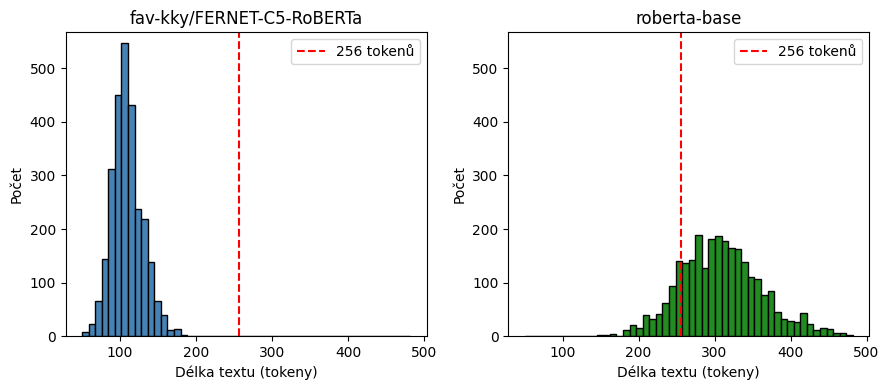
\includegraphics[width=0.9\textwidth]{images/CzechmediaToken}
    \caption[Porovnání dvou tokenizátorů na datasetu Mediální texty v češtině]%
    {Porovnání dvou tokenizátorů na datasetu Mediální texty v češtině, vlastní práce}
    \label{fig:CzechMediaToken}
\end{figure}

\section{Vybrané metody}\label{VybMet}
Využití BERT modelů pro ABSA se zabývali autoři článku~\cite{sun-etal-2019-utilizing}, kteří představili čtyři nová řešení zaměřená specificky na TASD a E2E-ABSA. Využívají vlastnost modelu BERT, konkrétně jeho struktura vstupu, díky čemuž je možné převést úkoly ABSA (ať už jakékoliv podúlohy) na klasifikaci dvojice vět (\emph{sentence-pair classification}). Tento přístup bude testován i v této práci, kde bude porovnávána klasifikace dvojice vět s klasifikací jedné věty (\emph{single-sentence classification}).

Při převodu ABSA úloh na klasifikaci dvojice vět se druhá věta používá jako doplňující informace k získání sentimentu z původního textu. Jedna věta je původní text a druhá slouží jako doplňující (\emph{auxiliary sentence}). Tato pomocná věta může být formulována buď jako otázka (\emph{QA}), nebo jako pseudo-věta (\emph{NLI}). Tyto dva přístupy se pak dále dělí podle toho, zda bude odpovědí polarita sentimentu (\emph{M}), nebo odpověď typu ano/ne (\emph{B})~\cite{sun-etal-2019-utilizing}.
\begin{itemize}
    \item \textbf{QA-M} \\
    Doplňující věta je ve formě otázky, na kterou bude odpověď už daná polarita sentimentu. Příklad otázky: \uv{Jaký je sentiment tohoto aspektu: \{aspect\}?}, kde za \{aspect\} může být dosazen libovolný požadovaný aspekt z daného textu.
    \item \textbf{NLI-M} \\
    Doplňující věta v tomto případě nemá přísná pravidla a jedná se o tzv. pseudo-větu. Může jít například o větu jako: \uv{aspekt: \{aspect\}}. Model pak vrací polaritu sentimentu na základě této věty.
    \item \textbf{QA-B} \\
    Doplňující věta je opět ve formě otázky, ale úloha je převedena na binární odpověď (ano/ne). Polarita sentimentu může mít tři možné hodnoty: \uv{pozitivní}, \uv{negativní} a \uv{neutrální}. V této metodě je třeba vygenerovat tři různé otázky pro jeden text, což znamená, že predikce musí být provedena třikrát, aby byly získány odpovědi pro všechny tři polarity. Příklad možných otázek: \uv{Je sentiment pro aspekt: \{aspect\} pozitivní?}, \uv{Je sentiment pro aspekt: \{aspect\} negativní?} a \uv{Je sentiment pro aspekt: \{aspect\} neutrální?}.
    \item \textbf{NLI-B} \\
    Opět jde o pseudo-větu, která však již obsahuje informaci o sentimentu. Opět bude potřeba vygenerovat tři věty pro jeden text. Příklad takových vět: \uv{aspekt: \{aspect\}, sentiment: pozitivní}, \uv{aspekt: \{aspect\}, sentiment: negativní}, \uv{aspekt: \{aspect\}, sentiment: neutrální}.~\cite{sun-etal-2019-utilizing}
\end{itemize}

Jak již bylo zmíněno, v této práci budou použity dvě metody: jedna pro klasifikaci jedné věty a druhá pro klasifikaci dvojice vět. Pro klasifikaci dvojice vět bude z metod popsaných výše vybrána metoda \emph{QA-M}. Tato metoda byla zvolena na základě pozorování v práci~\cite{sun-etal-2019-utilizing}, která ukázala, že metody typu \emph{QA} dosahovaly lepších výsledků při predikci sentimentu. Verze \emph{M} byla vybrána kvůli její jednoduchosti a menší náročnosti na trénování (u verze \emph{B} by trénování trvalo třikrát déle). Popis implementace těchto metod bude uveden v sekci~\ref{PristupToken}.

\section{Vybrané modely}\label{Modely}
Tato část představuje všechny modely testované v rámci této práce a vysvětluje jejich rozdělení do dvou logických skupin. Mezi nimi bude vybírán nejvhodnější kandidát pro český mediální prostor a na každý z nich se aplikují obě metody popsané v sekci~\ref{VybMet}. Všechny modely jsou založeny na transformátorové architektuře a vycházejí z modelu BERT, který je rovněž součástí této práce.

Modely jsou rozděleny na \emph{inovativní} a \emph{jazykově adaptované}. První skupinu tvoří architektury, které přinášejí nové předtrénovací postupy či mechanismy (např.\ RoBERTa, DeBERTa-V3, ModernBERT). Do druhé skupiny patří verze již existujících modelů přetrénované pro konkrétní jazyková prostředí, zejména pro češtinu a další slovanské jazyky (SlavicBERT, Czert, RobeCzech, FERNET).

Pro popis těchto modelů jsou používány následující parametry: \emph{počet vrstev L} (počet transformátorových bloků), \emph{velikost skrytého vektoru H} (velikost vektoru, který reprezentuje jednotlivé tokeny v každé vrstvě transformátoru) a \emph{počet self-attention hlav A} (počet nezávislých mechanismů pozornosti, které model používá k výpočtu pozornosti pro každý token vzhledem k ostatním tokenům)~\cite{devlin2019bert}. Vypsané parametry všech modelů lze nalézt v tabulce~\ref{tab:modely}.

\begin{table}[ht]
    \centering
    \begin{tabular}{|l|c|c|c|c|}
        \hline
        \textbf{model} & \textbf{L} & \textbf{H} & \textbf{A} & \textbf{počet parametrů}  \\ \hline
        bert-base-uncased & 12 & 768 & 12 & 110 milionů \\ \hline
        bert-large-uncased & 24 & 1024 & 16 & 340 milionů \\ \hline
        bert-base-multilingual-cased & 12 & 768 & 12 & 110 milionů \\ \hline
        roberta-base & 12 & 768 & 12 & 125 milionů \\ \hline
        xlm-roberta-base & 12 & 768 & 12 & 270 milionů \\ \hline
        xlm-roberta-large & 24 & 1024 & 16 & 550 milionů \\ \hline
        deberta-v3-base & 12 & 768 & 12 & 184 milionů \\ \hline
        ModernBERT-base & 22 & 768 & 12 & 149 milionů \\ \hline
        ModernBERT-large & 28 & 1024 & 16 & 395 milionů \\ \hline\hline
        bert-base-bg-cs-pl-ru-cased & 12 & 768 & 12 & 180 milionů \\ \hline 
        Czert-B-base-cased & 12 & 768 & 12 & 110 milionů \\ \hline
        robeczech-base & 12 & 768 & 12 & 126 milionů \\ \hline
        FERNET-C5 & 12 & 768 & 12 & 164 milionů \\ \hline
        FERNET-C5-RoBERTa & 12 & 768 & 12 & 124 milionů \\
        \hline
    \end{tabular}
    \caption{Parametry použitých modelů}
    \label{tab:modely}
\end{table}

\subsection{Inovativní modely}
Následující podsekce popisují modely, které posouvají možnosti transformátorových architektur prostřednictvím nových trénovacích technik, modifikované pozornosti či efektivnější implementace. Tyto inovace mají za cíl zvýšit přesnost, zrychlit rozhodování a snížit paměťové nároky, což je klíčové zejména při zpracování rozsáhlých textových korpusů.

\subsubsection{BERT}
Model BERT (zkratka pro \emph{Bidirectional Encoder Representations from Transformers}) byl představen v práci~\cite{devlin2019bert} jako řešení pro široké spektrum úloh na úrovni věty a tokenu (sentence-level and token-level tasks). Předchozí modely byly zaměřeny pouze na jeden směr čtení textu, zatímco BERT, díky své \emph{dvojcestné} (bidirectional) architektuře, dokáže zohlednit kontext z obou stran textu, což zlepšuje predikci tokenů. BERT je předtrénovaný model, který se nejprve trénuje na obecných datech a poté je možné jej doladit (fine-tune) na specifických úlohách s menšími datovými sadami.

BERT je postaven na transformátorové architektuře, která byla představena v sekci~\ref{Transformator}, využívající model encoder, popsán v sekci~\ref{DECENC}. Vstupy do modelu BERT mohou být jak jednotlivé věty, tak dvojice vět (například otázka a odpověď). Tato flexibilita rozšiřuje možnosti využití modelu, jak je tomu i v této práci. Pro předtrénování modelu BERT byly použity dva rozsáhlé datasety: BooksCorpus (800 milionů slov) a anglická Wikipedie (2,5 miliardy slov). Předtrénovací techniky zahrnovaly \emph{Missing token prediction} a \emph{Next sentence prediction}, které jsou podrobněji popsány v sekci~\ref{predtrenovani}. Podrobnější popis modelu BERT lze nalézt v díle~\cite{devlin2019bert}.

V této práci byly použity dvě verze modelu BERT: \emph{bert-base-uncased}~\cite{BERTbaseuncased} a \emph{bert-large-uncased}~\cite{BERTlargeuncased}. Jedná se o stejné modely, lišící se pouze velikostí. Větší modely jsou schopny zachytit složitější vlastnosti textu, ale jsou výpočetně náročnější.~\cite{devlin2019bert} Zvoleny byly \emph{uncased} verze, protože patří k nejpoužívanějším anglickým modelům BERT a v praxi se nasazují častěji než jejich \emph{cased} protějšky (\emph{bert-base-cased}~\cite{BERTbasecased} a \emph{bert-large-cased}~\cite{BERTlargecased}).

\subsubsection{mBERT}
Model \emph{multilingual BERT} (mBERT) vychází ze stejné architektury jako původní anglický BERT; liší se pouze trénovacími daty. Byl trénován na Wikipediích ve 100 jazycích s největším počtem článků. Rozložení dat mezi jazyky je však nerovnoměrné -- například angličtina tvoří přibližně 21~\% veškerých trénovacích dat. Aby i jazyky s omezenými zdroji (\emph{low-resource} jazyky) získaly dostatečné zastoupení, autoři použili vyvážené vzorkové (sample) schéma. Podrobné informace jsou uvedeny v repozitáři projektu~\cite{GoogleResearchGitHubMulti}.

mBERT nemá \emph{large} variantu, proto je v této práci použit model \emph{bert-base-multilingual-cased}~\cite{mBERTbasecased}. Verze \emph{cased} je doporučena tvůrci modelu, protože opravuje normalizační problémy u mnoha jazyků, speciálně je doporučena pro jazyky, které nepoužívají latinku (většinou je lepší i pro jazyky, které latinku používají).~\cite{GoogleResearchGitHubMulti}

\subsubsection{RoBERTa}
Model RoBERTa (\emph{Robustly Optimized BERT Pretraining Approach}) vznikl na základě zjištění, že původní BERT je ve fázi předtrénování nedostatečně využit. Autoři proto navrhli několik úprav předtrénovacího postupu:

\begin{enumerate}
    \item delší trénování na rozsáhlejších datech,
    \item odstranění \emph{Next Sentence Prediction},
    \item trénování na delších sekvencích,
    \item dynamickou změnu maskovacího vzoru v průběhu trénování.
\end{enumerate}

Díky uvedeným úpravám dosahuje RoBERTa ve srovnání s původním modelem BERT-em výrazně lepších výsledků napříč různými jazykovými úlohami. Podrobné zdůvodnění jednotlivých vylepšení a jejich vliv na výkon modelu je rozebráno v původním článku~\cite{liu2019robertarobustlyoptimizedbert}.

V této práci je použit model \emph{roberta-base}~\cite{RoBERTabase}. RoBERTa se nečlení na varianty \emph{cased} a \emph{uncased}, takže nebylo nutné volit mezi různými verzemi.

\subsubsection{XLM-RoBERTa}
XLM-RoBERTa je vícejazyčný model navržený jako nástupce mBERT pro vícejazyčné úlohy. Vznikl kombinací optimalizovaného předtrénovacího postupu z modelu RoBERTa a techniky předtrénování XLM (\emph{cross-lingual language models}, vícejazyčné jazykové modelování) představené v práci~\cite{lample2019crosslinguallanguagemodelpretraining}. Výsledkem je model schopný pracovat se 100 jazyky, který překonává předešlé nejlepší modely. Podrobnosti o architektuře a trénování jsou popsány v~\cite{conneau2020unsupervisedcrosslingualrepresentationlearning}.

V této práci jsou použity obě dostupné velikosti: \emph{xlm-roberta-base}~\cite{XLMRoBERTabase} a \emph{xlm-roberta-large}~\cite{XLMRoBERTalarge}. Jde o jediný vícejazyčný model v této práci, který je k dispozici i ve variantě \emph{large}.

\subsubsection{DeBERTa-V3}
Modelová architektura DeBERTa (\emph{Decoding-enhanced BERT with disentangled attention}) rozšiřuje možnosti BERT a RoBERTa dvěma hlavními inovacemi. První z nich je rozdělená pozornost (\emph{disentangled attention}): každé slovo je reprezentováno dvojicí vektorů -- jeden nese obsahovou informaci, druhý relativní pozici -- a váhy pozornosti se počítají odděleně pro obsahové a polohové složky. Druhou novinkou je vylepšený maskovací dekodér, jenž do předtrénování začleňuje i absolutní pozice tokenů. Podrobnosti těchto inovací uvádí práce~\cite{he2021debertadecodingenhancedbertdisentangled}.

Tato práce využívá novější variantu \emph{DeBERTa-V3}, jež nahrazuje klasickou techniku předtrénování predikce chybějícího tokenu (\emph{missing token prediction}) technikou predikce vyměněného tokenu (\emph{replaced token detection}). Také je zde představena nová metoda \emph{gradient-disentangled embedding sharing}, která zlepšuje efektivnost trénování a celkovou kvalitu modelu. Při stejném předtrénovacím režimu jako původní DeBERTa tato vylepšení ukazují zlepšení na širokém spektru NLU úloh. Podrobnější popis těchto vylepšení lze nalézt v díle~\cite{he2023debertav3improvingdebertausing}.

Použitým modelem je \emph{deberta-v3-base}~\cite{DeBERTav3base}. Existuje i vícejazyčná varianta mDeBERTa-V3, ta však pokrývá pouze 16 jazyků a čeština mezi nimi chybí, proto není v této práci použita.

\subsubsection{ModernBERT}
ModernBERT představuje nejnovější encoder-only model vycházející z původního BERT-u. Autoři do klasické transformátorové architektury postupně začlenili řadu ověřených novinek a přidali vlastní úpravy zaměřené na efektivitu jak z hlediska rychlosti, tak paměťové náročnosti. Současně optimalizovali implementaci pro trénování na GPU. Podrobný popis všech změn je uveden v práci~\cite{warner2024smarterbetterfasterlonger}.

Ve srovnání s dřívějšími modely (např. DeBERTa) je ModernBERT výrazně úspornější a typicky alespoň dvakrát rychlejší; v některých úlohách autoři uvádějí až čtyřnásobné zrychlení při současném snížení paměťových nároků. Další zásadní předností je maximální kontextová délka 8192 tokenů, tedy téměř šestnáctinásobek běžného limitu 512 tokenů. Přehled měřených vlastností a praktická srovnání shrnuje blogový článek~\cite{modernbertreplacment}.

V této práci jsou otestovány obě velikosti modelu, \emph{ModernBERT-base}~\cite{ModernBERTbase} a \emph{ModernBERT-large}~\cite{ModernBERTlarge}. Vícejazyčná varianta zatím neexistuje; kdyby byla k dispozici, nabízela by ideální kombinaci dlouhého kontextu a mnohojazyčné podpory pro analýzu rozsáhlých mediálních textů.

\subsection{Jazykově adaptované modely}
Tato podsekce se věnuje variantám, které nepřinášejí nové architektonické prvky, ale rozšiřují stávající modely na méně zastoupené jazyky -- zde především na češtinu a další slovanské jazyky. Jejich hlavním přínosem je tedy jazyková adaptace, využívají osvědčené inovace z předchozí skupiny a převádějí je do jazykového prostředí, kde původní anglické a vícejazykové modely nedosahují optimální výkonnosti.

\subsubsection{SlavicBERT}
SlavicBERT patří mezi první specializované varianty BERT-u zaměřené na slovanské jazyky (češtinu, ruštinu, polštinu a bulharštinu). Autoři vyšli z modelu \emph{mBERT} a dále jej doladili na korpusech výhradně v těchto čtyřech jazycích, protože trénovat novou architekturu od začátku by bylo výpočetně i finančně nákladné. Původně byl model navržen pro rozpoznávání vícejazyčných pojmenovaných entit (NER, named entity recognition), nicméně je použitelný i pro další úlohy zpracování přirozeného jazyka~\cite{arkhipov-etal-2019-tuning}.

V této práci je využita verze \emph{bert-base-bg-cs-pl-ru-cased}~\cite{SlavicBERThug}, která je na portálu Hugging Face dostupná jako jediná oficiálně zveřejněná varianta.

\subsubsection{Český BERT -- Czert}\label{Czert}
Cílem autorů modelu Czert bylo vytvořit model vycvičený výhradně na českých datech. Na rozdíl od SlavicBERT-u zvolili trénování \emph{od nuly}, aby se model učil jazyk čistě z českého korpusu. K předtrénování použili přibližně 36 GB textu. Architektura i postup kopírují původní BERT, jedinou úpravu vyžadovala technika \emph{Next Sentence Prediction}: vzhledem ke krátkým textovým blokům často chyběla vhodná následující věta, což autoři řešili v detailech popsaných v práci~\cite{sido2021czertczechbertlike}.

Vznikly dvě varianty: \emph{Czert-B} založená na BERT-u a lehčí \emph{Czert-A} vycházející z ALBERT-u. Pro tuto práci je zvolen model \emph{Czert-B-base-cased}~\cite{CzertHugging}, jehož rozměry odpovídají mBERT-u a usnadňují tak férové porovnání s ostatními modely.

\subsubsection{Český RoBERTa -- RobeCzech}\label{RobeCzech}
Na dosavadní český model založený na architektuře BERT (Czert) navázal model RobeCzech, jenž vychází z architektury RoBERTa. Předtrénování proběhlo na souboru českých korpusů o celkovém rozsahu převyšujícím čtyři miliardy tokenů a k tréninku byl použit oficiální kódový rámec pro RoBERTa. Následně byl RobeCzech doladěn a vyhodnocen na pěti úlohách z oblasti NLP, mezi nimiž byla i klasická (ne-aspektová) analýza sentimentu. Ve všech sledovaných úlohách překonal ostatní modely stejné velikostní kategorie. Podrobný popis korpusu, parametrů trénování i výsledků benchmarku je uveden v práci~\cite{Straka_2021}.

V této práci se používá \emph{robeczech-base}~\cite{RobeCzech}; jedná se o jedinou dosud publikovanou varianta tohoto modelu, další verze zatím nebyly vytvořeny.

\subsubsection{Český BERT a RoBERTa -- FERNET}\label{FERNET}
Název FERNET zastřešuje dvojici českých modelů, jejichž cílem bylo rozšířit portfolio dostupných jazykových modelů pro češtinu. Autoři zvolili jiné předtrénovací korpusy než u předchozích modelů Czert a RobeCzech -- konkrétně vlastní korpusy \emph{Czech News} a \emph{C5}, jenž představuje českou obdobu anglického C4~\cite{JMLR:v21:20-074}. Na těchto datech vznikly dvě varianty: \emph{FERNET-C5}, vycházející z architektury BERT, a \emph{FERNET-News}, založená na architektuře RoBERTa. Oba modely byly po jemném doladěním srovnány na dvou úlohách z oblasti NLP, z nichž jedna byla opět klasická analýza sentimentu; v tomto srovnání dosáhl FERNET-C5 nejlepších výsledků mezi dostupnými českými modely. Detailní popis přípravy dat, parametrů trénování a dosažených skóre přináší studie~\cite{Lehe_ka_2021}.

V této práci budou využity dvě varienty: \emph{FERNET-C5}~\cite{FERNET-C5} a \emph{FERNET-C5-RoBERTa}~\cite{FERNET-C5-RoBERTa}. Druhý model, ačkoli nebyl součástí původního článku, je model založený na architektuře RoBERTa, který byl předtrénován jak na datasetu C5, tak na datasetu českých novinek.

\section{Popis přístupu}
V předchozích částech byly podrobně představeny použité datasety, metody i jazykové modely. Tato sekce vysvětluje, \emph{jak} byly všechny tyto komponenty propojeny v praxi. Popisuje trénovací prostředí, klíčové knihovny a důležité fragmenty kódu, které zajišťují trénování a vyhodnocení modelů.

\subsection{Trénovací prostředí}
Veškeré trénování probíhalo v prostředí Google Colab \cite{GoogleColab} -- hostovaném Jupyter notebooku -- který poskytuje zdarma přístup k výpočetním zdrojům, včetně GPU a TPU. Tato varianta je pro akademické účely výhodná, protože odstraňuje nutnost vlastnit výkonný hardware.

V Colabu (ve verzi použité během trénování) byl využit virtuální stroj s~12{,}7 GB systémové RAM a grafickou kartou \emph{NVIDIA Tesla T4} \cite{T4Nvidia} s 15 GB paměti. Přestože T4 není nejvýkonnější čip v nabídce Colabu, poskytla dostatečný výkon. Všechny modely bylo možné natrénovat bez placeného tarifu a bez nutnosti zkracovat dávky či redukovat maximální délku vstupu.

\subsection{Použité knihovny}
Tato podsekce stručně charakterizuje knihovny využité při implementaci trénování. Všechny moduly jsou součástí ekosystému \emph{Hugging Face}~\cite{huggingface} nebo patří mezi standardní nástroje pro práci s daty a hluboké učení.

\begin{itemize}
    \item \textbf{Datasets}~\cite{HuggDatasets}\\
    Knihovna \emph{Datasets} usnadňuje stahování, ukládání a transformaci datových sad. V rámci práce je používána datová struktura \emph{Dataset}, do níž jsou načteny trénovací, validační a testovací podmnožiny.

    \item \textbf{pandas}~\cite{pandas} a \textbf{NumPy}~\cite{numpy}\\
    Základní nástroje pro manipulaci s tabulkovými daty (\emph{pandas}) a efektivní matematické operace (\emph{NumPy}).

    \item \textbf{Transformers}~\cite{HuggTransformers}\\
    Klíčová knihovna poskytující rozhraní k předtrénovaným modelům, tokenizátorům a trénovacím nástrojům. Umožňuje rychlé jemné doladění (\emph{fine-tuning}) modelů i jejich trénování od začátku.

    \item \textbf{Evaluate}~\cite{HuggEvaluate}\\
    Modul s implementacemi vyhodnocovacích metrik; ve spojení s \emph{Transformers} zajišťuje jednotný rámec pro sledování výkonu při trénování.

    \item \textbf{PyTorch}~\cite{PyTorch}\\
    Framework hlubokého učení použitý jako backend pro trénování a učení neuronových sítí.
\end{itemize}

\subsection{Popis částí kódu}
Tato podsekce se zaměřuje na klíčové fragmenty zdrojového kódu, který byl použit při trénování jednotlivých modelů. Veškeré trénování probíhalo pomocí stejného trénovacího kódu, což zajišťuje konzistenci a reprodukovatelnost výsledků. Dále jsou vysvětleny parametry použité při trénování a upozorněno na odlišnosti mezi oběma aplikovanými metodami. Podsekce rovněž ukazuje funkci, která pro zadaný text a aspekt vrátí odpovídající sentiment. Kompletní skripty pro všechny modely jsou k dispozici v příloze této práce.

\subsubsection{Tokenizace}\label{PristupToken}
Knihovna \emph{Transformers} umožňuje načíst všechny podporované tokenizátory jedním příkazem a okamžitě je použít. Funkce uvedené v kódech~\ref{code:tokenizace} a~\ref{code:tokenizaceQA} zajišťují tokenizaci pro obě zvolené metody; liší se pouze způsobem předání vstupu, ostatní argumenty zůstávají totožné.

\begin{itemize}
    \item \textbf{Základní metoda} (ukázka~\ref{code:tokenizace}): tokenizátor obdrží jediný řetězec složený z \emph{aspect} a \emph{text}.  
    \item \textbf{Metoda QA-M} (ukázka~\ref{code:tokenizaceQA}): první věta obsahuje původní text, druhá věta je dotaz typu \uv{Jaký je sentiment tohoto aspektu: \{aspect\}?} V anglické variantě je otázka přeložena do angličtiny.
\end{itemize}

Jak ukazuje analýza dat v sekci~\ref{datasety}, většina textů se po tokenizaci vejde do 256 tokenů. Výjimkou jsou ale české datasety zpracované tokenizátory netrénovanými na češtině, kde délka tokenizovaných textů byla delší než 256 tokenů. Jenže takové modely nejsou relevantní, neboť nejsou pro češtinu optimalizovány a nejsou od nich očekávané kvalitní výsledky na českých datech. Z tohoto důvodu a k zachování konzistence při trénování různých modelů je maximální délka tokenizovaného textu omezena na \emph{256 tokenů}. 

\begin{listing}[ht]
\centering
\begin{minted}{python3}
def tokenize_function(example):
    combined_input = f"aspect: {example['aspect']} text: \
    {example['text']}"

    encoding = tokenizer(
        combined_input,
        truncation=True,
        padding="max_length",
        max_length=256
    )
    return encoding
\end{minted}
\caption[Ukázka funkce tokenizace u základní metody]%
{Ukázka funkce tokenizace u základní metody, vlastní práce}
\label{code:tokenizace}
\end{listing}

\begin{listing}[ht]
\centering
\begin{minted}{python3}
def tokenize_function(example):
    question_string = f"What is the sentiment of aspect: \
    {example['aspect']}?"

    encoding = tokenizer(
        text=example["text"],
        text_pair=question_string,
        truncation=True,
        padding="max_length",
        max_length=256
    )
    return encoding
\end{minted}
\caption[Ukázka funkce tokenizace u metody QA-M]%
{Ukázka funkce tokenizace u metody QA-M, vlastní práce}
\label{code:tokenizaceQA}
\end{listing}

\subsubsection{Vyhodnocovací metrika}
Jako vyhodnocovací metrika během trénování a pro výběr nejlepší epochy bude použita \emph{přesnost} (accuracy). S využitím knihovny \emph{Evaluate} bude přesnost vypočítána pomocí funkcí uvedenou v ukázce kódu~\ref{code:accuracy}, která je následně předána objektu \emph{Trainer} použitému pro samotné trénování.

\begin{listing}[ht]
\centering
\begin{minted}{python3}
metric = evaluate.load("accuracy")
def compute_metrics(eval_pred):
    logits, labels = eval_pred
    predictions = np.argmax(logits, axis=-1)
    return metric.compute(predictions=predictions, 
                          references=labels)
\end{minted}
\caption[Ukázka funkce pro výpočet přesnosti]%
{Ukázka funkce pro výpočet přesnosti, vlastní práce}
\label{code:accuracy}
\end{listing}

\subsubsection{Trénovací struktura}
Proces trénování je řízen řadou parametrů, které ovlivňují jeho průběh. Aby byla mezi modely zachována srovnatelnost, jsou v celé práci používány totožné hodnoty argumentů; výkonnější hardware by umožnil ladění více kombinací a podrobnější analýzu jejich vlivu na výsledky.

Níže jsou popsány klíčové hyperparametry objektu \emph{TrainingArguments}. Úplný seznam všech podporovaných parametrů je uveden v oficiální dokumentaci~\cite{HuggTrainArg}. Ukázka kódu~\ref{code:trainingarguments} prezentuje konkrétní konfiguraci použitou při trénování všech modelů použitých v této práci.

\begin{itemize}
    \item \textbf{learning\_rate} -- učící parametr, předávaný do optimalizátoru AdamW;
    \item \textbf{num\_train\_epochs} -- počet trénovacích epoch;
    \item \textbf{weight\_decay} -- regularizační složka omezující přeučení (over-fitting);
    \item \textbf{save\_total\_limit} -- maximální počet uložených checkpointů;
    \item \textbf{warmup\_ratio} -- podíl úvodních kroků, v nichž se \emph{learning rate} lineárně zvyšuje z 0 na cílovou hodnotu.
\end{itemize}

\begin{listing}[ht]
\centering
\begin{minted}{python3}
training_args = TrainingArguments(
    output_dir="./results",
    learning_rate=3e-5,
    per_device_train_batch_size=16,
    per_device_eval_batch_size=16,
    num_train_epochs=10,
    weight_decay=0.01,
    eval_strategy="epoch",
    save_strategy="epoch",
    save_total_limit=3,
    logging_dir="./logs",
    logging_steps=200,
    warmup_ratio=0.06,
    load_best_model_at_end=True,
    metric_for_best_model="accuracy"
)
\end{minted}
\caption[Ukázka struktury TrainingArguments]%
{Ukázka struktury TrainingArguments, vlastní práce}
\label{code:trainingarguments}
\end{listing}

Tyto argumenty jsou předány do objektu \emph{Trainer}, ukázaný v~\ref{code:trainer}, jenž zajišťuje vlastní trénování modelu. V parametru \emph{compute\_metrics} je předána funkce pro výpočet zvolené metriky (přesnosti). Samotné trénování se spustí voláním \mintinline{python3}{trainer.train()}.

\begin{listing}[ht]
\begin{minted}{python3}
trainer = Trainer(
    model=model,
    args=training_args,
    train_dataset=train_dataset,
    eval_dataset=val_dataset,
    compute_metrics=compute_metrics
)
\end{minted}
\caption[Ukázka struktury Trainer]%
{Ukázka struktury Trainer, vlastní práce}
\label{code:trainer}
\end{listing}

\subsubsection{Predikace sentimentu}
Jakmile je model natrénován a připraven k použití, je potřeba vytvořit funkci, která umožní jeho aplikaci na nový text. Pro predikci sentimentu pro jeden text a jeden aspekt bude použita funkce uvedená v~\ref{code:prediction}. V této funkci se nejprve provede tokenizace vstupu pomocí stejného tokenizátoru, jaký byl použit při trénování modelu. Poté je tokenizovaný vstup předán do modelu, který vrátí vektor s výsledky pro každou třídu, přičemž pro predikci sentimentu bude vybrána třída s nejvyšší hodnotou.

Ukázka funkce pro modely s klasickou metodou je uvedena v~\ref{code:prediction}. Pro metodu \emph{QA-M} je však nutné provést tokenizaci podle postupu, ukázaného v~\ref{code:tokenizaceQA}.

\begin{listing}[ht]
\begin{minted}{python3}
def predict_sentiment(model, tokenizer, aspect, text):
    combined_input = f"aspekt: {aspect} text: {text}"

    encoding = tokenizer(
        text=combined_input,
        return_tensors="pt",
        truncation=True,
        padding="max_length",
        max_length=256
    )
    with torch.no_grad():
        outputs = model(**encoding)

    logits = outputs.logits
    print(logits)
    predicted_class_id = logits.argmax(dim=1).item()
    return id2label[predicted_class_id]
\end{minted}
\caption[Ukázka funkce na predikci sentimentu]%
{Ukázka funkce na predikci sentimentu, vlastní práce}
\label{code:prediction}
\end{listing}

\section{Vyhodnocovací metriky a praktické testy}
Předchozí sekce byly zaměřeny na trénování jednotlivých modelů -- od popisu použitých metod, přes výběr modelů a datových sad, až po samotný postup trénování. Jakmile však všechny modely budou natrénovány, je nutné vybrat ten nejvhodnější, který bude schopen nejlépe řešit úlohy ABSA.

K tomuto účelu se v této práci uplatňují dva navzájem se doplňující přístupy. Prvním jsou klasické vyhodnocovací metriky: vedle již zmíněné přesnosti se sleduje také makro-F1 a vážené F1 skóre (weighted F1). Druhým přístupem jsou takzvané \emph{praktické testy}, které prověřují schopnost modelů zobecnit na širší tematické okruhy a pracovat i s doménami, jež se v trénovacích datech nevyskytovaly.

\subsection{Vyhodnocovací metriky}\label{metriky}
Vyhodnocovací metriky slouží jako obecný ukazatel kvality modelu, přičemž jsou počítány na testovací množině, tedy na datech, která nebyla použita během samotného trénování. Na základě těchto metrik lze vybrat nejlepší model ze všech natrénovaných modelů na stejném datasetu, protože bude použit stejný dataset na testování kvality.

V této práci budou použity tři metriky: přesnost, macro F1 a vážená F1. Každá z těchto metrik měří jiný aspekt výkonu modelu, a proto je vhodné vyhodnotit všechny tři pro komplexnější popis jednotlivých modelů.

\begin{itemize}
    \item \textbf{Přesnost (accuracy)} -- podíl správně klasifikovaných vzorků z celkového počtu zpracovaných případů~\cite{HuggTrainAcc};
    \item \textbf{F1 skóre} -- harmonický průměr přesnosti (precision) a výtěžnosti (recall).
    \begin{itemize}
        \item \textbf{Macro F1} -- nevážený průměr F1 skóre u všech tříd (label). Tato metrika nezohledňuje nerovnováhu mezi třídami;
        \item \textbf{Vážená F1} -- vážený průměr F1 skóre u všech tříd (label), který bere v úvahu nerovnováhu mezi třídami~\cite{HuggTrainf1}.
    \end{itemize}
\end{itemize}

\subsection{Praktické testy}\label{praktesty}
Klasické metriky, jako je přesnost či~F1~skóre, shrnují výkon modelu jediným číslem a samy o sobě neodhalí, jak si model poradí s konkrétními situacemi. Proto jsou do této práce zařazeny čtyři sady krátkých textů pocházejících z různých domén. Každý text je připraven v angličtině i češtině, aby bylo možné otestovat modely v obou jazycích. V jedné větě se vždy nachází několik aspektů, což umožňuje ověřit, zda model správně rozezná více aspektů v téže větě a přiřadí každému aspektu odpovídající polaritu.

\subsubsection{Recenze notebooků L}
L-sada obsahuje ukázku z domény, na níž byla část modelů přímo trénována, a slouží tedy jako kontrola, zda si tyto modely udrží výhodu i v ručně vytvořeném příkladu. Zároveň umožňuje porovnat jejich výstup s modely, které tréninková data z této oblasti neviděly, a posoudit tak vliv doménového přizpůsobení.

\begin{itemize}
    \item \textbf{Angličtina} \\
    \uv{The \textbf{power} is good, but the \textbf{display} is blurry and dark. The \textbf{battery} was a real surprise, I don't need to charge it during the day!}
    \begin{itemize}
        \item \textbf{L1}: \emph{power} -- pozitivní,
        \item \textbf{L2}: \emph{display} -- negativní,
        \item \textbf{L3}: \emph{battery} -- pozitivní.
    \end{itemize}
    \item \textbf{Čeština} \\
    \uv{\textbf{Výkon} je dobrý, ale \textbf{displej} je rozmazaný a tmavý. \textbf{Baterie} byla skutečným překvapením, nemusím ji přes den nabíjet!}
    \begin{itemize}
        \item \textbf{L1}: \emph{výkon} -- pozitivní,
        \item \textbf{L2}: \emph{displej} -- negativní,
        \item \textbf{L3}: \emph{baterie} -- pozitivní.
    \end{itemize}
\end{itemize}

\subsubsection{Recenze restaurací R}
Stejně jako L-sada pokrývala jednu z trénovacích domén, R-sada se zaměřuje na recenze restaurací, druhou trénovací doménu. Umožní tak porovnat, jak se jednotlivé modely chovají v další relevantní oblasti a do jaké míry dokážou zobecnit znalosti mezi různými tématy.

\begin{itemize}
    \item \textbf{Angličtina} \\
    \uv{When we walked into the restaurant, the \textbf{staff} were very rude and our \textbf{table} hadn't been cleaned. On the other hand, the \textbf{food} was really tasty and the \textbf{beer} was delicious.}
    \begin{itemize}
        \item \textbf{R1}: \emph{staff} -- negativní,
        \item \textbf{R2}: \emph{table} -- negativní,
        \item \textbf{R3}: \emph{food} -- pozitivní,
        \item \textbf{R4}: \emph{beer} -- pozitinví.
    \end{itemize}
    \vspace{1cm}
    \item \textbf{Čeština} \\
    \uv{Když jsme vešli do restaurace, \textbf{personál} byl velmi nepříjemný a náš \textbf{stůl} nebyl uklizený. Na druhou stranu bylo \textbf{jídlo} opravdu chutné a \textbf{pivo} bylo vynikající.}
    \begin{itemize}
        \item \textbf{R1}: \emph{personál} -- negativní,
        \item \textbf{R2}: \emph{stůl} -- negativní,
        \item \textbf{R3}: \emph{jídlo} -- pozitivní,
        \item \textbf{R4}: \emph{pivo} -- pozitinví.
    \end{itemize}
\end{itemize}

\subsubsection{Mediální texty M}
Protože hlavním cílem práce je doporučit model vhodný pro mediální doménu, M-sada ověřuje, zda si modely natrénované převážně na recenzích poradí i s krátkou zpravodajskou zprávou. V angličtině prověří zobecnění mimo tréninkové domény; v češtině umožní srovnat modely trénované na restauracích s těmi, které využily archiv Newton Media. Jména firem jsou smyšlená, aby nedošlo k poškození reálných subjektů.

\begin{itemize}
    \item \textbf{Angličtina} \\
    \uv{At EXPO 2025 in \textbf{Osaka}, many companies introduced their latest products. \textbf{Saremi} successfully introduced a new laptop that visitors loved, whereas \textbf{Babtel}'s new phone was a disaster, it didn't even work!}
    \begin{itemize}
        \item \textbf{M1}: \emph{Osaka} -- neutrální,
        \item \textbf{M2}: \emph{Saremi} -- pozitivní,
        \item \textbf{M3}: \emph{Babtel} -- negativní.
    \end{itemize}
    \item \textbf{Čeština} \\
    \uv{Na výstavě EXPO 2025 v \textbf{Ósace} představilo mnoho firem své nejnovější produkty. Společnost \textbf{Saremi} úspěšně uvedla nový notebook, který si návštěvníci oblíbili, zatímco nový telefon firmy \textbf{Babtel} byl katastrofa, vůbec nefungoval!}
    \begin{itemize}
        \item \textbf{M1}: \emph{Ósace} -- neutrální,
        \item \textbf{M2}: \emph{Saremi} -- pozitivní,
        \item \textbf{M3}: \emph{Babtel} -- negativní.
    \end{itemize}
\end{itemize}

\subsubsection{Obecná doména O}
Závěrečná sada prověřuje, jak si modely poradí s neutrálním, každodenním textem, který nepochází z žádné tréninkové domény. Slouží tedy jako test skutečné obecnosti.

\begin{itemize}
    \item \textbf{Angličtina} \\
    \uv{Today was a really good \textbf{day}, Anna asked me out for a date! Unfortunately the \textbf{weather} was awful, so we had to cancel it.}
    \begin{itemize}
        \item \textbf{O1}: \emph{day} -- pozitivní,
        \item \textbf{O2}: \emph{weather} -- negativní.
    \end{itemize}
    \item \textbf{Čeština} \\
    \uv{Dneska byl opravdu skvělý \textbf{den}, Anička mě pozvala na rande! Bohužel \textbf{počasí} bylo hrozné, takže jsme to museli zrušit.}
    \begin{itemize}
        \item \textbf{O1}: \emph{den} -- pozitivní,
        \item \textbf{O2}: \emph{počasí} -- negativní.
    \end{itemize}
\end{itemize}


\chapter{Výsledky a porovnání}\label{Results}
V této kapitole jsou prezentovány výsledky trénování všech modelů, přičemž během testování v jednotlivých doménách budou modely vzájemně porovnány podle jejich schopnosti správně predikovat sentiment a zmapovat danou doménu. Pro každou doménu bude vybrán nejlepší model, který vykázal nejlepší výsledky. Následně budou porovnány výsledky mezi jednotlivými doménami a jazyky, aby bylo otestováno, jaké modely měli konzistentní výsledky i v jiných doménách. Kromě toho budou porovnány obě použité metody trénování, aby se zjistilo, zda některá z nich vykazovala konstantně lepší výsledky než druhá.

Na závěr kapitoly bude uvedeno shrnutí výsledků trénování. Tento přehled bude zahrnovat výběr nejlepších modelů pro každý jazyk na základě dosažených výsledků. Také proběhne doporučení pro mediální texty v českém jazyce. Dále budou otestovány známé velké jazykové modely (\emph{Large Language Models, LLM}), které v této práci nebyly použity, aby byly porovnány s menšími modely, použitými v této práci. Praktické testy provedené na těchto modelech zhodnotí jejich schopnost správně predikovat sentiment bez potřeby speciálního dotrénování (\emph{fine-tuning}) pouze s použitím jednoho promptu. Nakonec bude nastíněn možný výhled do budoucna, jakým směrem by se mohl tento výzkum v oblasti aspektové analýzy sentimentu posunout.

\section{Výsledky}
V této sekci budou uvedeny výsledky pro jednotlivé domény. Nejprve budou prezentovány nejlepší modely, ve velikostí \emph{base} a \emph{large}, pro každou doménu a následně se shrnou obecné výsledky trénování napříč všemi modely. Dále budou porovnány výsledky praktických testů, aby se zjistilo, zda modely s nejlepšími výsledky na testovacích datech dosahovaly také nejlepších výsledků v praktických testech. U každé domény bude ukázána menší tabulka těch nejlepších modelů. Podrobnější tabulky obsahující všechny informace o trénování, výsledcích na testovacích datech a praktických testech pro všechny modely jsou uvedeny v příloze~\ref{appendix}.

\subsection{Recenze notebooků -- angličtina}
Nejlepší výsledky byly dosaženy nejnovějšími modely. Vítězem se stal model typu ModernBERT, a to jak verze \emph{base}, tak verze \emph{large}, které dosáhly nejlepších výsledků ve všech měřených metrikách na testovacích datech. U verze \emph{base} měl lepší výsledky model s metodou \emph{QA-M}, zatímco u verze \emph{large} to byl model s klasickou metodou. Z výsledků v tabulce~\ref{tab:laptopEngsmalltable} je patrné, že mezi těmito dvěma velikostmi nebyl velký rozdíl, lišily se pouze o desetiny procenta. Model DeBERTa vykázal také velmi dobré výsledky, které byly dokonce lepší než ModernBERT s klasickou metodou.

\begin{table}[ht]
    \centering
    \begin{tabular}{|l|c|c|c|c|}
        \hline
        \textbf{model} & \textbf{přesnost} & \textbf{v. F1} & \textbf{m. F1} \\ \hline
        deberta-v3-base & \textbf{82,76} & \textbf{82,29} & \textbf{80,60} \\ \hline
        deberta-v3-baseQA & 81,90 & 81,67 & \textbf{80,31} \\ \hline
        ModernBERT-base & 81,47 & 81,04 & 79,23 \\ \hline
        \textbf{ModernBERT-baseQA} & \bestscore{84,48} & \bestscore{84,19} & \bestscore{82,65} \\ \hline
        \textbf{ModernBERT-large} & \bestscore{84,91} & \bestscore{84,49} & \bestscore{82,97} \\ \hline
        ModernBERT-largeQA & \textbf{82,33} & \textbf{81,79} & 79,86 \\ \hline
    \end{tabular}
    \caption[Recenze notebooků v angličtině -- malá tabulka]%
    {Tabulka nejlepších modelů pro dataset Recenze notebooků v angličtině ukazující vyhodnocovací metriky na testovacích datech}
    \label{tab:laptopEngsmalltable}    
\end{table}

Z podrobnější tabulky~\ref{tab:laptopEng1} je zřejmé, že modely vykazovaly malé rozpětí výsledků, testovací přesnost se pohybovala mezi 75,43~\% a 84,91~\%. Tento rozdíl je způsoben především vícejazyčnou verzí modelu BERT, mBERT, který vykázal horší výsledky o více než 4~\%. Bez něho se výsledky pohybovaly mezi 79,31~\% a 84,91~\%. Tabulka~\ref{tab:laptopEng2} ukazuje výsledky modelů trénovaných na češtině na anglických datech. Jak je patrné, tyto modely měly podstatně horší výsledky, přičemž testovací přesnost se pohybovala mezi 65,09~\% a 72,25~\%, což je téměř o 10~\% horší než u modelů trénovaných na anglických datech.

Praktické testy odhalily dva modely, které predikovaly všechny hodnoty správně: \emph{roberta-base} a \emph{ModernBERT-large}, oba využívající metodu QA-M. I když tyto modely neměly nejlepší výsledky na testovacích datech (ani v rámci vážené F1, ani macro F1), dokázaly jako jediné správně predikovat sentiment ve všech praktických testech. Ostatní modely uvedené v tabulce~\ref{tab:laptopEngsmalltable} měly 11 správných odpovědí z 12. Důvodem, proč modely neměly dokonalé výsledky, byl test \emph{M1}, který se zaměřuje na neutrální sentiment. Tento sentiment byl v datasetu zastoupen pouze 20~\% (viz graf~\ref{fig:SentimentDistribution}), což vedlo k podcenění jeho predikce během trénování (proto je macro F1 u většiny modelů nižší než přesnost). Výsledky všech modelů na praktických testech jsou v tabulkách~\ref{tab:laptopEng3}~a~\ref{tab:laptopEng4}.

\subsection{Recenze restaurací -- angličtina}
Nejlepší výsledky opět dosáhly nejnovější modely. Pro modely \emph{large} to byl opět ModernBERT, zatímco u modelů \emph{base} dosáhl nejlepších výsledků model typu RoBERTa, který měl dokonce lepší výsledky než \emph{ModernBERT-large}. Oba tyto modely měly nejlepší skóre ve všech měřených metrikách a oba byly natrénovány pomocí klasické metody. Tabulka~\ref{tab:restaurantEngsmalltable} ukazuje nejlepší modely pro tento dataset. Modely DeBERTa měly také velmi dobré výsledky, ale na RoBERTa neuspěly. Model BERT ve verzi \emph{large} dosáhl solidních výsledků, avšak v porovnání s novějšími modely zaostával.

\begin{table}[ht]
    \centering
    \begin{tabular}{|l|c|c|c|c|}
        \hline
        \textbf{model} & \textbf{přesnost} & \textbf{v. F1} & \textbf{m. F1} \\ \hline
        bert-large-uncased & 84,76 & 84,80 & 80,13 \\ \hline
        bert-large-uncasedQA & 83,93 & 83,77 & 79,25 \\ \hline
        \textbf{roberta-base} & \bestscore{86,70} & \bestscore{86,72} & \bestscore{83,02} \\ \hline
        roberta-baseQA & 85,04 & 84,83 & 79,94 \\ \hline
        deberta-v3-base & \textbf{85,60} & \textbf{85,74} & \textbf{81,51} \\ \hline
        deberta-v3-baseQA & 84,21 & 84,51 & 79,57 \\ \hline
        \textbf{ModernBERT-large} & \bestscore{86,15} & \bestscore{85,74} & \bestscore{81,09} \\ \hline
        ModernBERT-largeQA & \textbf{85,87} & \bestscore{85,74} & \textbf{81,08} \\ \hline
    \end{tabular}
    \caption[Recenze restaurací v angličtině -- malá tabulka]%
    {Tabulka nejlepších modelů pro dataset Recenze restaurací v angličtině ukazující vyhodnocovací metriky na testovacích datech}
    \label{tab:restaurantEngsmalltable}    
\end{table}

Z podrobnější tabulky~\ref{tab:restaurantEng1} je patrné, že čistě anglické modely dosahovaly velmi podobných výsledků v rozmezí 80,33~\% -- 86,70~\%. Vícejazyčné modely (mBERT a XLM-RoBERTa) vykazovaly horší výsledky než jejich čistě anglické varianty. Tabulka~\ref{tab:restaurantEng2} ukazuje výsledky trénování českých (slovanských) modelů, které opět měly horší výsledky než modely trénované na anglických datech. Testovací přesnost těchto modelů se pohybovala mezi 74,24~\% a 77,84~\%, což je o 6~\% až 9~\% horší než u modelů trénovaných na anglických datech. Zajímavé je, že rozdíl mezi přesností (nebo váženou F1) a macro F1 byl u jednotlivých modelů poměrně výrazný. Jelikož macro F1 testuje každou třídu (tedy každý sentiment) zvlášť, vykazuje horší výsledky u nevyvážených datasetů. Tento dataset obsahuje 60~\% dat s pozitivním sentimentem (viz graf~\ref{fig:SentimentDistribution}), což způsobuje, že metriky přesnosti a vážené F1, které se zaměřují na každý vzorek jednotlivě, vykazují vyšší hodnoty než macro F1.

Modely trénované na doméně recenzí restaurací dosáhly mnohem lepších výsledků v praktických testech než modely z předchozí domény. Až 11 modelů mělo všechny odpovědi správné, včetně těch uvedených v tabulce~\ref{tab:restaurantEngsmalltable}. Dokonce i modely trénované na češtině měly uspokojivé výsledky, přičemž dva modely dosáhly 11 správných odpovědí z 12. I přes nevyváženost tohoto datasetu dosáhly modely na praktických testech vysoké úspěšnosti. Výsledky všech modelů na praktických testech jsou zobrazeny v tabulkách~\ref{tab:restaurantEng3} a~\ref{tab:restaurantEng4}.

\subsection{Recenze restaurací -- čeština}
Pro český dataset recenzí restaurací se nejlepší modely oproti předešlým datasetům mění, protože modely, které byly nejlepší na anglických datech, nemají vícejazyčné nebo české verze. Z vícejazyčných modelů měl nejlepší výsledky model typu XLM-RoBERTa, a to jak ve verzi \emph{base}, tak \emph{large}. U českých modelů byl nejúspěšnější FERNET-C5 (model typu BERT), který dosáhl stejné testovací přesnosti jako \emph{large} verze modelu XLM-RoBERTa. U vícejazyčných modelů měla metoda \emph{QA-M} nejlepší výsledky, zatímco u českého modelu byla lepší klasická metoda. Nejlepší modely jsou opět zobrazeny v menší tabulce~\ref{tab:restaurantCzsmalltable}. Zajímavé je, že z českých modelů měly lepší výsledky modely založené na BERTu než modely na architektuře RoBERTa, který by měl být vylepšenou verzí modelu BERT.

\begin{table}[ht]
    \centering
    \begin{tabular}{|l|c|c|c|c|}
        \hline
        \textbf{model} & \textbf{přesnost} & \textbf{v. F1} & \textbf{m. F1} \\ \hline
        xlm-roberta-base & \textbf{74,16} & \textbf{74,00} & \textbf{73,15} \\ \hline
        \textbf{xlm-roberta-baseQA} & \bestscore{78,12} & \bestscore{78,21} & \bestscore{77,39} \\ \hline
        xlm-roberta-large & \textbf{79,33} & \textbf{79,19} & \textbf{78,20} \\ \hline
        \textbf{xlm-roberta-largeQA} & \bestscore{79,64} & \bestscore{79,74} & \bestscore{78,87} \\ \hline\hline
        Czert-B-base-cased & \textbf{77,81} & \textbf{77,70} & \textbf{76,95} \\ \hline
        Czert-B-base-casedQA & \textbf{77,51} & \textbf{77,12} & 75,98 \\\hline
        \textbf{FERNET-C5} & \bestscore{79,64} & \bestscore{79,25} & \textbf{78,43} \\ \hline
        FERNET-C5QA & \textbf{79,03} & \textbf{78,95} & \bestscore{78,45} \\ \hline
    \end{tabular}
    \caption[Recenze restaurací v češtině -- malá tabulka]%
    {Tabulka nejlepších modelů pro dataset Recenze restaurací v češtině ukazující vyhodnocovací metriky na testovacích datech}
    \label{tab:restaurantCzsmalltable}    
\end{table}

Z podrobnější tabulky~\ref{tab:restaurantCz1} je patrné, že vícejazyčné modely vykazují lepší výsledky než čistě anglické modely, které se nedokázaly efektivně vypořádat s českými daty. Zajímavou anomálií je model DeBERTa, který při použití metody \emph{QA-M} dosáhl na testovacích datech přesnosti 74,16~\%, čímž překonal vícejazyčný model BERT (mBERT) i model trénovaný na slovanských jazycích, SlavicBERT. Vícejazyčné modely měly testovací přesnost v rozmezí 72,64~\% až 79,64~\%, zatímco čistě anglické modely vykazovaly výsledky mezi 63,83~\% a 74,16~\%. České modely měly testovací přesnost mezi 74,77~\% a 79,64~\%, což je podobné výsledkům vícejazyčných modelů. Model SlavicBERT, trénovaný na více slovanských jazycích včetně češtiny, zaostával za čistě českými modely i vícejazyčnými modely. Podrobné výsledky českých modelů a SlavicBERTu jsou uvedeny v tabulce~\ref{tab:restaurantCz2}.

V praktických testech byly opět nejlepší modely trénované na češtině a vícejazyčné modely. Celkem 5 modelů mělo všechny odpovědi správně, včetně modelů \emph{FERNET-C5} a \emph{xlm-roberta-base}, které vykázaly nejlepší testovací přesnost (a i F1 skóre). Jen \emph{large} verze modelu XLM-RoBERTa, která měla nejlepší testovací skóre, neprošla plným počtem bodů, protože na test \emph{R2} odpověděl špatně. Ale \emph{large} verze XML-RoBERTa trénovaná klasickou metodou 12 bodů dosáhla. Z českých modelů dosáhly 12 bodů také modely typu FERNET-C5-RoBERTa. Všechny ostatní české modely měly minimálně 9 správných odpovědí. Model DeBERTa, který měl poměrně vysokou testovací přesnost, měl 10 správných odpovědí, čímž konkuroval i českým modelům. Výsledky všech modelů na praktických testech jsou zobrazeny v tabulkách~\ref{tab:restaurantCz3} a~\ref{tab:restaurantCz4}.

\subsection{Mediální články -- čeština}\label{MedVys}
V datasetu mediálních článků byly opět nejlepší výsledky u vícejazyčných a českých modelů. Vícejazyčný model XLM-RoBERTa dosáhl v obou velikostech \emph{base} a \emph{large} nejlepších výsledků, a to při použití klasické metody. Z českých modelů měl nejlepší výsledky FERTET-C5-RoBERTa s metodou \emph{QA-M}, který dokonce překonal obě varianty XLM-RoBERTa. Další modely, které dosáhly dobrých výsledků, jsou zobrazeny v tabulce~\ref{tab:mediaCzsmalltable}. Model FERNET-C5, který byl úspěšný v předchozím datasetu, dosáhl také dobrých výsledků.

\begin{table}[ht]
    \centering
    \begin{tabular}{|l|c|c|c|c|}
        \hline
        \textbf{model} & \textbf{přesnost} & \textbf{v. F1} & \textbf{m. F1} \\ \hline
        \textbf{xlm-roberta-base} & \bestscore{92,25} & \bestscore{92,29} & \bestscore{92,28} \\ \hline
        xlm-roberta-baseQA & 87,45 & 87,43 & 87,45 \\ \hline
        \textbf{xlm-roberta-large} & \bestscore{94,10} & \bestscore{94,08} & \bestscore{94,08} \\ \hline
        xlm-roberta-largeQA & \textbf{93,73} & \textbf{93,74} & \textbf{93,75} \\ \hline\hline
        robeczech-base & \textbf{91,88} & \textbf{91,82} & \textbf{91,82} \\ \hline
        robeczech-baseQA & 90,77 & 90,70 & 90,76 \\ \hline
        FERNET-C5 & \textbf{92,62} & \textbf{92,59} & \textbf{92,61} \\ \hline
        FERNET-C5QA & \textbf{92,25} & \textbf{92,27} & \textbf{92,30} \\ \hline
        FERNET-C5-RoBERTa & 91,51 & 91,49 & 91,47 \\ \hline
        \textbf{FERNET-C5-RoBERTaQA} & \bestscore{94,83} & \bestscore{94,83} & \bestscore{94,83} \\ \hline
    \end{tabular}
    \caption[Mediální články v češtině -- malá tabulka]%
    {Tabulka nejlepších modelů pro dataset Mediální články v češtině ukazující vyhodnocovací metriky na testovacích datech}
    \label{tab:mediaCzsmalltable}    
\end{table}

Z podrobnější tabulky~\ref{tab:mediaCz1} je patrný velký rozdíl mezi anglickými a vícejazyčnými modely. Vícejazykové modely měly testovací přesnost v rozmezí mezi 85,24~\% a 94,10~\%, zatímco anglické modely dosahovaly přesnosti pouze mezi 31,73~\% a 79,34~\%. Tyto výrazné rozdíly jsou způsobeny tím, že dataset mediálních článků obsahuje delší texty než předchozí dataset, což vedlo k problémům u některých anglických modelů, které se během 10 epoch trénování nedokázaly naučit správně rozpoznávat sentiment v jiném jazyce. Další problém spočíval v omezené maximální délce tokenizovaného textu na 256 tokenů, jak bylo uvedeno v sekci~\ref{datasetmedia}, přičemž většina anglických tokenizátorů měla tokenizované texty delší. To mohlo omezit schopnost modelů rozpoznat důležité aspekty v textu. Výsledkem bylo, že některé modely pouze tipovaly sentiment, což vedlo k přesnosti kolem 33~\%, což odpovídá náhodnému tipování mezi třemi možnostmi.

České modely (a SlavicBERT) vykazovaly velmi podobné výsledky, přičemž jejich testovací přesnost se pohybovala mezi 88,93~\% a 94,83~\%. I ostatní metriky F1 skóre byly velmi podobné hodnotám přesnosti, protože tento dataset je vyvážený, jak ukazuje graf~\ref{fig:SentimentDistribution}. České modely neměly problém s délkou textu, protože byly schopny efektivně tokenizovat české texty tak, aby nepřekročily hranici 256 tokenů. Výsledky trénování českých modelů (a SlavicBERT) jsou uvedeny v tabulce~\ref{tab:mediaCz2}.

Praktické testy pro tuto doménu byly zajímavé, protože pouze jednomu modelu se podařilo správně predikovat všechny odpovědi ve všech testech. Tím modelem byl \emph{robeczech-base}, který měl testovací přesnost (a obě F1 skóre) o 3~\% nižší než nejlepší model. Ostatní české modely v tabulce~\ref{tab:mediaCzsmalltable} měly správně 11 odpovědí. Všechny chyby se vyskytly ve stejném testu, \emph{L1}, který testoval část věty: \uv{Výkon je dobrý\dots} a ptal se na aspekt \emph{výkon}. Vícejazyčné modely měly rovněž problémy s praktickými testy, nejlepší model, který správně odpověděl na 11 z 12 testů, byl \emph{xlm-roberta-large}, který rovněž chyboval v testu \emph{L1}. Z tabulek~\ref{tab:mediaCz3} a~\ref{tab:mediaCz4} je zřejmé, že české a vícejazyčné modely měly problémy s testovou sadou L, která testovala recenze notebooků.

\section{Porovnání použitých modelů a metod}  
V předchozích sekcích byly uvedeny výsledky trénování na jednotlivých datasetech, přičemž pro každý dataset byl vybrán nejlepší model, který dosáhl nejlepších výsledků v dané doméně. Pro lepší přehlednost a výběr modelu, který by mohl zvládnout více domén, je nezbytné porovnat výsledky těchto modelů napříč různými datasety. Každý použitý dataset totiž obsahuje některé společné rysy s jinými, ať už jde o jazyk nebo tematické zaměření. Cílem této sekce je porovnat nejlepší modely pro jednotlivé datasety, a to nejen mezi sebou, ale i ve vztahu k použitým metodám trénování. Zároveň bude zhodnoceno, zda některá metoda (klasická nebo \emph{QA-M}) prokazuje výrazně lepší výsledky v určitých podmínkách.

\subsection{Porovnání metod -- Klasická vs. QA-M}  
Jak již bylo zmíněno, každý model, který byl natrénován na všech datasetech, byl trénován pomocí dvou metod. Jedna metoda poskytovala jako vstup jednu větu, zatímco druhá používala dvojici vět, přičemž jedna z nich byla otázkou týkající se sentimentu daného aspektu. Podrobnější popis těchto a dalších nepoužitých metod je uveden v sekci~\ref{VybMet}. Tato podsekce se zaměřuje na porovnání těchto dvou metod napříč všemi trénováními a hodnotí, zda některá z metod vykazuje lepší výsledky. K porovnání jsou využity všechny tabulky v příloze~\ref{appendix}.

Celkově bylo natrénováno 56 modelů, přičemž každý z nich byl trénován oběma metodami, dohromady teda bylo vytvořeno 112 modelů. Z těchto 56 dvojic modelů dosáhl model trénovaný metodou \emph{QA-M} lepší testovací přesnosti ve 31 případech než model trénovaný klasickou metodou. Také na praktických testech měly modely trénované metodou \emph{QA-M} tendenci vykazovat lepší výsledky, celkově byly 18krát lepší a 15krát horší než modely trénované klasickou metodou. Často však docházelo k tomu, že model trénovaný metodou \emph{QA-M} měl sice lepší testovací přesnost, ale horší výsledky na praktických testech než stejný model trénovaný klasickou metodou.

Rozdíly mezi těmito metodami nebyly výrazné a v mnoha případech byly výsledky téměř identické. Největší rozdíl, který byl zaznamenán, činil 8~\% u modelu \emph{xlm-roberta-base} na datasetu Recenze restaurací v angličtině. U tohoto modelu byl rovněž největší rozdíl v praktických testech, kde model trénovaný metodou \emph{QA-M} vykázal o 5 správných predikcí více. Pokud by model trénovaný klasickou metodou byl znova trénován, mohl by si zlepšit své výsledky, protože u předchozího datasetu měl tento model s oběma metodami velmi podobné výsledky.

I když metoda \emph{QA-M} dosahovala lepších výsledků než klasická metoda, rozdíly nebyly dostatečně velké na to, aby metodě byla přičítána zásadní role. Dokonce bylo více modelů, které dosáhly nejlepších výsledků pro jednotlivé datasety, trénováno klasickou metodou. Z tohoto důvodu se ukazuje, že metoda nehraje tak významnou roli, jako výběr modelu.

\subsection{Porovnání modelů na anglických datech}  
Na anglických datech dosahovaly nejlepší výsledky novější modely. U obou datasetů byl model ModernBERT ve verzi \emph{large} vždy jedním z nejlepších modelů. Modely DeBERTa a RoBERTa měly rovněž velmi dobré výsledky, přičemž RoBERTa byl obzvláště úspěšný na datasetu Recenze restaurací, kde dokonce překonal i \emph{large} verzi modelu ModernBERT. Oba modely, DeBERTa a RoBERTa, mají také verzi \emph{large}, avšak vzhledem k tomu, že hlavním zaměřením této práce jsou data v češtině, nebyly tyto verze při trénování použity.

Vícejazyčné modely, jako mBERT a XLM-RoBERTa, vykazovaly nižší výkon ve srovnání se svými čistě anglickými alternativami. U datasetu Recenze notebooků měl XLM-RoBERTa sice podobné výsledky jako RoBERTa, ale u druhého datasetu již neprokázal tak dobrý výkon. Tento výsledek je očekávaný, protože modely, které jsou trénovány na více jazycích, obvykle nezvládnou jednotlivý jazyk lépe než modely specializované na tento jazyk.

České modely (a SlavicBERT) měly na anglických datech špatné výsledky, což bylo očekávané. Modely, které byly trénovány na jednom jazyce a následně použity pro analýzu textů v jiném jazyce, obvykle vykazují horší výkon, protože jejich tokenizátor je specializován na daný jazyk. Rozdíly v délce tokenizovaných textů mohou být značné, což ukazují grafy \ref{fig:LaptopToken} a \ref{fig:RestaurantToken}.

Pro analýzu sentimentu v angličtině je tedy nezbytné používat modely, které byly trénovány na anglických datech, a ideálně by měly být specializované pouze na angličtinu pro lepší přesnost. Na základě pozorovaných výsledků je obtížné doporučit pouze jeden model, protože všechny vylepšené verze modelu BERT dosahovaly podobně dobrých výsledků. Doporučuje se tedy vyzkoušet všechny tři modely -- RoBERTa, DeBERTa a ModernBERT -- a testovat, jak se každý z nich chová na různých datasetech.

\subsection{Porovnání modelů na různých jazycích}  
Díky tomu, že pro češtinu i angličtinu existuje dataset recenzí restaurací, je možné porovnat výkonnost modelů v těchto dvou jazycích. Očekává se, že nejlepší modely pro tyto dva jazyky budou rozdílné, nicméně cílem je spíše zjistit, jak dobře si modely vedou v různých jazycích, a to včetně vícejazyčných modelů, které jsou testovány na obou jazycích.

Vícejazyčné modely, konkrétně XLM-RoBERTa, vykazovaly podobné výsledky u obou jazyků. U anglického datasetu měl sice větší testovací přesnost, ale nižší macro F1 než u českého datasetu. Tento rozdíl je způsoben tím, že český dataset byl více vyvážený než anglický (viz graf~\ref{fig:SentimentDistribution}). Zajímavé je, že u obou datasetů měl model \emph{xlm-roberta-base}, trénovaný klasickou metodou, podstatně horší výsledky než stejný model trénovaný metodou \emph{QA-M}. To bylo vidět i na praktických testech, kde modely XLM-RoBERTa vykazovaly podobné výsledky v obou jazycích, přičemž opět \emph{base} verze trénovaná klasickou metodou měla mnohem méně správných odpovědí. Modely mBERT vykazovaly v obou datasetech horší výsledky než XLM-RoBERTa, přičemž tento rozdíl byl větší u českého datasetu.

Zatímco české modely měly podobné výsledky jako XLM-RoBERTa, čistě anglické modely na anglickém datasetu dosahovaly výrazně lepších výsledků než vícejazyčný model, přibližně o 5~\%. České modely totiž nevyužívají novější modely, jako jsou DeBERTa a ModernBERT, a proto nemohly dosáhnout takových výsledků, aby překonaly XLM-RoBERTa na českých datech. Pro zlepšení výsledků pro český jazyk je nutné tyto nové modely trénovat čistě na českých datech, čímž by bylo možné využít nové architektury a dosáhnout tak lepších výsledků.

Toto porovnání ukazuje, že i vícejazyčné modely, obvlášť XLM-RoBERTa, dosahují dostatečných výsledků, které v češtině dokonce konkurují modelům trénovaným pouze na českých datech. V angličtině sice vícejazyčný model není dostatečně silný, ale pokud vzniknou vícejazyčné verze novějších modelů (mDeBERTa již existuje, ale není podporováno pro češtinu), mohly by tyto nové vícejazykové modely konkurovat i těm nejlepším modelům trénovaným pouze na anglických datech.

\subsection{Porovnání modelů na českých datech}
Na českých datasetech dosahovaly nejlepších výsledků české a vícejazyčné modely. Jak už bylo uvedeno v předchozí podsekci, rozdíl mezi nimi však není velký. Nejčastěji se našel alespoň jeden čistě český model -- zejména některá varianta modelů FERNET -- jenž překonal \emph{base} verzi XLM-RoBERTa a výkonem se vyrovnal i variantě \emph{large}. Vzhledem k tomu, že české modely disponují přibližně čtvrtinovým počtem parametrů oproti XLM-RoBERTa, jde o výrazný úspěch. SlavicBERT podával stabilně solidní výkony, nikdy však nepřesáhl výsledky modelů FERNET.

Naopak čistě anglické modely nebyly na českých datech úspěšné, zejména u delších textů v datasetu Mediální texty v češtině. Některé z nich nedokázaly zachytit ani základní strukturu a dosáhly přesnosti kolem 33~\%, což odpovídá náhodnému tipování. Důvody tohoto chování již byly rozebrány v části věnované výsledkům na mediálních textech (viz sekce~\ref{MedVys}). Pro češtinu tedy anglické modely nejsou vhodným řešením a je nezbytné volit modely, které se dokážou vyrovnat s českými specifiky.

Lze proto doporučit, aby se pro česká data používaly modely přímo trénované na češtině. Přestože rozdíl mezi modelem XLM-RoBERTa a nejlepšími českými modely nebyl dramatický, v praxi je potřeba vyzkoušet více kandidátů a zvolit ten, který se na konkrétní doméně chová nejlépe. V obou českých datasetech si nejlépe vedly modely FERNET, jež v některých případech dosáhla stejných či dokonce lepších výsledků než \emph{large} varianta modelu XLM-RoBERTa. Ani další české modely -- Czert nebo RobeCzech -- však nepropadly, a zaslouží si podrobnější porovnání při aplikaci na jiné korpusy.

\section{Shrnutí a doporučení}
V rámci této práce bylo natrénováno celkem 112 modelů, které se lišily architekturou, trénovací metodou i datovou sadou. Byly zkoumány \emph{anglické}, \emph{české} a \emph{vícejazyčné} varianty, což umožnilo sledovat, jak si modely zaměřené na jeden jazyk vedou na datech v jiných jazycích a naopak. Kvůli limitacím trénovacího prostředí byl každý model natrénován pouze jednou a s jedinou sadou hyperparametrů. Pro důkladnější srovnání by bylo vhodné každý model opakovaně trénovat -- jak se stejnými, tak s různými hyperparametry -- a ověřit, zda některé modely v průměru překonávají ostatní a o kolik.

Níže je uvedeno stručné zhodnocení dosažených výsledků a doporučení pro praktické nasazení v českých mediálních textech. Dále jsou porovnány vybrané velké jazykové modely (LLM) bez dodatečného přeučování, využívající jediný prompt k analýze sentimentu.

\subsection{Anglické datasety}
Nejlepší výsledky opakovaně vykazovaly čistě anglické modely
z nejnovějších architektur -- ModernBERT, RoBERTa a DeBERTa.
\begin{itemize}
  \item Ve variantě \emph{large} dosáhl ModernBERT nejvyšší přesnosti na obou doménách (recenze notebooků, recenze restaurací).
  \item Ve variantě \emph{base} byly rozdíly mezi trojicí ModernBERT / RoBERTa / DeBERTa nepatrné; vítěz se lišil podle domény.
  \item Volba trénovací metody (\textbf{klasická} vs.~\textbf{QA-M}) výsledky významně neovlivnila, někdy byla lepší klasická a někdy QA-M metoda.
\end{itemize}

\subsection{České datasety}
U českých korpusů se výkony českých a vícejazyčných modelů (hlavně XLM-RoBERTa, mBERT zaostával) velmi přibližovaly.
\begin{itemize}
  \item Modely \textbf{FERNET} (BERT i RoBERTa) konzistentně překonala \emph{base} verzi XLM‑RoBERTa a v některých případech se dotáhla i na její \emph{large} variantu, přestože má čtvrtinový počet parametrů.
  \item Stejně jako v angličtině, ani zde nehrála trénovací metoda zásadní roli; rozdíly byly nepatrné.
\end{itemize}

\subsection{Doporučení pro české mediální texty}
\begin{enumerate}
  \item \textbf{Preferovat čistě české modely.}
        Zaměřený tokenizátor lépe zvládá diakritiku a morfologii a efektivně tokenizuje delší texty.
  \item \textbf{Vyzkoušet zejména modely FERNET.}
        Varianta \emph{base} poskytuje výkon srovnatelný s mnohonásobně větší \emph{XLM-RoBERTa-large}, a přitom je podstatně úspornější.
  \item \textbf{Dlouhé články segmentovat.}
        Všechny české modely akceptují maximálně 512 tokenů; dlouhé mediální texty je nutné rozdělit do kratších pasáží, aby nebyly oříznuty.
  \item \textbf{Metodu trénování volit podle možností.}
        Rozdíly mezi klasickou a \emph{QA-M} metodou byly nepatrné, a tak lze preferovat jednodušší implementaci.
  \item \textbf{Sledovat vývoj nových architektur.}
        ModernBERT nabízí kontext 8192 tokenů, ale zatím není k dispozici v češtině; česká adaptace podobně \uv{dlouhých} encoderů by mohla dále zvýšit přesnost v mediální doméně.
\end{enumerate}

\subsection{Analýza sentimentu pomocí LLM}
V dnešní době jsou velké jazykové modely (\emph{Large language models, LLM}) rozšířené a veřejně dostupné na internetu. Zatímco \emph{base} verze modelů použitých v této práci mají 110 -- 270 milionů parametrů, i nejmenší LLM zpravidla přesahují jednu miliardu parametrů a největší systémy, jako GPT-4 nebo Gemini Ultra, se pravděpodobně pohybují v řádu bilionů parametrů (angl. trillions). Tato čísla jsou však pouze odhady, protože většina společností jejich přesnou velikost neuvádí. Poslední oficiálně zveřejněný údaj se týkal modelu GPT-3, který má 178 miliard parametrů, tedy zhruba tisíckrát více, než má většina modelů použitých v této práci.~\cite{Joshparameters}

\subsubsection{Popis modelů a použitého promptu}
K porovnání bylo vybráno šest veřejně a zdarma dostupných LLM: ChatGPT 4o mini~\cite{ChatGPT}, Gemma 3 1B~\cite{Gemini2}, Qwen 2.5 Plus~\cite{Qwen}, DeepSeek~\cite{Deepseek}, Claude 3.7 Sonnet~\cite{Claude} a Phi‑4~\cite{phi4}. Záměrem bylo zvolit co nejmenší variantu, aby bylo srovnání s modely z této práce co nejpřesnější. Protože většina nástrojů počet parametrů nezveřejňuje, není možné spolehlivě ověřit, zda jde skutečně o nejmenší verzi.

K vygenerování výsledků byl použit jediný prompt, který nejprve popsal úkol a následně předal aspekty ve formátu \uv{aspekt, aspekt} a text jako poslední informaci. Modely tedy hodnotily všechny aspekty v jedné odpovědi. Prompt byl česky pro české testy (ukázka \ref{code:prompt3}) a anglicky pro anglické testy (ukázka \ref{code:prompt4}).

\begin{listing}[ht]
\begin{minted}{python3}
f"""Prosím proveď aspektovou analýzu sentimentu na níže vložený 
text. Tvůj úkol je v textu detekovat předem dané aspekty a pak 
následně k tim přiřadit správny sentiment. Nijak tvoje výsledky 
nekomentuj, jen ke každému aspektu vrať jeden ze tří sentimentů 
(negativní, neutrální a pozitivní).
Aspekty: ..., ...
Text: ..."""
\end{minted}
\caption[Ukázka promptu v češtině pro analýzu sentimentu]%
{Ukázka promptu v češtině pro analýzu sentimentu u LLM, vlastní práce}
\label{code:prompt3}
\end{listing}

\begin{listing}[ht]
\begin{minted}{python3}
f"""Please perform an aspect sentiment analysis on the text 
below. Your task is to detect predetermined aspects in the text 
and then assign the correct sentiment to them. Do not comment 
on your results, just return one of the three sentiments 
(negative, neutral, and positive) for each aspect.
Aspects: ..., ...
Text: ..."""
\end{minted}
\caption[Ukázka promptu v angličtině pro analýzu sentimentu]%
{Ukázka promptu v angličtině pro analýzu sentimentu u LLM, vlastní práce}
\label{code:prompt4}
\end{listing}

\subsubsection{Výsledky a závěr k LLM}
Všechny modely úkol zvládly bez větších potíží. Jedinou výjimkou byl model Gemma 3 1B, který v anglických testech chybovala v testu \emph{M1} (neutrální sentiment) a v českých datech udělal tři chyby v testech \emph{L1}, \emph{M1} a \emph{O1}. Ostatní modely odpověděly ve všech případech správně, proto k nim není sestavena samostatná tabulka výsledků.

Z toho plyne, že vybraná LLM zvládají aspektovou analýzu sentimentu spolehlivě, avšak jejich podstatně větší velikost (i nejmenší z nich má téměř desetkrát více parametrů než modely použité v této práci) je činí nepraktickými pro analýzu rozsáhlých datových souborů: delší doba predikce a vyšší výpočetní nároky znamenají vyšší provozní náklady oproti menším modelům.

\section{Další výzkum}
V této práci byla zkoumána pouze jedna dílčí úloha ABSA, konkrétně \emph{Aspect Sentiment Classification} (ASC), která předpokládá, že sledovaný aspekt je předem známý a pro něj se následně predikuje sentiment. V praxi však tato informace nemusí být dostupná, a modely natrénované v této práci by v takovém případě nebyly schopny sentiment určit. Z tohoto důvodu se nabízejí složené úlohy ABSA, například \emph{E2E-ABSA}, jež ke klasifikaci sentimentu nejprve z textu extrahuje aspekty, a lze ji tedy použít i na dosud neanalyzované texty. Další významnou úlohou je \emph{TASD}, kde je kromě sentimentu k aspektu predikována také kategorie, která aspekt přesněji charakterizuje.

Limitem této práce je rovněž to, že každý model byl natrénován pouze jednou. Pro spolehlivější porovnání by bylo vhodné trénování opakovat s více náhodnými inicializacemi i různými sadami hyperparametrů.

Budoucí výzkum se může soustředit právě na složené úlohy \emph{E2E-ABSA} a \emph{TASD}, aby bylo možné přesněji modelovat sentiment v situacích, kdy aspekty nejsou předem definovány. Kromě toho je žádoucí sledovat vývoj encoderových architektur, například odvozenin BERTu (jako je DeBERTa a ModernBERT), a soustavně trénovat nové modely na českých datech, čímž by se rozšířily zdroje pro další výzkum a praktické aplikace.

\chapter*{Závěr}
\addcontentsline{toc}{chapter}{Závěr}
\markboth{Závěr}{Závěr}

Tato bakalářská práce se soustředila na aspektovou analýzu sentimentu a přispěla k jejímu rozvoji zejména v českém jazyce a mediální doméně. Úvodní kapitola představila základní principy zpracování přirozeného jazyka a popsala klíčové jazykové modely, které tvoří teoretické východisko pro všechny pozdější části práce.

Následující kapitola shrnula historický vývoj oboru, ukázala posun od statistických přístupů k moderním transformátorovým architekturám a podrobně popsala jednotlivé podúlohy ABSA i navazující složené úlohy.Samostatná třetí kapitola rozšířila perspektivu o český jazyk, zmapovala stávající výzkum a poukázala na specifické výzvy vyplývající z menší dostupnosti kvalitních datasetů.

Čtvrtá kapitola podrobně popsala veškerá použitá data, metody a modely. Pozornost byla věnována i postupu trénování jednotlivých modelů, definici vyhodnocovacích metrik a návrhu praktických testů. Po rozsáhlém experimentálním srovnání několika desítek modelů napříč doménami byla identifikována řešení, která poskytují nejlepší výsledky pro jednotlivé jazyky a domény. Tyto poznatky byly syntetizovány do souboru doporučení, který usnadní volbu vhodného modelu pro české mediální texty.

Z hlediska naplnění cílů bylo vytvořeno komplexní shrnutí dosavadních přístupů k analýze sentimentu a dílčím úlohám ABSA, provedeno experimentální srovnání vybraných modelů napříč jazyky a doménami a -- na základě těchto výsledků -- doporučeny konkrétní postupy a modely pro praktickou práci s českými texty. Tím práce splnila všechny vytyčené cíle a poskytla podklad pro další výzkum i nasazení ABSA v českém jazykovém prostředí.


\appendix\appendixinit % do not remove these two commands

\chapter{Tabulky výsledků trénování a praktických testů}\label{appendix}
Tato příloha obsahuje všechny výsledky trénování modelů a jejich následného testování, jak bylo popsáno v předchozích kapitolách. Všechny modely, konkrétně čtrnáct popsaných v sekci \ref{Modely}, byly použity pro trénování. Každý model byl natrénován dvěma metodami, jak je uvedeno v sekci \ref{VybMet}. Celkově tedy bylo natrénováno 28 modelů pro každý dataset uvedený v sekci \ref{datasety}, což dohromady představuje 112 natrénovaných modelů.

Pro každý dataset jsou v příloze uvedeny čtyři tabulky -- dvě pro trénovací výsledky a dvě pro výsledky praktických testů. Tabulky jsou rozděleny podle typů modelů: Inovativní modely a Jazykově adaptované modely. Přípona \emph{QA} u jména modelu značí použití metody \emph{QA-M}.

\paragraph{Trénovací tabulky}  
Trénovací tabulky obsahují detailní informace o procesu trénování jednotlivých modelů. V těchto tabulkách je uvedena doba trénování každého modelu, stejně jako epocha, která vykázala nejlepší výsledky. Dále je uvedena přesnost na validační množině (\emph{val. přesnost}), podle které byl vybrán nejlepší model během samotného trénování. U testovacích dat jsou pak uvedeny všechny metriky popsané v sekci \ref{metriky} a to přesnost (\emph{test. přesnost}), vážená F1 (\emph{v. F1}) a macro F1 (\emph{m. F1}). V každé tabulce jsou zvýrazněny nejlepší výsledky -- tučně jsou vyznačeny čtyři nejlepší hodnoty pro každou metriku. Nejlepší výsledky jsou pak ještě podržené. Jméno nejlepšího modelu je pak zvýrazněno tučně -- u Inovativních modelů jsou vybrány dva, jeden ve velikosti \emph{base} a druhý ve velikosti \emph{large}.

\paragraph{Tabulky praktických testů}  
Tabulky praktických testů zobrazují výsledky z praktických testů, které jsou uvedeny v sekci \ref{praktesty}. Modely s nejlepšími výsledky jsou v těchto tabulkách zvýrazněny.


\begin{landscape}
    \begin{table}[ht]
        \centering
        \begin{tabular}{|p{0.42\textwidth}|c|c|c|c|c|c|}
            \hline
            \textbf{model} & \textbf{trénování} & \textbf{nej. epocha} & \textbf{val. přesnost} & \textbf{test. přesnost} & \textbf{v. F1} & \textbf{m. F1} \\ \hline
            bert-base-uncased & 13m32s & 7. & 76,19 & 79,31 & 79,12 & 77,47 \\ \hline
            bert-base-uncasedQA & 13m32s & 10. & 77,70 & 79,74 & 79,45 & 78,10 \\ \hline
            bert-large-uncased & 44m19s & 9. & 78,14 & 80,17 & 79,68 & 78,29 \\ \hline
            bert-large-uncasedQA & 50m22s & 4. & 78,79 & 80,60 & 80,36 & 78,62 \\ \hline
            bert-base-multilingual-cased & 15m20s & 7. & 73,38 & 75,43 & 75,19 & 74,03 \\ \hline
            bert-base-multilingual-casedQA & 15m37s & 8. & 74,46 & 76,29 & 75,95 & 74,30 \\ \hline
            roberta-base & 14m04s & 9. & 80,30 & 80,17 & 79,44 & 77,64 \\ \hline
            roberta-baseQA & 17m18s & 10. & 82,25 & 81,47 & 81,10 & 79,56 \\ \hline
            xlm-roberta-base & 18m19s & 8. & 78,79 & 81,03 & 80,69 & 78,81 \\ \hline
            xlm-roberta-baseQA & 24m07s & 5. & 77,92 & 81,47 & 80,97 & 79,36 \\ \hline
            xlm-roberta-large & 54m02s & 9. & 79,23 & 81,03 & 80,32 & 78,43 \\ \hline
            xlm-roberta-largeQA & 57m55s & 9. & 79,65 & 79,74 & 79,15 & 77,09 \\ \hline
            deberta-v3-base & 24m31s & 10. & \textbf{83,12} & \textbf{82,76} & \textbf{82,29} & \textbf{80,60} \\ \hline
            deberta-v3-baseQA & 19m25s & 9. & \bestscore{83,55} & 81,90 & 81,67 & \textbf{80,31} \\ \hline
            ModernBERT-base & 24m04s & 7. & 81,82 & 81,47 & 81,04 & 79,23 \\ \hline
            \textbf{ModernBERT-baseQA} & 19m23s & 8. & 82,46 & \bestscore{84,48} & \bestscore{84,19} & \bestscore{82,65} \\ \hline
            \textbf{ModernBERT-large} & 54m38s & 8. & \textbf{83,12} & \bestscore{84,91} & \bestscore{84,49} & \bestscore{82,97} \\ \hline
            ModernBERT-largeQA & 55m24s & 7. & \bestscore{83,55} & \textbf{82,33} & \textbf{81,79} & 79,86 \\ \hline
        \end{tabular}
        \vspace{0.5cm}
        \caption[Recenze notebooků v angličtině -- trénování 1]%
        {Inovativní modely -- trénování na datasetu Recenze notebooků v angličtině}
        \label{tab:laptopEng1}    
    \end{table}
\end{landscape}

\begin{landscape}
    \begin{table}[ht]
        \centering
        \begin{tabular}{|p{0.42\textwidth}|c|c|c|c|c|c|}
            \hline
            \textbf{model} & \textbf{trénování} & \textbf{nej. epocha} & \textbf{val. přesnost} & \textbf{test. přesnost} & \textbf{v. F1} & \textbf{m. F1} \\ \hline
            bert-base-bg-cs-pl-ru-cased & 17m49s & 4. & 70,13 & 64,66 & 64,57 & 62,03 \\ \hline 
            bert-base-bg-cs-pl-ru-casedQA & 21m42s & 9. & \textbf{70,35} & \textbf{71,55} & \textbf{71,43} & \textbf{69,62} \\ \hline 
            Czert-B-base-cased & 13m21s & 10. & \textbf{71,21} & 66,38 & 65,94 & 64,51 \\ \hline
            Czert-B-base-casedQA & 13m53s & 10. & 68,61 & 70,26 & 69,79 & 67,72 \\ \hline
            robeczech-base & 13m55s & 7. & 69,70 & 70,26 & 69,82 & 68,48 \\ \hline
            robeczech-baseQA & 13m38s & 9. & \bestscore{72,51} & \textbf{70,69} & \textbf{70,20} & \textbf{68,84} \\ \hline
            \textbf{FERNET-C5} & 15m22s & 7. & 69,26 & \bestscore{72,84} & \bestscore{72,25} & \bestscore{70,41} \\ \hline
            FERNET-C5QA & 14m53s & 9. & 69,05 & \textbf{71,12} & \textbf{70,62} & \textbf{68,52} \\ \hline
            FERNET-C5-RoBERTa & 14m34s & 7. & 68,61 & 65,09 & 64,16 & 62,17 \\ \hline
            FERNET-C5-RoBERTaQA & 14m31s & 9. & \textbf{72,08} & \textbf{70,69} & 69,57 & 67,11 \\ \hline
        \end{tabular}
        \vspace{0.5cm}
        \caption[Recenze notebooků v angličtině -- trénování 2]%
        {Jazykově adaptované modely -- trénování na datasetu Recenze notebooků v angličtině}
        \label{tab:laptopEng2}
    \end{table}
\end{landscape}
    
\begin{landscape}
    \begin{table}[ht]
        \centering
        \begin{tabular}{|p{0.42\textwidth}||c|c|c||c|c|c|c||c|c|c||c|c||c|}
            \hline
            \textbf{model} & \textbf{L1} & \textbf{L2} & \textbf{L3} & \textbf{R1} & \textbf{R2} & \textbf{R3} & \textbf{R4} & \textbf{M1} & \textbf{M2} & \textbf{M3} & \textbf{O1} & \textbf{O2} & \textbf{skóre} \\ \hline
            bert-base-uncased & \cmark & \cmark & \cmark & \cmark & \cmark & \cmark & \cmark & \xmark & \cmark & \cmark & \cmark & \cmark & 11/12 \\ \hline
            bert-base-uncasedQA & \cmark & \cmark & \cmark & \cmark & \xmark & \cmark & \cmark & \xmark & \cmark & \xmark & \cmark & \cmark & 09/12 \\ \hline
            bert-large-uncased & \cmark & \cmark & \cmark & \cmark & \cmark & \cmark & \cmark & \xmark & \cmark & \cmark & \cmark & \cmark & 11/12 \\ \hline
            bert-large-uncasedQA & \cmark & \cmark & \cmark & \cmark & \cmark & \cmark & \cmark & \xmark & \cmark & \cmark & \cmark & \cmark & 11/12 \\ \hline
            bert-base-multilingual-cased & \cmark & \cmark & \cmark & \cmark & \cmark & \xmark & \xmark & \xmark & \xmark & \cmark & \cmark & \xmark & 07/12 \\ \hline
            bert-base-multilingual-casedQA & \cmark & \cmark & \cmark & \cmark & \cmark & \xmark & \cmark & \cmark & \xmark & \cmark & \xmark & \cmark & 09/12 \\ \hline
            roberta-base & \cmark & \cmark & \cmark & \cmark & \cmark & \cmark & \cmark & \xmark & \cmark & \cmark & \cmark & \cmark & 11/12 \\ \hline
            \textbf{roberta-baseQA} & \cmark & \cmark & \cmark & \cmark & \cmark & \cmark & \cmark & \cmark & \cmark & \cmark & \cmark & \cmark & \textbf{12/12} \\ \hline
            xlm-roberta-base & \cmark & \cmark & \xmark & \cmark & \cmark & \cmark & \cmark & \xmark & \cmark & \cmark & \cmark & \cmark & 10/12 \\ \hline
            xlm-roberta-baseQA & \cmark & \cmark & \xmark & \cmark & \cmark & \cmark & \cmark & \xmark & \cmark & \cmark & \cmark & \cmark & 10/12 \\ \hline
            xlm-roberta-large & \cmark & \cmark & \cmark & \cmark & \cmark & \cmark & \cmark & \xmark & \cmark & \cmark & \cmark & \cmark & 11/12 \\ \hline
            xlm-roberta-largeQA & \cmark & \cmark & \cmark & \cmark & \cmark & \cmark & \cmark & \xmark & \xmark & \cmark & \xmark & \cmark & 09/12 \\ \hline
            deberta-v3-base & \cmark & \cmark & \cmark & \cmark & \cmark & \xmark & \cmark & \cmark & \cmark & \cmark & \cmark & \cmark & 11/12 \\ \hline
            deberta-v3-baseQA & \cmark & \cmark & \cmark & \cmark & \cmark & \cmark & \cmark & \xmark & \cmark & \cmark & \cmark & \cmark & 11/12 \\ \hline
            ModernBERT-base & \cmark & \cmark & \cmark & \cmark & \cmark & \cmark & \cmark & \xmark & \cmark & \cmark & \cmark & \cmark & 11/12 \\ \hline
            ModernBERT-baseQA & \cmark & \cmark & \cmark & \cmark & \cmark & \cmark & \cmark & \xmark & \cmark & \cmark & \cmark & \cmark & 11/12 \\ \hline
            ModernBERT-large & \cmark & \cmark & \cmark & \cmark & \cmark & \cmark & \cmark & \xmark & \cmark & \cmark & \cmark & \cmark & 11/12 \\ \hline
            \textbf{ModernBERT-largeQA} & \cmark & \cmark & \cmark & \cmark & \cmark & \cmark & \cmark & \cmark & \cmark & \cmark & \cmark & \cmark & \textbf{12/12} \\ \hline
        \end{tabular}
        \vspace{0.5cm}
        \caption[Recenze notebooků v angličtině -- praktické testy 1]%
        {Inovativní modely -- praktické testy pro dataset Recenze notebooků v angličtině}
        \label{tab:laptopEng3}    
    \end{table}
\end{landscape}

\begin{landscape}
    \begin{table}[ht]
        \centering
        \begin{tabular}{|p{0.42\textwidth}||c|c|c||c|c|c|c||c|c|c||c|c||c|}
            \hline
            \textbf{model} & \textbf{L1} & \textbf{L2} & \textbf{L3} & \textbf{R1} & \textbf{R2} & \textbf{R3} & \textbf{R4} & \textbf{M1} & \textbf{M2} & \textbf{M3} & \textbf{O1} & \textbf{O2} & \textbf{skóre} \\ \hline
            bert-base-bg-cs-pl-ru-cased & \cmark & \xmark & \cmark & \cmark & \cmark & \xmark & \xmark & \xmark & \xmark & \cmark & \xmark & \cmark & 06/12 \\ \hline
            bert-base-bg-cs-pl-ru-casedQA & \cmark & \xmark & \cmark & \cmark & \cmark & \cmark & \xmark & \xmark & \xmark & \cmark & \cmark & \cmark & 08/12 \\ \hline
            \textbf{Czert-B-base-cased} & \cmark & \xmark & \cmark & \cmark & \cmark & \cmark & \cmark & \xmark & \xmark & \cmark & \cmark & \cmark & \textbf{09/12} \\ \hline
            Czert-B-base-casedQA & \cmark & \xmark & \cmark & \cmark & \xmark & \cmark & \cmark & \xmark & \xmark & \cmark & \cmark & \cmark & 08/12 \\ \hline
            robeczech-base & \cmark & \xmark & \cmark & \cmark & \cmark & \xmark & \xmark & \xmark & \xmark & \cmark & \cmark & \cmark & 07/12 \\ \hline
            \textbf{robeczech-baseQA} & \cmark & \cmark & \cmark & \cmark & \cmark & \cmark & \cmark & \xmark & \xmark & \cmark & \cmark & \xmark & \textbf{09/12} \\ \hline
            FERNET-C5 & \cmark & \xmark & \cmark & \cmark & \cmark & \xmark & \xmark & \xmark & \xmark & \cmark & \cmark & \xmark & 06/12 \\ \hline
            FERNET-C5QA & \cmark & \cmark & \xmark & \cmark & \cmark & \xmark & \xmark & \xmark & \cmark & \cmark & \cmark & \xmark & 07/12 \\ \hline
            FERNET-C5-RoBERTa & \cmark & \xmark & \cmark & \cmark & \cmark & \cmark & \xmark & \xmark & \xmark & \cmark & \cmark & \cmark & 08/12 \\ \hline
            FERNET-C5-RoBERTaQA & \cmark & \xmark & \cmark & \xmark & \xmark & \cmark & \cmark & \xmark & \xmark & \cmark & \cmark & \xmark & 06/12 \\ \hline
        \end{tabular}
        \vspace{0.5cm}
        \caption[Recenze notebooků v angličtině -- praktické testy 2]%
        {Jazykově adaptované modely -- praktické testy pro dataset Recenze notebooků v angličtině}
        \label{tab:laptopEng4}    
    \end{table}
\end{landscape}

%----------- RECENZE RESTAURACI ANGLICTINA ---------------------

\begin{landscape}
    \begin{table}[ht]
        \centering
        \begin{tabular}{|p{0.42\textwidth}|c|c|c|c|c|c|}
            \hline
            \textbf{model} & \textbf{trénování} & \textbf{nej. epocha} & \textbf{val. přesnost} & \textbf{test. přesnost} & \textbf{v. F1} & \textbf{m. F1} \\ \hline
            bert-base-uncased & 20m34s & 7. & 82,78 & 80,33 & 80,27 & 74,36 \\ \hline
            bert-base-uncasedQA & 20m46s & 10. & 83,33 & 81,99 & 82,21 & 77,22 \\ \hline
            bert-large-uncased & 1h15m14s & 10. & 84,17 & 84,76 & 84,80 & 80,13 \\ \hline
            bert-large-uncasedQA & 1h08m51s & 6. & 85,00 & 83,93 & 83,77 & 79,25 \\ \hline
            bert-base-multilingual-cased & 22m37s & 5. & 80,42 & 78,67 & 78,19 & 72,67 \\ \hline
            bert-base-multilingual-casedQA & 23m11s & 6. & 79,58 & 80,33 & 80,47 & 75,36 \\ \hline
            \textbf{roberta-base} & 21m16s & 8. & \bestscore{86,94} & \bestscore{86,70} & \bestscore{86,72} & \bestscore{83,02} \\ \hline
            roberta-baseQA & 21m09s & 7. & 85,69 & 85,04 & 84,83 & 79,94 \\ \hline
            xlm-roberta-base & 25m51s & 6. & 78,06 & 74,52 & 72,00 & 62,77 \\ \hline
            xlm-roberta-baseQA & 30m42s & 6. & 86,11 & 82,55 & 82,01 & 76,24 \\ \hline
            xlm-roberta-large & 1h19m36s & 10. & 85,42 & 81,99 & 81,99 & 77,19 \\ \hline
            xlm-roberta-largeQA & 1h15m33s & 10. & 85,97 & 80,06 & 80,07 & 73,65 \\ \hline
            deberta-v3-base & 28m54s & 10. & 85,00 & \textbf{85,60} & \textbf{85,74} & \textbf{81,51} \\ \hline
            deberta-v3-baseQA & 28m02s & 9. & 85,00 & 84,21 & 84,51 & 79,57 \\ \hline
            ModernBERT-base & 29m09s & 9. & \bestscore{86,94} & 83,66 & 83,72 & 78,38 \\ \hline
            ModernBERT-baseQA & 31m18s & 3. & 86,67 & 82,83 & 82,37 & 76,37 \\ \hline
            \textbf{ModernBERT-large} & 1h23m23s & 4. & \bestscore{89,31} & \bestscore{86,15} & \bestscore{85,74} & \bestscore{81,09} \\ \hline
            ModernBERT-largeQA & 1h24m47s & 7. & \textbf{87,92} & \textbf{85,87} & \bestscore{85,74} & \textbf{81,08} \\ \hline
        \end{tabular}
        \vspace{0.5cm}
        \caption[Recenze restaurací v angličtině -- trénování 1]%
        {Inovativní modely -- trénování na datasetu Recenze restaurací v angličtině}
        \label{tab:restaurantEng1}    
    \end{table}
\end{landscape}

\begin{landscape}
    \begin{table}[ht]
        \centering
        \begin{tabular}{|p{0.42\textwidth}|c|c|c|c|c|c|}
            \hline
            \textbf{model} & \textbf{trénování} & \textbf{nej. epocha} & \textbf{val. přesnost} & \textbf{test. přesnost} & \textbf{v. F1} & \textbf{m. F1} \\ \hline
            bert-base-bg-cs-pl-ru-cased & 23m58s & 9. & 78,19 & 74,24 & 74,64 & 67,14 \\ \hline 
            bert-base-bg-cs-pl-ru-casedQA & 23m28s & 9. & 78,33 & \textbf{76,73} & \textbf{76,89} & \textbf{70,15} \\ \hline 
            Czert-B-base-cased & 21m07s & 10. & 77,78 & \textbf{77,01} & \textbf{76,80} & \textbf{71,01} \\ \hline
            Czert-B-base-casedQA & 23m26s & 7. & 77,22 & 74,24 & 74,02 & 67,30 \\ \hline
            robeczech-base & 24m53s & 10. & \bestscore{78,89} & 74,79 & 74,48 & 67,46 \\ \hline
            robeczech-baseQA & 21m46s & 8. & 77,78 & \textbf{77,01} & \textbf{76,55} & \textbf{70,07} \\ \hline
            FERNET-C5 & 25m54s & 7. & \textbf{78,47} & 74,24 & 74,74 & 67,71 \\ \hline
            \textbf{FERNET-C5QA} & 21m18s & 10. & \bestscore{78,89} & \bestscore{77,84} & \bestscore{77,90} & \bestscore{72,03} \\ \hline
            FERNET-C5-RoBERTa & 20m31s & 10. & 77,64 & 74,52 & 73,83 & 66,74 \\ \hline
            FERNET-C5-RoBERTaQA & 24m22s & 10. & \textbf{78,75} & 74,24 & 73,93 & 66,64 \\ \hline
        \end{tabular}
        \vspace{0.5cm}
        \caption[Recenze restaurací v angličtině -- trénování 2]%
        {Jazykově adaptované modely -- trénování na datasetu Recenze restaurací v angličtině}
        \label{tab:restaurantEng2}    
    \end{table}
\end{landscape}
    
\begin{landscape}
    \begin{table}[ht]
        \centering
        \begin{tabular}{|p{0.42\textwidth}||c|c|c||c|c|c|c||c|c|c||c|c||c|}
            \hline
            \textbf{model} & \textbf{L1} & \textbf{L2} & \textbf{L3} & \textbf{R1} & \textbf{R2} & \textbf{R3} & \textbf{R4} & \textbf{M1} & \textbf{M2} & \textbf{M3} & \textbf{O1} & \textbf{O2} & \textbf{skóre} \\ \hline
            \textbf{bert-base-uncased} & \cmark & \cmark & \cmark & \cmark & \cmark & \cmark & \cmark & \cmark & \cmark & \cmark & \cmark & \cmark & \textbf{12/12} \\ \hline
            \textbf{bert-base-uncasedQA} & \cmark & \cmark & \cmark & \cmark & \cmark & \cmark & \cmark & \cmark & \cmark & \cmark & \cmark & \cmark & \textbf{12/12} \\ \hline
            bert-large-uncased & \cmark & \cmark & \cmark & \cmark & \cmark & \cmark & \cmark & \xmark & \cmark & \cmark & \cmark & \cmark & 11/12 \\ \hline
            \textbf{bert-large-uncasedQA} & \cmark & \cmark & \cmark & \cmark & \cmark & \cmark & \cmark & \cmark & \cmark & \cmark & \cmark & \cmark & \textbf{12/12} \\ \hline
            bert-base-multilingual-cased & \cmark & \cmark & \cmark & \cmark & \cmark & \cmark & \cmark & \xmark & \xmark & \cmark & \cmark & \cmark & 10/12 \\ \hline
            bert-base-multilingual-casedQA & \cmark & \cmark & \cmark & \cmark & \cmark & \cmark & \cmark & \xmark & \xmark & \cmark & \cmark & \cmark & 10/12 \\ \hline
            \textbf{roberta-base} & \cmark & \cmark & \cmark & \cmark & \cmark & \cmark & \cmark & \cmark & \cmark & \cmark & \cmark & \cmark & \textbf{12/12} \\ \hline
            \textbf{roberta-baseQA} & \cmark & \cmark & \cmark & \cmark & \cmark & \cmark & \cmark & \cmark & \cmark & \cmark & \cmark & \cmark & \textbf{12/12} \\ \hline
            xlm-roberta-base & \xmark & \cmark & \xmark & \xmark & \xmark & \cmark & \cmark & \xmark & \cmark & \xmark & \xmark & \cmark & 05/12 \\ \hline
            xlm-roberta-baseQA & \cmark & \cmark & \xmark & \cmark & \cmark & \cmark & \cmark & \xmark & \cmark & \cmark & \cmark & \cmark & 10/12 \\ \hline
            xlm-roberta-large & \cmark & \cmark & \xmark & \cmark & \cmark & \cmark & \cmark & \cmark & \cmark & \cmark & \cmark & \cmark & 11/12 \\ \hline
            xlm-roberta-largeQA & \cmark & \cmark & \xmark & \cmark & \cmark & \cmark & \cmark & \xmark & \cmark & \cmark & \cmark & \cmark & 10/12 \\ \hline
            \textbf{deberta-v3-base} & \cmark & \cmark & \cmark & \cmark & \cmark & \cmark & \cmark & \cmark & \cmark & \cmark & \cmark & \cmark & \textbf{12/12} \\ \hline
            \textbf{deberta-v3-baseQA} & \cmark & \cmark & \cmark & \cmark & \cmark & \cmark & \cmark & \cmark & \cmark & \cmark & \cmark & \cmark & \textbf{12/12} \\ \hline
            \textbf{ModernBERT-base} & \cmark & \cmark & \cmark & \cmark & \cmark & \cmark & \cmark & \cmark & \cmark & \cmark & \cmark & \cmark & \textbf{12/12} \\ \hline
            \textbf{ModernBERT-baseQA} & \cmark & \cmark & \cmark & \cmark & \cmark & \cmark & \cmark & \cmark & \cmark & \cmark & \cmark & \cmark & \textbf{12/12} \\ \hline
            \textbf{ModernBERT-large} & \cmark & \cmark & \cmark & \cmark & \cmark & \cmark & \cmark & \cmark & \cmark & \cmark & \cmark & \cmark & \textbf{12/12} \\ \hline
            \textbf{ModernBERT-largeQA} & \cmark & \cmark & \cmark & \cmark & \cmark & \cmark & \cmark & \cmark & \cmark & \cmark & \cmark & \cmark & \textbf{12/12} \\ \hline
        \end{tabular}
        \vspace{0.5cm}
        \caption[Recenze restaurací v angličtině -- praktické testy 1]%
        {Inovativní modely -- praktické testy pro dataset Recenze restaurací v angličtině}
        \label{tab:restaurantEng3}    
    \end{table}
\end{landscape}

\begin{landscape}
    \begin{table}[ht]
        \centering
        \begin{tabular}{|p{0.42\textwidth}||c|c|c||c|c|c|c||c|c|c||c|c||c|}
            \hline
            \textbf{model} & \textbf{L1} & \textbf{L2} & \textbf{L3} & \textbf{R1} & \textbf{R2} & \textbf{R3} & \textbf{R4} & \textbf{M1} & \textbf{M2} & \textbf{M3} & \textbf{O1} & \textbf{O2} & \textbf{skóre} \\ \hline
            bert-base-bg-cs-pl-ru-cased & \cmark & \xmark & \cmark & \cmark & \cmark & \cmark & \cmark & \xmark & \cmark & \xmark & \cmark & \cmark & 09/12 \\ \hline
            bert-base-bg-cs-pl-ru-casedQA & \cmark & \cmark & \xmark & \cmark & \cmark & \cmark & \cmark & \xmark & \cmark & \xmark & \cmark & \cmark & 09/12\\ \hline
            Czert-B-base-cased & \cmark & \cmark & \cmark & \xmark & \xmark & \cmark & \cmark & \cmark & \xmark & \cmark & \cmark & \cmark & 09/12 \\ \hline
            \textbf{Czert-B-base-casedQA} & \cmark & \cmark & \cmark & \cmark & \xmark & \cmark & \cmark & \cmark & \cmark & \cmark & \cmark & \cmark & \textbf{11/12} \\ \hline
            \textbf{robeczech-base} & \cmark & \cmark & \cmark & \cmark & \cmark & \cmark & \cmark & \cmark & \cmark & \xmark & \cmark & \cmark & \textbf{11/12} \\ \hline
            robeczech-baseQA & \cmark & \cmark & \cmark & \cmark & \cmark & \cmark & \cmark & \xmark & \cmark & \xmark & \cmark & \cmark & 10/12 \\ \hline
            FERNET-C5 & \cmark & \cmark & \cmark & \cmark & \cmark & \cmark & \cmark & \xmark & \cmark & \xmark & \cmark & \cmark & 10/12 \\ \hline
            FERNET-C5QA & \cmark & \cmark & \cmark & \cmark & \cmark & \cmark & \cmark & \xmark & \cmark & \xmark & \cmark & \cmark & 10/12 \\ \hline
            FERNET-C5-RoBERTa & \cmark & \cmark & \xmark & \cmark & \cmark & \xmark & \cmark & \xmark & \cmark & \xmark & \cmark & \cmark & 08/12 \\ \hline
            FERNET-C5-RoBERTaQA & \cmark & \cmark & \xmark & \cmark & \cmark & \cmark & \cmark & \xmark & \cmark & \xmark & \cmark & \xmark & 08/12 \\ \hline
        \end{tabular}
        \vspace{0.5cm}
        \caption[Recenze restaurací v angličtině -- praktické testy 2]%
        {Jazykově adaptované modely -- praktické testy pro dataset Recenze restaurací v angličtině}
        \label{tab:restaurantEng4}    
    \end{table}
\end{landscape}

% ----------------- RECENZE RESTAURACI CESTINA -----------------

\begin{landscape}
    \begin{table}[ht]
        \centering
        \begin{tabular}{|p{0.42\textwidth}|c|c|c|c|c|c|}
            \hline
            \textbf{model} & \textbf{trénování} & \textbf{nej. epocha} & \textbf{val. přesnost} & \textbf{test. přesnost} & \textbf{v. F1} & \textbf{m. F1} \\ \hline
            bert-base-uncased & 23m05s & 10. & 75,15 & 71,43 & 71,40 & 70,83 \\ \hline
            bert-base-uncasedQA & 23m34s & 9. & 73,93 & 70,21 & 70,03 & 69,12 \\ \hline
            bert-large-uncased & 1h06m05s & 8. & 73,93 & 67,48 & 67,07 & 66,26 \\ \hline
            bert-large-uncasedQA & 1h06m41s & 8. & 71,95 & 67,17 & 66,81 & 66,04 \\ \hline
            bert-base-multilingual-cased & 22m22s & 10. & 77,13 & 73,25 & 73,26 & 72,97 \\ \hline
            bert-base-multilingual-casedQA & 20m34s & 10. & 76,67 & 72,64 & 72,60 & 71,80 \\ \hline
            roberta-base & 20m23s & 8. & 72,10 & 63,83 & 63,63 & 62,98 \\ \hline
            roberta-baseQA & 23m10s & 6. & 71,04 & 68,69 & 68,51 & 68,04 \\ \hline
            xlm-roberta-base & 24m08s & 5. & \textbf{79,42} & \textbf{74,16} & \textbf{74,00} & \textbf{73,15} \\ \hline
            \textbf{xlm-roberta-baseQA} & 26m23s & 10. & \bestscore{80,34} & \bestscore{78,12} & \bestscore{78,21} & \bestscore{77,39} \\ \hline
            xlm-roberta-large & 1h14m09s & 8. & \bestscore{84,91} & \textbf{79,33} & \textbf{79,19} & \textbf{78,20} \\ \hline
            \textbf{xlm-roberta-largeQA} & 1h19m23s & 7. & \textbf{84,76} & \bestscore{79,64} & \bestscore{79,74} & \bestscore{78,87} \\ \hline
            deberta-v3-base & 27m16s & 9. & 76,52 & 71,73 & 71,37 & 70,16 \\ \hline
            deberta-v3-baseQA & 25m55s & 8. & 78,05 & \textbf{74,16} & 73,84 & 73,11  \\ \hline
            ModernBERT-base & 27m33s & 7. & 71,65 & 65,65 & 64,79 & 63,67 \\ \hline
            ModernBERT-baseQA & 26m49s & 7. & 73,78 & 65,35 & 64,68 & 63,67 \\ \hline
            ModernBERT-large & 1h19m05s & 8. & 74,24 & 68,69 & 68,52 & 67,80 \\ \hline
            ModernBERT-largeQA & 1h15m43s & 9. & 73,78 & 71,43 & 71,31 & 70,69 \\ \hline
        \end{tabular}
        \vspace{0.5cm}
        \caption[Recenze restaurací v češtině -- trénování 1]%
        {Inovativní modely -- trénování na datasetu Recenze restaurací v češtině}
        \label{tab:restaurantCz1}    
    \end{table}
\end{landscape}

\begin{landscape}
    \begin{table}[ht]
        \centering
        \begin{tabular}{|p{0.42\textwidth}|c|c|c|c|c|c|}
            \hline
            \textbf{model} & \textbf{trénování} & \textbf{nej. epocha} & \textbf{val. přesnost} & \textbf{test. přesnost} & \textbf{v. F1} & \textbf{m. F1} \\ \hline
            bert-base-bg-cs-pl-ru-cased & 22m19s & 6. & 80,03 & 73,25 & 73,19 & 72,49 \\ \hline 
            bert-base-bg-cs-pl-ru-casedQA & 26m36s & 9. & 79,12 & 71,43 & 71,09 & 70,21 \\ \hline 
            Czert-B-base-cased & 20m03s & 8. & 80,49 & \textbf{77,81} & \textbf{77,70} & \textbf{76,95} \\ \hline
            Czert-B-base-casedQA & 20m04s & 3. & 80,79 & \textbf{77,51} & \textbf{77,12} & 75,98 \\\hline
            robeczech-base & 23m15s & 10.& \textbf{83,08} & 76,90 & 76,90 & \textbf{76,14} \\ \hline
            robeczech-baseQA & 19m50s & 4. & 81,86 & 74,77 & 74,77 & 74,17 \\ \hline
            \textbf{FERNET-C5} & 20m35s & 5. & \bestscore{83,23} & \bestscore{79,64} & \bestscore{79,25} & \textbf{78,43} \\ \hline
            FERNET-C5QA & 20m21s & 6. & \textbf{82,32} & \textbf{79,03} & \textbf{78,95} & \bestscore{78,45} \\ \hline
            FERNET-C5-RoBERTa & 22m54s & 8. & \bestscore{83,23} & 76,60 & 76,37 & 75,38 \\ \hline
            FERNET-C5-RoBERTaQA & 22m31s & 8. & \textbf{82,32} & 76,90 & 76,71 & 75,80 \\ \hline
        \end{tabular}
        \vspace{0.5cm}
        \caption[Recenze restaurací v češtině -- trénování 2]%
        {Jazykově adaptované modely -- trénování na datasetu Recenze restaurací v češtině}
        \label{tab:restaurantCz2}    
    \end{table}
\end{landscape}
    
\begin{landscape}
    \begin{table}[ht]
        \centering
        \begin{tabular}{|p{0.42\textwidth}||c|c|c||c|c|c|c||c|c|c||c|c||c|}
            \hline
            \textbf{model} & \textbf{L1} & \textbf{L2} & \textbf{L3} & \textbf{R1} & \textbf{R2} & \textbf{R3} & \textbf{R4} & \textbf{M1} & \textbf{M2} & \textbf{M3} & \textbf{O1} & \textbf{O2} & \textbf{skóre} \\ \hline
            bert-base-uncased & \cmark & \cmark & \cmark & \xmark & \xmark & \cmark & \cmark & \xmark & \xmark & \cmark & \cmark & \cmark & 08/12 \\ \hline
            bert-base-uncasedQA & \cmark & \xmark & \cmark & \xmark & \xmark & \cmark & \cmark & \xmark & \xmark & \cmark & \cmark & \xmark & 06/12 \\ \hline
            bert-large-uncased & \cmark & \xmark & \cmark & \xmark & \xmark & \cmark & \cmark & \xmark & \xmark & \cmark & \xmark & \cmark & 06/12 \\ \hline
            bert-large-uncasedQA & \cmark & \xmark & \cmark & \xmark & \xmark & \cmark & \cmark & \xmark & \cmark & \xmark & \cmark & \xmark & 06/12 \\ \hline
            bert-base-multilingual-cased & \cmark & \xmark & \cmark & \xmark & \cmark & \cmark & \cmark & \xmark & \xmark & \cmark & \cmark & \cmark & 08/12 \\ \hline
            bert-base-multilingual-casedQA & \xmark & \cmark & \cmark & \cmark & \cmark & \cmark & \cmark & \cmark & \xmark & \cmark & \cmark & \cmark & 10/12 \\ \hline
            roberta-base & \cmark & \cmark & \cmark & \cmark & \cmark & \cmark & \cmark & \xmark & \cmark & \xmark & \cmark & \xmark & 09/12 \\ \hline
            roberta-baseQA & \cmark & \xmark & \cmark & \xmark & \xmark & \cmark & \cmark & \xmark & \xmark & \cmark & \xmark & \xmark & 05/12 \\ \hline
            xlm-roberta-base & \cmark & \cmark & \xmark & \xmark & \xmark & \cmark & \cmark & \xmark & \xmark & \cmark & \cmark & \xmark & 06/12 \\ \hline
            \textbf{xlm-roberta-baseQA} & \cmark & \cmark & \cmark & \cmark & \cmark & \cmark & \cmark & \cmark & \cmark & \cmark & \cmark & \cmark & \textbf{12/12} \\ \hline
            \textbf{xlm-roberta-large} & \cmark & \cmark & \cmark & \cmark & \cmark & \cmark & \cmark & \cmark & \cmark & \cmark & \cmark & \cmark & \textbf{12/12} \\ \hline
            xlm-roberta-largeQA & \cmark & \cmark & \cmark & \cmark & \xmark & \cmark & \cmark & \cmark & \cmark & \cmark & \cmark & \cmark & 11/12 \\ \hline
            deberta-v3-base & \cmark & \cmark & \xmark & \xmark & \xmark & \cmark & \cmark & \xmark & \cmark & \cmark & \cmark & \cmark & 08/12 \\ \hline
            deberta-v3-baseQA & \cmark & \cmark & \cmark & \cmark & \xmark & \cmark & \cmark & \xmark & \cmark & \cmark & \cmark & \cmark & 10/12 \\ \hline
            ModernBERT-base & \cmark & \xmark & \xmark & \xmark & \xmark & \cmark & \cmark & \xmark & \xmark & \xmark & \xmark & \cmark & 04/12 \\ \hline
            ModernBERT-baseQA & \cmark & \xmark & \cmark & \xmark & \xmark & \cmark & \cmark & \xmark & \xmark & \cmark & \cmark & \xmark & 06/12 \\ \hline
            ModernBERT-large & \cmark & \xmark & \cmark & \xmark & \xmark & \cmark & \cmark & \xmark & \xmark & \cmark & \cmark & \xmark & 06/12 \\ \hline
            ModernBERT-largeQA & \cmark & \xmark & \xmark & \xmark & \xmark & \cmark & \cmark & \cmark & \xmark & \xmark & \cmark & \cmark & 06/12 \\ \hline
        \end{tabular}
        \vspace{0.5cm}
        \caption[Recenze restaurací v češtině -- praktické testy 1]%
        {Inovativní modely -- praktické testy pro dataset Recenze restaurací v češtině}
        \label{tab:restaurantCz3}    
    \end{table}
\end{landscape}

\begin{landscape}
    \begin{table}[ht]
        \centering
        \begin{tabular}{|p{0.42\textwidth}||c|c|c||c|c|c|c||c|c|c||c|c||c|}
            \hline
            \textbf{model} & \textbf{L1} & \textbf{L2} & \textbf{L3} & \textbf{R1} & \textbf{R2} & \textbf{R3} & \textbf{R4} & \textbf{M1} & \textbf{M2} & \textbf{M3} & \textbf{O1} & \textbf{O2} & \textbf{skóre} \\ \hline
            bert-base-bg-cs-pl-ru-cased & \cmark & \cmark & \cmark & \cmark & \cmark & \cmark & \cmark & \xmark & \cmark & \xmark & \cmark & \cmark & 10/12 \\ \hline
            bert-base-bg-cs-pl-ru-casedQA & \cmark & \cmark & \xmark & \cmark & \cmark & \cmark & \cmark & \cmark & \xmark & \cmark & \cmark & \cmark & 10/12\\ \hline
            Czert-B-base-cased & \cmark & \cmark & \xmark & \cmark & \cmark & \cmark & \cmark & \cmark & \cmark & \cmark & \cmark & \cmark & 11/12 \\ \hline
            Czert-B-base-casedQA & \cmark & \cmark & \xmark & \cmark & \cmark & \cmark & \cmark & \xmark & \xmark & \cmark & \cmark & \cmark & 09/12 \\ \hline
            robeczech-base & \cmark & \cmark & \cmark & \cmark & \cmark & \cmark & \cmark & \xmark & \cmark & \cmark & \cmark & \cmark & 11/12 \\ \hline
            robeczech-baseQA & \cmark & \cmark & \cmark & \cmark & \cmark & \cmark & \cmark & \xmark & \cmark & \cmark & \cmark & \cmark & 11/12 \\ \hline
            \textbf{FERNET-C5} & \cmark & \cmark & \cmark & \cmark & \cmark & \cmark & \cmark & \cmark & \cmark & \cmark & \cmark & \cmark & \textbf{12/12} \\ \hline
            FERNET-C5QA & \cmark & \cmark & \cmark & \cmark & \cmark & \cmark & \cmark & \cmark & \xmark & \cmark & \cmark & \cmark & 11/12 \\ \hline
            \textbf{FERNET-C5-RoBERTa} & \cmark & \cmark & \cmark & \cmark & \cmark & \cmark & \cmark & \cmark & \cmark & \cmark & \cmark & \cmark & \textbf{12/12} \\ \hline
            \textbf{FERNET-C5-RoBERTaQA} & \cmark & \cmark & \cmark & \cmark & \cmark & \cmark & \cmark & \cmark & \cmark & \cmark & \cmark & \cmark & \textbf{12/12} \\ \hline
        \end{tabular}
        \vspace{0.5cm}
        \caption[Recenze restaurací v češtině -- praktické testy 2]%
        {Jazykově adaptované modely -- praktické testy pro dataset Recenze restaurací v češtině}
        \label{tab:restaurantCz4}    
    \end{table}
\end{landscape}

% ----------------------- MEDIALNI TEXTY CESTINA ---------------

\begin{landscape}
    \begin{table}[ht]
        \centering
        \begin{tabular}{|p{0.42\textwidth}|c|c|c|c|c|c|}
            \hline
            \textbf{model} & \textbf{trénování} & \textbf{nej. epocha} & \textbf{val. přesnost} & \textbf{test. přesnost} & \textbf{v. F1} & \textbf{m. F1} \\ \hline
            bert-base-uncased & 16m08s & 3. & 39,30 & 33,95 & 25,82 & 26,50 \\ \hline
            bert-base-uncasedQA & 18m58s & 7. & 41,14 & 40,59 & 35,39 & 35,99 \\ \hline
            bert-large-uncased & 56m27s & 2. & 35,42 & 31,73 & 15,29 & 16,06 \\ \hline
            bert-large-uncasedQA & 58m04s & 2. & 38,19 & 33,58 & 22,64 & 23,43 \\ \hline
            bert-base-multilingual-cased & 17m59s & 8. & 85,24 & 85,24 & 85,24 & 85,30 \\ \hline
            bert-base-multilingual-casedQA & 19m41s & 10. & 88,38 & \textbf{87,82} & \textbf{87,84} & \textbf{87,80} \\ \hline
            roberta-base & 15m58s & 2. & 38,93 & 33,21 & 22,13 & 22,91 \\ \hline
            roberta-baseQA & 19m00s & 10. & 41,88 & 39,48 & 36,68 & 37,15 \\ \hline
            \textbf{xlm-roberta-base} & 21m48s & 9. & \bestscore{92,62} & \bestscore{92,25} & \bestscore{92,29} & \bestscore{92,28} \\ \hline
            xlm-roberta-baseQA & 20m52s & 9. & \textbf{88,56} & 87,45 & 87,43 & 87,45 \\ \hline
            \textbf{xlm-roberta-large} & 1h02m33s & 8. & \bestscore{93,91} & \bestscore{94,10} & \bestscore{94,08} & \bestscore{94,08} \\ \hline
            xlm-roberta-largeQA & 1h05m35s & 8. & \textbf{92,80} & \textbf{93,73} & \textbf{93,74} & \textbf{93,75} \\ \hline
            deberta-v3-base & 24m25s & 10. & 67,53 & 61,99 & 61,19 & 61,60 \\ \hline
            deberta-v3-baseQA & 23m41s & 6. & 46,31 & 43,17 & 34,08 & 34,92  \\ \hline
            ModernBERT-base & 25m02s & 9. & 68,08 & 72,32 & 72,17 & 72,07 \\ \hline
            ModernBERT-baseQA & 23m42s & 10. & 72,32 & 75,28 & 75,30 & 75,26 \\ \hline
            ModernBERT-large & 1h05m46s & 9. & 81,37 & 77,12 & 77,19 & 77,16 \\ \hline
            ModernBERT-largeQA & 1h08m46s & 10. & 79,89 & 79,34 & 79,50 & 79,44 \\ \hline
        \end{tabular}
        \vspace{0.5cm}
        \caption[Mediální texty v češtině -- trénování 1]%
        {Inovativní modely -- trénování na datasetu Mediální texty v češtině}
        \label{tab:mediaCz1}    
    \end{table}
\end{landscape}

\begin{landscape}
    \begin{table}[ht]
        \centering
        \begin{tabular}{|p{0.42\textwidth}|c|c|c|c|c|c|}
            \hline
            \textbf{model} & \textbf{trénování} & \textbf{nej. epocha} & \textbf{val. přesnost} & \textbf{test. přesnost} & \textbf{v. F1} & \textbf{m. F1} \\ \hline
            bert-base-bg-cs-pl-ru-cased & 18m22s & 10. & 89,85 & 90,77 & 90,79 & 90,78 \\ \hline 
            bert-base-bg-cs-pl-ru-casedQA & 18m07s & 10. & 88,93 & 91,51 & 91,52 & 91,52 \\ \hline 
            Czert-B-base-cased & 16m25s & 9. & 89,85 & 88,93 & 88,91 & 88,96 \\ \hline
            Czert-B-base-casedQA & 16m52s & 9. & 90,41 & 90,04 & 90,02 & 90,09 \\\hline
            robeczech-base & 16m09s & 9. & 93,36 & \textbf{91,88} & \textbf{91,82} & \textbf{91,82} \\ \hline
            robeczech-baseQA & 16m34s & 8. & \textbf{93,91} & 90,77 & 90,70 & 90,76 \\ \hline
            FERNET-C5 & 18m44s & 7. & \textbf{93,91} & \textbf{92,62} & \textbf{92,59} & \textbf{92,61} \\ \hline
            FERNET-C5QA & 17m54s & 6. & \textbf{93,54} & \textbf{92,25} & \textbf{92,27} & \textbf{92,30} \\ \hline
            FERNET-C5-RoBERTa & 16m03s & 8. & 93,17 & 91,51 & 91,49 & 91,47 \\ \hline
            \textbf{FERNET-C5-RoBERTaQA} & 16m39s & 9. & \bestscore{94,10} & \bestscore{94,83} & \bestscore{94,83} & \bestscore{94,83} \\ \hline
        \end{tabular}
        \vspace{0.5cm}
        \caption[Mediální texty v češtině -- trénování 2]%
        {Jazykově adaptované modely -- trénování na datasetu Mediální texty v češtině}
        \label{tab:mediaCz2}    
    \end{table}
\end{landscape}
    
\begin{landscape}
    \begin{table}[ht]
        \centering
        \begin{tabular}{|p{0.42\textwidth}||c|c|c||c|c|c|c||c|c|c||c|c||c|}
            \hline
            \textbf{model} & \textbf{L1} & \textbf{L2} & \textbf{L3} & \textbf{R1} & \textbf{R2} & \textbf{R3} & \textbf{R4} & \textbf{M1} & \textbf{M2} & \textbf{M3} & \textbf{O1} & \textbf{O2} & \textbf{skóre} \\ \hline
            bert-base-uncased & \cmark & \xmark & \cmark & \xmark & \xmark & \cmark & \cmark & \xmark & \cmark & \xmark & \cmark & \xmark & 06/12 \\ \hline
            bert-base-uncasedQA & \cmark & \xmark & \cmark & \xmark & \xmark & \cmark & \cmark & \xmark & \cmark & \xmark & \cmark & \xmark & 06/12 \\ \hline
            bert-large-uncased & \cmark & \xmark & \cmark & \xmark & \xmark & \cmark & \cmark & \xmark & \cmark & \xmark & \cmark & \xmark & 06/12 \\ \hline
            bert-large-uncasedQA & \cmark & \cmark & \cmark & \cmark & \cmark & \xmark & \xmark & \xmark & \xmark & \cmark & \xmark & \cmark & 07/12 \\ \hline
            bert-base-multilingual-cased & \xmark & \xmark & \xmark & \cmark & \cmark & \cmark & \cmark & \cmark & \cmark & \cmark & \cmark & \cmark & 09/12 \\ \hline
            bert-base-multilingual-casedQA & \cmark & \xmark & \xmark & \cmark & \cmark & \cmark & \cmark & \cmark & \cmark & \cmark & \cmark & \cmark & 10/12 \\ \hline
            roberta-base & \cmark & \xmark & \cmark & \xmark & \xmark & \cmark & \cmark & \xmark & \cmark & \xmark & \cmark & \xmark & 06/12 \\ \hline
            roberta-baseQA & \cmark & \xmark & \cmark & \xmark & \xmark & \xmark & \xmark & \cmark & \xmark & \cmark & \xmark & \xmark & 04/12 \\ \hline
            xlm-roberta-base & \cmark & \cmark & \xmark & \cmark & \xmark & \cmark & \cmark & \cmark & \cmark & \cmark & \cmark & \cmark & 10/12 \\ \hline
            xlm-roberta-baseQA & \cmark & \xmark & \cmark & \cmark & \xmark & \cmark & \cmark & \cmark & \cmark & \cmark & \cmark & \cmark & 10/12 \\ \hline
            \textbf{xlm-roberta-large} & \xmark & \cmark & \cmark & \cmark & \cmark & \cmark & \cmark & \cmark & \cmark & \cmark & \cmark & \cmark & \textbf{11/12} \\ \hline
            xlm-roberta-largeQA & \xmark & \cmark & \cmark & \cmark & \xmark & \cmark & \cmark & \xmark & \cmark & \cmark & \cmark & \cmark & 09/12 \\ \hline
            deberta-v3-base & \xmark & \xmark & \cmark & \cmark & \xmark & \xmark & \xmark & \cmark & \cmark & \cmark & \cmark & \xmark & 06/12 \\ \hline
            deberta-v3-baseQA & \cmark & \xmark & \cmark & \xmark & \xmark & \cmark & \cmark & \xmark & \xmark & \cmark & \cmark & \xmark & 06/12 \\ \hline
            ModernBERT-base & \xmark & \xmark & \xmark & \xmark & \cmark & \cmark & \cmark & \cmark & \xmark & \xmark & \cmark & \xmark & 05/12 \\ \hline
            ModernBERT-baseQA & \xmark & \xmark & \cmark & \xmark & \xmark & \cmark & \cmark & \cmark & \cmark & \xmark & \cmark & \cmark & 07/12 \\ \hline
            ModernBERT-large & \xmark & \xmark & \cmark & \cmark & \cmark & \cmark & \cmark & \cmark & \cmark & \cmark & \cmark & \cmark & 10/12 \\ \hline
            ModernBERT-largeQA & \xmark & \xmark & \cmark & \cmark & \xmark & \cmark & \cmark & \cmark & \cmark & \cmark & \cmark & \xmark & 08/12 \\ \hline
        \end{tabular}
        \vspace{0.5cm}
        \caption[Mediální texty v češtině -- praktické testy 1]%
        {Inovativní modely -- praktické testy pro dataset Mediální texty v češtině}
        \label{tab:mediaCz3}    
    \end{table}
\end{landscape}

\begin{landscape}
    \begin{table}[ht]
        \centering
        \begin{tabular}{|p{0.42\textwidth}||c|c|c||c|c|c|c||c|c|c||c|c||c|}
            \hline
            \textbf{model} & \textbf{L1} & \textbf{L2} & \textbf{L3} & \textbf{R1} & \textbf{R2} & \textbf{R3} & \textbf{R4} & \textbf{M1} & \textbf{M2} & \textbf{M3} & \textbf{O1} & \textbf{O2} & \textbf{skóre} \\ \hline
            bert-base-bg-cs-pl-ru-cased & \xmark & \xmark & \xmark & \cmark & \cmark & \cmark & \cmark & \cmark & \cmark & \cmark & \cmark & \cmark & 09/12 \\ \hline
            bert-base-bg-cs-pl-ru-casedQA & \cmark & \xmark & \cmark & \cmark & \cmark & \cmark & \cmark & \cmark & \cmark & \cmark & \cmark & \cmark & 11/12\\ \hline
            Czert-B-base-cased & \xmark & \xmark & \cmark & \cmark & \xmark & \cmark & \cmark & \cmark & \cmark & \cmark & \cmark & \cmark & 09/12 \\ \hline
            Czert-B-base-casedQA & \xmark & \xmark & \cmark & \cmark & \cmark & \cmark & \cmark & \cmark & \cmark & \cmark & \cmark & \cmark & 10/12 \\ \hline
            \textbf{robeczech-base} & \cmark & \cmark & \cmark & \cmark & \cmark & \cmark & \cmark & \cmark & \cmark & \cmark & \cmark & \cmark & \textbf{12/12} \\ \hline
            robeczech-baseQA & \xmark & \cmark & \cmark & \cmark & \cmark & \cmark & \cmark & \cmark & \cmark & \cmark & \cmark & \cmark & 11/12 \\ \hline
            FERNET-C5 & \xmark & \cmark & \cmark & \cmark & \cmark & \cmark & \cmark & \cmark & \cmark & \cmark & \cmark & \cmark & 11/12 \\ \hline
            FERNET-C5QA & \xmark & \cmark & \cmark & \cmark & \cmark & \cmark & \cmark & \cmark & \cmark & \cmark & \cmark & \cmark & 11/12 \\ \hline
            FERNET-C5-RoBERTa & \xmark & \cmark & \cmark & \cmark & \cmark & \cmark & \cmark & \cmark & \cmark & \cmark & \cmark & \cmark & 11/12 \\ \hline
            FERNET-C5-RoBERTaQA & \xmark & \cmark & \cmark & \cmark & \cmark & \cmark & \cmark & \cmark & \cmark & \cmark & \cmark & \cmark & 11/12 \\ \hline
        \end{tabular}
        \vspace{0.5cm}
        \caption[Mediální texty v češtině -- praktické testy 2]%
        {Jazykově adaptované modely -- praktické testy pro dataset Mediální texty v češtině}
        \label{tab:mediaCz4}    
    \end{table}
\end{landscape} % include `appendix.tex' from `text/' subdirectory

\backmatter % do not remove this command


\begingroup
\sloppy              % Loosens the line-breaking constraints
\printbibliography % print out the BibLaTeX-generated bibliography list
\endgroup

\chapter{Obsah příloh}

\dirtree{%
	.1 /.
	  .2 readme.txt\DTcomment{stručný popis obsahu média}.
	  .2 data\DTcomment{adresář s použitými daty}.
	  .2 src.
		.3 models\DTcomment{zdrojové kódy natrénovaných modelů}.
		.3 preproc\DTcomment{zdrojové kódy pro úpravu dat}.
		.3 thesis\DTcomment{zdrojová forma práce ve formátu \LaTeX{}}.
	  .2 text\DTcomment{text práce}.
		.3 thesis.pdf\DTcomment{text práce ve formátu PDF}.
}%

 % include `medium.tex' from `text/' subdirectory

\end{document}
